\documentclass[color]{tudbook}  % color: farbige Titelseite und farbige Kapitelberschriften; nocolor: alles schwarz-wei
\usepackage[nogerman]{tudthesis}  % german/nogerman: Sprache der Arbeit, wichtig fr Titelseite, Bildunterschriften etc.
\usepackage{amsmath,amssymb}
\usepackage{setspace}   % nicht entfernen
% \usepackage{cite}
\usepackage{acro}
\acsetup{format/first-long=\itshape}
\usepackage{mathtools}
\usepackage{csquotes}
\usepackage{hyperref}
\usepackage{longtable}
\usepackage{booktabs}
\usepackage{enumitem}
\usepackage{caption}
\usepackage{subcaption}
\usepackage{changepage}
\usepackage[toc,page]{appendix}
\usepackage[numbers]{natbib}
\def\citeapos#1{\citeauthor{#1}'s \cite{#1}}

\usepackage{tikz}
\usetikzlibrary{shapes.geometric, arrows, positioning, calc}

\tikzstyle{process} = [rectangle, minimum width=3cm, minimum height=1cm, text centered, text width=3cm, draw=black]
\tikzstyle{arrow} = [thick,->,>=stealth]
\tikzstyle{joiner} = [draw, circle, text centered, inner sep = 1pt]

\DeclareAcronym{LCOE}{
  short = LCOE ,
  long = Levelized Cost Of Electricity ,
  tag = engineering ,
}
\DeclareAcronym{HAWT}{
  short = HAWT ,
  long  = Horizontal Axis Wind Turbine ,
  tag = engineering
}
\DeclareAcronym{VAWT}{
  short = VAWT ,
  long  = Vertical Axis Wind Turbine ,
  tag = engineering
}
\DeclareAcronym{BRBM}{
  short = BRBM ,
  long = out-of-plane Blade Root Bending Moments ,
  tag = engineering ,
}
\DeclareAcronym{SISO}{
  short = SISO ,
  long = Single Input Single Output ,
  tag = engineering ,
}
\DeclareAcronym{LQR}{
  short = LQR ,
  long = Linear Quadratic Regulator ,
  tag = engineering ,
}
\DeclareAcronym{MPC}{
  short = MPC ,
  long = Model Predictive Control ,
  tag = engineering ,
}
\DeclareAcronym{IPC}{
  short = IPC ,
  long = Individual Pitch Controller ,
  tag = engineering ,
}
\DeclareAcronym{CPC}{
  short = CPC ,
  long = Collective Pitch Controller ,
  tag = engineering
}
\DeclareAcronym{PID}{
  short = PID ,
  long = Proportional–Integral–Derivative controller,
  tag = engineering ,
}
\DeclareAcronym{PSD}{
  short = PSD ,
  long = Power Spectral Density ,
  tag = engineering ,
}
\DeclareAcronym{NTM}{
  short = NTM ,
  long = Normal Turbulence Model ,
  tag = engineering ,
}
\DeclareAcronym{DEL}{
  short = DEL ,
  long = Damage Equivalent Load ,
  tag = engineering ,
}
\DeclareAcronym{bDEL}{
  short = bDEL ,
  long = Damage Equivalent Loads of the blade root bendings ,
  tag = engineering ,
}
\DeclareAcronym{pDEL}{
  short = pDEL ,
  long = Damage Equivalent Loads of the pitch actuators ,
  tag = engineering ,
}
\DeclareAcronym{ETM}{
  short = ETM ,
  long = Extreme Turbulence Model ,
  tag = engineering ,
}
\DeclareAcronym{EWM}{
  short = EWM ,
  long = Extreme Wind speed Model ,
  tag = engineering ,
}
\DeclareAcronym{BEM}{
  short = BEM ,
  long = Blade Element Momentum Theory ,
  tag = engineering ,
}
\DeclareAcronym{VPM}{
  short = VPM ,
  long = Vortex Particle Mesh ,
  tag = engineering ,
}
\DeclareAcronym{RMS}{
  short = RMS ,
  long = Root Mean Square ,
  tag = math ,
}
\DeclareAcronym{IQM}{
  short = IQM ,
  long = Interquartile Mean ,
  tag = math ,
}
\DeclareAcronym{CAPS}{
  short = CAPS ,
  long = Conditioning for Action Policy Smoothness,
  tag = algo
}
\DeclareAcronym{DDPG}{
  short = DDPG ,
  long  = Deep Deterministic Policy Gradients ,
  tag = algo
}
\DeclareAcronym{DQN}{
  short = DQN ,
  long  = Deep Q-Networks ,
  tag = algo
}
\DeclareAcronym{PG}{
  short = PG ,
  long  = Policy Gradients ,
  tag = algo
}
\DeclareAcronym{DPG}{
  short = DPG ,
  long  = Deterministic Policy Gradients ,
  tag = algo
}
\DeclareAcronym{TD3}{
  short = TD3 ,
  long  = Twin Delayed Deep Deterministic Policy Gradients ,
  tag = algo
}
\DeclareAcronym{REINFORCE}{
  short = REINFORCE ,
  long  = REward Increment equals Nonnegative Factor x Offset Reinforcement x Characteristic Eligibility ,
  tag = algo
}
\DeclareAcronym{RL}{
  short = RL ,
  long  = Reinforcement Learning ,
  tag = algo
}
\DeclareAcronym{MDP}{
  short = MDP ,
  long  = Markov Decision Process ,
  tag = math
}\DeclareAcronym{POMDP}{
  short = POMDP ,
  long  = Partially Observable Markov Decision Process ,
  tag = math
}
\DeclareAcronym{PER}{
  short = PER ,
  long  = Prioritized Experience Replay ,
  tag = algo
}
\DeclareAcronym{RFC}{
  short = RFC ,
  long  = Rainflow Counting ,
  tag = engineering
}
\DeclareAcronym{Off-PAC}{
  short = Off-PAC ,
  long = Off-Policy Actor Critic ,
  tag = algo
}
\DeclareAcronym{OU-Noise}{
  short = OU-Noise ,
  long = Ornstein-Uhlenbeck process ,
  tag = math
}
\DeclareAcronym{TD-Error}{
  short = TD-Error ,
  long = Temporal Difference Error ,
  tag = math
}
\DeclareAcronym{KL-Divergence}{
  short = KL-Divergence ,
  long = Kullbach-Leibler Divergence ,
  tag = math
}
\DeclareAcronym{PPO}{
  short = PPO ,
  long = Proximal Policy Optimization ,
  tag = algo
}
\DeclareAcronym{TRPO}{
  short = TRPO ,
  long = Trust Region Policy Optimization ,
  tag = algo
}
\DeclareAcronym{ACKTR}{
  short = ACKTR ,
  long = Actor Critic using Kroenecker Factored Trust Region ,
  tag = algo
}
\DeclareAcronym{SAC}{
  short = SAC ,
  long = Soft Actor-Critic ,
  tag = algo
}
\DeclareAcronym{WINDL}{
  short = WINDL ,
  long = reinforcement learning for WIND turbine Load control ,
  tag = algo
}
\DeclareAcronym{MLP}{
  short = MLP ,
  long = Multi Layer Perceptron ,
  tag = algo
}

\newcommand\todo[1]{\textcolor{red}{#1}}
\DeclareMathOperator*{\argmax}{arg\,max}
\DeclareMathOperator*{\argmin}{arg\,min}
\newcommand\wind[1]{\prescript{}{w}{#1}}

\newenvironment{summary}
  {\begin{adjustwidth}{1em}{1em}}
  {\end{adjustwidth}}
% \newenvironment{summary}{\textit{Summary:}}{}

\begin{document}

% Art der Arbeit: \diplom, \beleg, \bachelor, \master
\diplom

\author{Nico Westerbeck}
\moreauthor{Matr.-Nr.: 3951488}
\title{Reinforcement Learning for Wind Turbine Load Control}
\supervisor{Prof. Dr.-Ing. Wolfgang Lehner}
\supervisorII{Dr.-Ing. Claudio Hartmann}
%optionaler Zweitbetreuer
%\supervisorIII{Betreuer 2}
% \submitdate{01. April 2022}
\submitdate{\today}

\maketitle

\setstretch{1.2} % Anpassung Zeilenabstand an Schriftart. Bitte nicht verndern!

\newpage
% Selbstndigkeitserklrung
\confirmation

\begin{abstract}
Load control strategies for wind turbines are used to reduce the structural wear of the turbine without reducing energy yield. Until now, these control strategies are almost exclusively built upon linear approaches like PID and model-based controllers due to their robustness. However, advances in turbine size and capabilities create a need for more complex control strategies that can effectively address design challenges in modern turbines.

This work presents \textit{WINDL}, a load control policy based on a neural network, which is trained through model-free \acf{RL} on a simulated wind turbine.
While RL has achieved great success in the past on games and simple simulation benchmarks, applications to more complex control problems are starting to emerge just recently. 
We show that through the usage of regularization techniques and signal transformations, such an application to the field of wind turbine load control is possible.
Using a smoothness regularizer, we incentivize the highly non-linear neural network policy to output control actions that are safe to apply to a wind turbine.
The Coleman transformation, a common tool for the design of traditional PID-based load control strategies, is used to project signals into a stationary coordinate space, increasing robustness and final policy performance. 

Trained to control a large offshore turbine in a model-free fashion, WINDL finds a control policy that outperforms a state-of-the-art controller based on the \acs{IPC} strategy with respect to the primary optimization goal blade loads. Using the \acs{DEL} metric, we measure 54.1\% lower blade loads in the steady wind and 13.45\% lower blade loads in the turbulent wind scenario. While such levels of blade reduction come with slightly worse performance on secondary optimization goals like pitch wear and power production, we demonstrate the ability to control the trade-off between different optimization goals on the example of pitch versus blade loads. To complement our findings, we perform a qualitative analysis of the policy behavior and learning process.


We believe our work to be the first application of \ac{RL} to wind turbine load control that exceeds baseline performance in the primary optimization metric, opening up the possibility of including specialized load controllers for targeting critical design driving scenarios of modern large wind turbines.
\end{abstract}

\tableofcontents

\chapter*{Table of symbols}
\newcommand\sym[2]{\item[]{\makebox[1.5cm][l]{$#1$}#2}}
\newcommand\symd[3]{%
\protected\gdef#1{#2}%
\item[]{\makebox[1.5cm][l]{$#2$}#3}}
\newcommand\symunit[3]{\item[]{\makebox[1.5cm][l]{$#1$}#2 [#3]}}
\newcommand\symdunit[4]{%
\protected\gdef#1{#2}%
\item[]{\makebox[1.5cm][l]{$#2$}#3 [#4]}}


\begin{description}
    \section*{Latin alphabet}

    \sym{a}{Action to be executed in the environment}
    \sym{A}{Action space}
    % \symd{\drrrcoeff}{c_0}{Regularization coefficient for DR3 regularization}
    \sym{c_d}{d-component of the Coleman Transformation}
    \sym{c_q}{q-component of the Coleman Transformation}
    \sym{c_s}{s-component of the Coleman Transformation}
    \sym{\tilde c_s}{s-component of the Coleman Transformation, highpass filtered}
    \sym{c_D}{D-component to be back-transformed through the Coleman Transformation}
    \sym{c_Q}{Q-component to be back-transformed through the Coleman Transformation}
    \sym{c_S}{S-component to be back-transformed through the Coleman Transformation}
    \sym{D}{Distance measure, e.g. euclidean distance or Kullbach-Leibler divergence}
    \symdunit{\del}{\text{DEL}}{Damage Equivalent Loads}{Nm}
    \symdunit{\bdel}{\text{DEL}_b}{Damage Equivalent Loads for blade bendings}{Nm}
    \symdunit{\pdel}{\text{DEL}_p}{Damage Equivalent Loads for pitch actuation}{Nm}
    \symd{\delrel}{\widehat{\text{DEL}}}{Relative Damage Equivalent Loads to the IPC policy}
    \symd{\bdelrel}{\widehat{\text{DEL}}_b}{Relative Damage Equivalent Loads for blade bendings to the IPC policy}
    \symd{\pdelrel}{\widehat{\text{DEL}}_p}{Relative Damage Equivalent Loads for pitch actuation to the IPC policy}
    \symd{\wdel}{\widehat{\text{DEL}}_w}{Weighted relative Damage Equivalent Loads between pitch and blade metrics}
    \symdunit{\fdel}{f^{eq}}{\acs{DEL} equivalent frequency}{Hz}
    \symd{\pidgainp}{K_{\text{p}}}{PID gain of the P component}
    \symd{\pidgaini}{K_{\text{i}}}{PID gain of the I component}
    \symd{\pidgaind}{K_{\text{d}}}{PID gain of the D component}
    % \symd{\lenreplaybuffer}{l_{\mathcal{D}}}{Length of the replay buffer}
    \symd{\rainflowrange}{L_i^R}{Range of rainflow cycle i}
    \symd{\woehler}{m}{\acs{DEL} Wöhler exponent}
    \symdunit{\soopbend}{M}{Out-of-plane blade root bending moment}{Nm}
    \symdunit{\soopbenda}{M_1}{Out-of-plane blade root bending moment blade 1}{Nm}
    \symdunit{\soopbendb}{M_2}{Out-of-plane blade root bending moment blade 2}{Nm}
    \symdunit{\soopbendc}{M_3}{Out-of-plane blade root bending moment blade 3}{Nm}
    \symdunit{\stbend}{MT}{Tower bottom bending moment}{Nm}
    \symdunit{\stbendx}{MT_x}{Tower bottom bending moment along global X}{Nm}
    \symdunit{\stbendy}{MT_y}{Tower bottom bending moment along global Y}{Nm}
    \symdunit{\stbendz}{MT_z}{Tower bottom bending moment along global Z}{Nm}
    \symd{\rainflowcount}{n_i}{Count of rainflow cycle i}
    \symdunit{\spow}{P}{Measured generator power}{W}
    \sym{Pr(x|y)}{Conditional probability of x happening under condition y}

    \sym{Q}{Q-function}
    \sym{r}{Reward signal, usually dependent on state and action $r(s,a)$}
    \symd{\rmin}{r_{\text{min}}}{Minimal possible reward}
    \symd{\rmax}{r_{\text{max}}}{Maximal possible reward}
    \symd{\capss}{R_{\text{spat}}}{Spatial regularization penalty}
    \symd{\capst}{R_{\text{temp}}}{Temporal regularization penalty}
    \symd{\drrrreg}{R_{\text{dr3}}}{DR3 regularization penalty}
    \sym{s}{State obtained from environment in a timestep}
    \sym{S}{State space}
    \sym{t}{Time step}
    \symdunit{\atorque}{T}{Generator torque action}{kN}
    \symdunit{\storque}{\prescript{}{s}{T}}{Measured high-speed shaft (=generator) torque}{Nm}
    \sym{V}{Value function}

    \section*{Caligraphic letters}

    \symd{\replaybuffer}{\mathcal{D}}{Replay buffer with recent experiences}
    \sym{\mathbb{E}}{Expected value of a random variable}
    \sym{\mathcal{H}}{Entropy of a distribution}
    \symd{\targetentropy}{\bar{\mathcal{H}}}{Target entropy of \acs{SAC}}
    \sym{\mathcal{J}}{Optimization aim}
    \sym{\mathcal{J}_{Q}}{Q-function optimization aim}
    \sym{\mathcal{J}_{\pi}}{Policy optimization aim}

    \section*{Greek alphabet}

    \sym{\alpha}{Entropy temperature coefficient in maximum entropy reinforcement learning}
    \symdunit{\ayaw}{\alpha_{\text{yaw}}}{Nacelle yaw action}{deg}

    \symdunit{\apitcha}{\beta_1}{Pitch action blade 1}{deg}
    \symdunit{\apitchb}{\beta_2}{Pitch action blade 2}{deg}
    \symdunit{\apitchc}{\beta_3}{Pitch action blade 3}{deg}
    \protected\gdef\apitchx{\beta}
    \symdunit{\apitch}{\beta_{\text{CPC}}}{Collective pitch action}{deg}
    \symdunit{\apitchad}{\dot{\beta_1}}{Assistive pitch action that can be added to a collective pitch action}{deg}
    \symdunit{\apitchbd}{\dot{\beta_2}}{Assistive pitch action that can be added to a collective pitch action}{deg}
    \symdunit{\apitchcd}{\dot{\beta_3}}{Assistive pitch action that can be added to a collective pitch action}{deg}
    \protected\gdef\apitchxd{\dot{\beta}}
    \symdunit{\ipcplay}{\dot{\beta}_{range}}{IPC control play range}{deg}
    \symdunit{\spitcha}{\prescript{}{s}{\beta_1}}{Measured pitch blade 1}{deg}
    \symdunit{\spitchb}{\prescript{}{s}{\beta_2}}{Measured pitch blade 2}{deg}
    \symdunit{\spitchc}{\prescript{}{s}{\beta_3}}{Measured pitch blade 3}{deg}
    \protected\gdef\spitchi{\prescript{}{s}{\beta_i}}
    \protected\gdef\spitchx{\prescript{}{s}{\beta}}

    \sym{\gamma}{Reward discounting factor}
    \symd{\epsspat}{\epsilon_{\text{spat}}}{Spatial regularization standard deviation}
    \symd{\targetupdate}{\eta}{Q target update coefficient}
    \sym{\theta}{Parameters to a function approximator, e.g. weights and biases}
    \sym{\bar{\theta}}{Parameters to a target network}
    \symdunit{\sazi}{\prescript{}{s}{\theta}}{Azimuthal position of the low-speed shaft}{deg}
    \symd{\cartazix}{\sazi_x}{X coordinate of rotor azimuth $\sazi$ in Cartesian coordinates}
    \symd{\cartaziy}{\sazi_y}{Y coordinate of rotor azimuth $\sazi$ in Cartesian coordinates}
    \symd{\lambdapast}{\lambda_{\text{past}}}{Number of dilated past feeding steps}
    \symd{\rcoleman}{\lambda_{r_b}}{Reward function blade coefficient}
    \symd{\rcolemanact}{\lambda_{r_p}}{Reward function pitch coefficient}
    \symd{\rconst}{\lambda_{r_o}}{Reward function constant offset}
    % \symd{\rpitchtravel}{\text{deprecated}}{Reward function pitch travel penalty}
    \symd{\lambdaspat}{\lambda_{\text{spat}}}{Spatial regularization coefficient}
    \symd{\lambdatemp}{\lambda_{\text{temp}}}{Temporal regularization coefficient}
    \symd{\lambdatraj}{\lambda_{\text{traj}}}{Maximum trajectory length}
    \symdunit{\swind}{\mu}{Mean wind speed at hub height}{m/s}
    \symdunit{\sinfhor}{\mu_{\omega}}{Horizontal inflow angle}{deg}
    \sym{\pi}{Stochastic policy}
    \sym{\pi_{\text{det}}}{Deterministic policy}
    \symd{\cpi}{\varpi}{Circle constant $\approx 3.14159...$}
    \sym{\rho}{(Unknown) environment dynamics}
    \symd{\trajectory}{\tau}{Trajectory rollout, i.e. a list of states and actions}
    \symd{\tauhp}{\tau_{hp}}{Highpass filter constant from modified Coleman transform}
    \symd{\pbtrade}{\tau_{pb}}{Pitch - Blade DEL tradeoff factor}
    % \symd{\qlastlayer}{\phi}{Last-layer activation of the Q-function}
    \symdunit{\philead}{\phi_{\text{lead}}}{Coleman backtransform lead angle}{rad}
    \symdunit{\srot}{\varphi}{Rotational speed}{rad/s}
    \symd{\pitchmodelfreq}{\varphi_{pa}}{Pitch actuator model low pass filter frequency}
    \symd{\pitchmodeldamp}{\xi_{pa}}{Pitch actuator model low pass filter damping coefficient}

    \section*{Acronyms}
    \printacronyms[heading=none]

\end{description}



\chapter{Introduction}
\label{ch:intro}

To tackle the climate crisis, renewable energies play a vital role. Wind power is one of the main technologies driving the transition to renewables. While the political effort behind this transition fluctuates, continuously improving economic competetiveness is a major driving factor behind the steadily growing capacity of wind energy. Competetiveness of an energy source is mainly determined by a metric called \acf{LCOE}, which is defined as the total energy production divided by the total cost of running the energy source \cite{kostLevelizedCostElectricity2021}. Any reduction of \ac{LCOE} directly contributes to further adoption of wind energy. Lowering $LCOE = \frac{costs}{energy}$ always involves either increasing energy yield without increasing costs, decreasing costs without decreasing energy or a combination of both. Increasing energy yield for a fixed size turbine is achieved mainly through optimizing the blade airfoil and reducing power losses in the drive train and generator. However, the optimization margin on that end has become relatively slim. Modern wind turbines exhibit generator losses under 5\%, and aerodynamic rotor efficiency of over 49\% at rated speed, close to the theoretical maximum of 59.3\% \cite{bortolottiIEAWindTCP2019} \cite{raghebWindTurbinesTheory2011}. 

This work focusses on reducing costs without impacting energy yield. For offshore installations, the top three cost factors for wind turbine operation are maintenance (34.3\%), turbine capital expenditures (21\%) and construction of the substructure (13.2\%) \cite[Figure ES2]{stehly2019CostWind2020}, making up approximately two thirds of the total costs. These three top cost factors are directly influenced by the loads a turbine experiences throughout its lifetime. Fatigue loads are a major factor behind component wear, which drives maintenance costs. Expected fatigue and extreme loads are design driving factors for both the turbine and substructure, as the strength and thus cost of the materials is dictated by the forces they have to withstand. Reducing extreme and fatigue loads directly lowers turbine cost with a significant impact on \ac{LCOE}.

A wind turbine controller has the task to maximize energy yield while keeping the load level of the turbine at an acceptable threshold to not endanger the turbine integrity. Especially at higher wind speeds, a good load control policy has the potential to alleviate loads with minimal impact on energy yields. With their \ac{IPC} strategy, \citet{bossanyiIndividualBladePitch2003} have developed such a load minimizing controller for wind turbines, and the concept has seen several iterations. Solutions based on PID controllers \cite{bossanyiFurtherLoadReductions2005}, \ac{LQR} \cite{bossanyiIndividualBladePitch2003} and \ac{MPC} \cite{petrovicMPCFrameworkConstrained2021} are the most prominent. While each has its advantages and disadvantages, these are all linear control methods and as such fundamentally similar \cite{lioFundamentalPerformanceSimilarities2017}. Linear controllers fail to address the non-linear and stochastic aspects of wind turbine control, which play a bigger role especially on large modern turbines. Furthermore, integrating high-dimensional inputs like LIDAR measurements or controlling a high number of outputs like active flaps on the blade is in principle promising, but difficult to achieve with traditional control policies \cite{bossanyiWindTurbineControl2014} \cite{perez-beckerActiveFlapControl2021} \cite{barlasReviewStateArt2010}.

\acf{RL} has proven to be capable of high-dimensional non-linear optimization. Integrating high dimensional data like pixel output of computer games in \citet{mnihPlayingAtariDeep2013} is common in the field. Working with high dimensional output like joint torques for complex robots is a common benchmark in \ac{RL} \cite{brockmanOpenAIGym2016}. Also, neural networks have shown great potential to model complicated relationships of highly uncertain systems, including wind phenomena \cite{demolliWindPowerForecasting2019}. All this combined, reinforcement learning is a promising candidate for optimizing wind turbine control. However, previous works have not shown great success trying to achieve wind turbine load control by reinforcement learning \cite{coqueletBiomimeticIndividualPitch2020}.

This work introduces \acf{WINDL}. We explore the use of \ac{RL} as a possible candidate for specialized wind turbine load control with a focus on blade load and pitch load reduction. This proof of concept aims to serve as a starting point for future controller developments, addressing the fundamental limitations of linear control and the specific challenges in wind turbine load control. We compare our solution to two state-of-the-art control strategies quantitatively and qualitatively to understand its strengths and weaknesses. Furthermore, we analyze the effect of hyperparameters, the training process and the inner workings of the \ac{RL} algorithm to facilitate adoption and improvements of \ac{WINDL}.


\section*{Structure Of The Work}

\begin{summary}
To allow for a fast read, the first paragraph in every section summarizes the key concepts and findings of that section in a few works. It is indented as this paragraph.
\end{summary}

We start this work with a background chapter (Chapter \ref{ch:background}), introducing fundamentals from reinforcement learning and wind turbine control. This chapter aims to introduce the notation and to aid researchers in related fields to understand our work. In the reinforcement learning background section (Section \ref{section:background-reinforcement-learning}), we introduce fundamentals of reinforcement learning and present the setup of actor-critic methods. Most crucially, this section introduces the specific algorithm in use for most of our work. For an in-depth introduction to the field of \ac{RL}, we recommend the book by \citet{suttonReinforcementLearningIntroduction2018}. Similarly, the wind turbine control section (Section \ref{section:background-wind-turbine-control}) only introduces the most relevant concepts of wind turbine control to this work. Among them is a general overview of wind turbine control and common techniques for wind turbine pitch control. For a more in-depth introduction to wind turbines, we recommend the book by \citet{burtonWindEnergyHandbook2011}.

In the approach chapter (Chapter \ref{ch:approach}), we present our approach \ac{WINDL}. The chapter is constituted of two parts, a section introducing \ac{WINDL} formally (Section \ref{section:approach-theory}) and a section presenting implementation details (Section \ref{section:approach-implementation}). The formal section should enable anyone to replicate our work or build upon it. It gives an abstract understanding of the challenges and solutions involved in applying reinforcement learning to wind turbine load control. The second section with implementation details presents technical problems which are specific to the chosen reinforcement learning implementation, wind turbine simulation and other tools used in the process. This section might not apply to a different set of tools and implementations.

Following the approach chapter, we present our evaluation results (Chapter \ref{ch:results}). We structure this chapter based on claims and limitations, which we investigate individually. For each claim, we present evidence showing the potential of the approach, and how it is superior and inferior to existing baseline wind turbine controllers. This is achieved by comparing against two baseline control strategies, which are common to modern (\ac{IPC}) and older (\ac{CPC}) real-world turbines.

In Chapter \ref{ch:related-work}, we compare our work to related works. A special focus is put on works that directly compete with our solution, but we give an overview of more loosely related work as well. Comparing the advantages and disadvantages of related solutions, we outline the specific niche which could be filled by \ac{WINDL} controllers.

Finally, we conclude our results and present opportunities for future work in Chapter \ref{ch:conclusion}.



\chapter{Background}
\label{ch:background}

This work combines results from the field of reinforcement learning and wind turbine control. This chapter gives an introduction to extracts from both fields, focussing on concepts that are relevant to the approach.

\section{Reinforcement Learning}
\label{section:background-reinforcement-learning}
\begin{summary}
In this section, we will introduce fundamental concepts of reinforcement learning with a specific focus on the \ac{SAC} algorithm by \citet{haarnojaSoftActorCriticOffPolicy2018}, as this algorithm is primarily used in this work. Most of the theory is generally applicable and not limited to this algorithm.
\end{summary}

\subsection{Fundamentals}

\begin{summary}
This subsection defines the mathematical notion of environments and rewards, through which reinforcement learning interfaces with the problem at hand. At every time step, a state and a reward from the environment are the input to the reinforcement learning algorithm, which in turn produces an action for this time step to maximize reward. 
\end{summary}

The fundamental concept of reinforcement learning is shown in Figure \ref{fig:rlcycle}. The \textit{agent} produces \textit{actions} in a given \textit{environment}. The environment in turn gives a \textit{state} and a \textit{reward}, judging the quality of the state. Eventually, a \textit{policy} which produces optimal actions for all states with respect to the reward is to be learnt.

\begin{figure}
\centering
  \begin{tikzpicture}[node distance=3cm]
    \node (agent) [process] {Agent};
    \node (environment) [process, below of=agent] {Environment};

    \draw [arrow,out=210,in=150] (agent.west) to node[left]{action $a$} (environment.west);
    \draw [arrow,out=30,in=330] (environment.east) to node[right,text width=2cm]{state $s$,\\reward $r$} (agent.east);
  \end{tikzpicture}

  \caption{The reinforcement learning interaction cycle}
  \label{fig:rlcycle}
\end{figure}

An environment is either a simulation or a real world environment, which enables interaction in a time-discrete manner. Each time step, the environment produces a state $s \in S$ and a reward signal $r(s,a): S \times A \rightarrow [\rmin, \rmax]$ upon receiving an action $a \in A$. If $A \in \mathbb{R}^n$ the problem is called \textit{continuous control} reinforcement learning, opposed to \textit{discrete control} with $A$ being a finite set of possible actions. It is usually required for the environment to be a \textit{Markov Decision Process}, meaning the probability of landing in a state $s_t$ at time step $t$ is only dependent on the previous time step state $s_{t-1}$ and action $a_{t-1}$, not of any other time steps. Formally, this writes: $Pr(s_t | a_{t-1}, s_{t-1}, a_{t-2}, ... , s_0) = Pr(s_t | a_{t-1}, s_{t-1})$, with $Pr(x|y)$ denoting the conditional probability of $x$ under condition $y$. When the state does not contain all information necessary to determine a state transition in the environment, the decision process is called \acf{POMDP}. In \ac{RL}, \acp{POMDP} are commonly assumed. The unknown environment dynamics are denoted by $\rho(s_{t+1}|s_t,a_t): S \times S \times A \rightarrow [0, \infty)$, giving the probability density for reaching a state $s_{t+1}$ from a state $s_t$ and an action $a_t$. Furthermore, we denote the unknown initial state distribution by $\rho_0(s_0) : S \rightarrow [0,1]$. A trajectory, also called rollout, is a list of succeeding states and actions: $\trajectory = (s_0, a_0, s_1, a_1, ..., s_t, a_t)$. A trajectory can be sampled from an environment until a stop condition is reached, which can be a signal implemented in the environment or a constant maximum horizon $\lambdatraj$ such that $t < \lambdatraj \forall t$.

The agent has the aim of finding an optimal policy for the environment which produces the maximum cumulative reward. A policy gives an action for each state. There are stochastic policies $\pi : S \times A \rightarrow [0,1]$, giving a probability distribution over actions for a state, and deterministic policies $\pi_{\text{det}} : S \rightarrow A$. As stochastic policies output a probability for an action, the notation $\pi(a|s)$ is used in accordance to conditional probability notation. If the action is not of interest, we write $\pi(\cdot|s)$. A stochastic probability can be evaluated deterministically with $\pi_{\text{det}}(s) = \argmax_{a} \pi(a|s)$. If a policy is from a class of functions parametrized by $\theta$, we write $\pi_{\theta}$. We denote $\rho_{\pi}(s, a)$ as the state-action marginals induced by the policy $\pi$ in the unknown environment dynamics $\rho$ and similarly $\rho_{\pi}(s)$ as the state marginals. Formally, state-action marginals can be expressed by summing trajectory marginals over all possible trajectories as in Equation \ref{eq:state-action-marginals}:

\begin{equation}
  \rho_{\pi}(s, a) = \sum_{\trajectory} \left[ \left. \rho_0(s_0) \prod_{t=0} \pi(a_t | s_t) \rho(s_{t+1}|s_t, a_t) \right| s_0, s_t, a_t \in \trajectory \right]
  \label{eq:state-action-marginals}
\end{equation}

The aim of reinforcement learning is to find a policy which maximizes the expected reward over time, or maximizing Equation \ref{eq:policy_objective_basic}:

\begin{equation}
\label{eq:policy_objective_basic}
\mathcal{J}_{\pi} = \sum_t \mathbb{E}_{(s_t, a_t) \backsim \rho_{\pi}} [\gamma^t r(s_t, a_t)]
\end{equation}

The discounting factor $\gamma \in [0,1]$ is used to prevent summing to infinity for settings in which $t$ is positively unbounded (also called \textit{infinite-horizon} settings). Usually, a value close to $1$ is used for $\gamma$ such as $0.99$. $\mathcal{J}_{\pi}$ denotes the optimization aim for the policy, which is to be maximized.


\subsection{Q-Learning With The Bellman Backup}
\label{section:background-q-learning}

\begin{summary}
This subsection gives an insight into Q-Learning, which is a technique to estimate the expected return for all states and actions. Knowing the Q-Function for an environment allows to choose the optimal action for a given state by finding the action argument which maximizes the Q-Function. Several techniques are introduced that allow for an efficient and unbiased Q estimation with neural networks.
\end{summary}

It is desirable to know how much accumulated reward (\textit{return}) is to be expected when taking an action in a specific state. Assuming perfect knowledge of expected returns, a perfect policy could be constructed by always choosing the action for any state that gives the highest expected return. A \textit{Q-function} $Q : S \times A \rightarrow \mathbb{R}$ is commonly used in reinforcement learning to estimate expected discounted return for a state and an action. This Q-function can then either be used directly for choosing the optimal action for a state like in \citet{mnihHumanlevelControlDeep2015}, or to derive a policy gradient. Finding the optimal action is non-trivial in continuous action spaces, especially with non-linear Q-function approximators like neural networks, for which the argmax is not trivially found. Hence, a policy is generally used in continuous action spaces. Fitting this Q-function happens through the recursive Bellman Backup Operator \cite{richardbellmanTheoryDynamicProgramming1954} as presented in Equation \ref{eq:bellman-backup} or a variation of it:

\begin{equation}
Q(s_t, a_t) = r(s_t, a_t) + \gamma Q(s_{t+1}, a_{t+1})
\label{eq:bellman-backup}
\end{equation}

If actions are chosen by the optimal policy, we write $Q^*$, and if actions are chosen by any other policy $\pi$, we write $Q^{\pi}$. This construct is proven to converge towards the ground-truth value \cite{meloConvergenceQlearningSimple2001}. Also, it is possible to optimize a parametrized Q-function $Q_{\theta}$ using gradient ascend (or gradient descend on the inverse) on the optimization aim $\mathcal{J}_{Q}$ for the Q-function from Equation \ref{eq:q-optimization-aim}:

\begin{equation}
\mathcal{J}_{Q_{\theta}} = -\frac{1}{2} (Q_{\theta}(s_t, a_t) - \hat Q(s_t, a_t))^2
\label{eq:q-optimization-aim}
\end{equation}

with $\hat Q(s_t, a_t) = r(s_t, a_t) + \gamma Q_{\theta}(s_{t+1}, a_{t+1})$ and gradients not propagating through $\hat Q$. When $a_{t+1}$ is sampled from a policy during the update, this specific way to optimize the Bellman equation is also called \textit{Temporal Difference learning (TD-learning)}. When $a_{t+1}$ only comes from experience, it is called \textit{SARSA}. 

In practice, instabilities arise, especially when the Q-function approximator is a large and non-linear function approximator such as a neural network. One fix for these instabilities is to use a \textit{target network} for the target Q values of Equation \ref{eq:q-optimization-aim} as $\hat Q(s_t, a_t) = r(s_t, a_t) + \gamma Q_{\bar{\theta}}(s_{t+1}, a_{t+1})$. Note the different parametrization by $\bar{\theta}$. These target networks are a copy of the main network and receive parameter updates from the main network in a delayed manner. In \citeapos{mnihHumanlevelControlDeep2015} \ac{DQN} algorithm, parameters are copied from main to target network every $n$ algorithm iterations, while in \citeapos{lillicrapContinuousControlDeep2019} \ac{DDPG} algorithm  parameters are continually being copied over using a smooth target update: $\bar{\theta}' = \targetupdate \bar{\theta} + (1-\targetupdate)\theta$ with $\theta$ being the parameters of the main network and $\bar{\theta}$ the parameters of the target network. The target update coefficient $\targetupdate \in [0,1]$ dictates how fast the target is receiving parameter updates from the main network, with lower values of $\targetupdate$ meaning closer ties between main and target. Typically, a relatively high value such as $\targetupdate = 0.95$ is used.

Further experience has shown that approximation errors overestimating the ground-truth value of $Q$ propagate through the Bellman Backup easier than underestimations, resulting in a phenomenon called overestimation bias. \citet{hasseltDoubleQlearning2010} have investigated this problem and proposed to fit two Q-functions, which is used in \citeapos{fujimotoAddressingFunctionApproximation2018} \ac{TD3} algorithm. Inference is done by taking the minimum of the two Q-functions, reducing overestimation bias and improving algorithmic performance. 

In some algorithms, a value function $V : S \rightarrow \mathbb{R}$ is used instead of a Q-function, where the value function can be defined with help of the Q-function: $V(s_t) = \mathbb{E}_{a_t \backsim \pi} Q(s_t, a_t)$.

\subsection{Policy-based Methods}

\begin{summary}
This subsection introduces policy based methods of reinforcement learning, which utilize a second neural network that returns an action for a given state. This neural network is trained with the help of the Q-function. Using a policy improves training stability especially in continuous action spaces.
\end{summary}

In discrete action spaces, a greedy policy can be derived from the Q-function directly by using $\pi(s) = \argmax_a Q(s,a)$. In continuous action spaces, the Q-function can not be used to derive a policy directly as finding the $\argmax_a$ over a continuous action space and a non-linear Q-function approximator is non-tractable. However, having a Q-function, we can substitute our policy optimization aim from Equation \ref{eq:policy_objective_basic} yielding Equation \ref{eq:policy-objective-q}:

\begin{equation}
  \mathcal{J}_{\pi} = \sum_t \mathbb{E}_{(s_t \backsim \rho, a_t \backsim \pi(s_t))} [\gamma^t Q(s_t, a_t)]
  \label{eq:policy-objective-q}
\end{equation}

This objective can directly be optimized, as the Q-function approximation through a neural network is differentiable. Integrating Q-functions into the policy update, instead of computing the gradient estimations over recently sampled transitions, yields a range of advantages with the most notable being better sample efficiency. It is not necessary to gather a high number of samples for each policy update, as the Q-function implicitly stores information about the reward function. The resulting construct is called \textit{actor-critic}, with the actor being the policy and the critic the Q-function. 

When the experiences $(s_t, a_t)$ are sampled freshly with the updated policy and old experiences are discarted, this is called \textit{on-policy} learning. The alternative to this is \textit{off-policy} learning, where the most recent samples are stored in a \textit{replay buffer} $\replaybuffer$ and sampled from there. Furthermore, there exists a differentiation between \textit{online} RL, which can sample from an environment and \textit{offline} RL, which is only presented with a replay buffer. 

Concurrently updating the Q-function approximator and the policy comes with the disadvantage that the samples the Q-function learned from were generated by an older policy. The current policy might perform differently, giving a wrong Q estimate and hence a wrong gradient direction on the policy gradient. This problem is especially pronounced when using older samples from a replay buffer, but it is nevertheless possible to formulate a policy gradient as shown by \citet{degrisOffPolicyActorCritic2013}. In practice, on-policy algorithms tend to be more stable while requiring more samples to train.

\subsection{Intuition}

\begin{summary}
This subsection tries to convey an intuition on how Q-learning and policy optimization together can form a working actor-critic reinforcement learning algorithm.
\end{summary}

The Q-function is fit to represent expected return, which is the exact quantity subject to optimization. More specifically, the aim is to know the action in each state that brings the highest expected return. Repeated application of the recursive Bellman backup (Equation \ref{eq:bellman-backup}) is proven to yield a Q approximation, which converges to the optimal Q-function $Q^*$. Fitting this approximator instead of optimizing returns directly through intensive sampling makes the process much more tractable. Especially because the environment in \textit{model-free} RL does not offer the option to reset to a certain state. Without the Q approximation, an exhaustive tree search would be required to know the best action for each state. Such a tree search is a common procedure in \textit{model-based} RL, where the agent has the option to set the environment to a certain state. AlphaGo \cite{silverMasteringGameGo2016}, the algorithm that beat the Go champion Lee Sedol, uses a Monte-Carlo Tree Search augmented with a value function.

Knowing the optimal Q-function $Q^*$, the best possible action for a specific state can be found by computing Q values for all allowed actions in that state and choosing the argmax. In a discrete action space setting, this is a common procedure \cite{mnihPlayingAtariDeep2013}, whereas in a continuous action space, it would be required to resort to some form of optimization algorithm to find the best action from the infinite set of possibilities. To avoid this, a common practice is to fit a policy, which allows obtaining the best action in a single forward pass. It is possible to compute a black-box gradient across the unknown environment dynamics, which constitutes the original policy gradient algorithm \cite{suttonPolicyGradientMethods2000}. However, using a neural network for the Q-function approximation offers the possibility of directly backpropagating gradients through the Q-function. The gradients at the output side of the Q-function point in the direction of better returns, hence the gradients at the action input point in the direction of better actions. Further backpropagating these action gradients from the Q-function into the policy parameters yields gradients pointing in the direction of better policy parameters, which can be used the traditional way for stochastic gradient descend or other first-order optimizers.


\subsection{Smoothness Regularization}
\label{section:background-smoothness-regularization}

\begin{summary}
This subsection introduces smoothness regularization techniques, which are beneficial in the wind turbine environment. Wind turbines react sensibly to noise and a noisy control policy is detrimental to performance. Disabling policy noise altogether is not possible, as it would destabilize Q-function estimation. Hence, we present a separate regularization technique to incentivize smooth control.
\end{summary}

Continuous control reinforcement learning policies are not directly incentivized to yield smooth policies. However, for some problems, a smooth policy can improve final performance or other secondary metrics. During our work, we have observed learnt policies to produce highly noisy actions over time. To our knowledge, two works have analyzed this problem in detail. \citet{shenDeepReinforcementLearning2020} investigate spatial regularization both in the policy and Q-function updates and evaluate different forms of spatial regularizations. Their results have shown no significant difference between applying the regularization in the policy or Q update. \citet{mysoreRegularizingActionPolicies2021} only apply regularizations to the policy update but propose both spatial and temporal regularization. Their results have shown their additional temporal regularization to be highly beneficial. Hence, we will focus on \citeapos{mysoreRegularizingActionPolicies2021} solution \acf{CAPS} for this work.

\textit{Spatial smoothness regularization} works by penalizing a high difference in policy output (action) for a small difference in policy input (state):

\begin{equation}
  \capss = \lambdaspat D(\pi(s), \pi(\tilde s))
\end{equation}

with a distance measure $D$, a state $s$ and a second state $\tilde s$ which is obtained by adding a small perturbation to $s$. \citet{mysoreRegularizingActionPolicies2021} propose a perturbation in the form of spherical Gaussian noise: $\tilde s = s + \mathcal{N}(0, \epsilon_{s})$ and the euclidean distance as distance measure $D$.

\textit{Temporal smoothness regularization} works by penalizing a high difference in policy output for two subsequent states as policy input:

\begin{equation}
  \capst = \lambdatemp D(\pi(s_t), \pi(s_{t+1}))
\end{equation}

with a distance measure $D$ and states from two subsequent time steps $s_t$ and $s_{t+1}$. \citet{mysoreRegularizingActionPolicies2021} propose the euclidean distance as distance measure $D$.

Both regularization penalties are subtracted from the policy optimization aim:

\begin{equation}
  \mathcal{\tilde J}_{\pi} = \mathcal{J}_{\pi} - \capss - \capst
  \label{eq:smoothness-regularized-policy}
\end{equation}

This works regardless of the actual policy optimization aim $\mathcal{J}_{\pi}$ and thus is applicable to a wide range of continuous control reinforcement learning algorithms. The results of both regularizations are significantly smoother policies and better sample efficiency and training stability.

% \subsection{Value regularization}
% \label{section:background-value-regularization}
% \todo{Decide whether to drop this section or to leave it in, as it's quite a theoretical stretch to bring this to work. When leaving in, connect it to the work.}
% \citet{kumarDR3ValueBasedDeep2021} discover an implicit regularization in value-based TD-learning, which incentivizes high \textit{feature co-adaptation} and thus leads to unlearning and poor stability in offline RL. They define feature co-adaptation as the dot-product of the last-layer activations of the Q-function for the current and next timestep states and actions: $\qlastlayer(s_t, a_t)^\intercal \qlastlayer(s_{t+1}, a_{t+1})$ where $\qlastlayer(s,a)$ is the activation of the last layer of the Q-function before the layer that reduces the latent features to the actual Q-value. A high feature co-adaptation means either a high cosine similarity of the two last-layer activations or high norms, as the dot-product can be written as $\text{dot}(a,b)=|a| |b| \cos(a \measuredangle b)$. Hence, the degree of feature co-adaptation is a measure of similarity. While a certain degree of similarity from the last feature representation to the next might be inherent to the ground truth Q-function, too much similarity reduces the ability to derive a sensible policy gradient along the Q-function.

% In \cite[Equation 7]{kumarDR3ValueBasedDeep2021}, they propose an explicit regularization as shown in Equation \ref{eq:dr3-regularization} that counteracts the implicit maximization of feature co-adaptation:

% \begin{equation}
%   \drrrreg = \drrrcoeff \frac{1}{|D|} \sum_{s_t, a_t, s_{t+1}, a_{t+1} \backsim D} \qlastlayer(s_t, a_t)^\intercal \qlastlayer(s_{t+1}, a_{t+1})
%   \label{eq:dr3-regularization}
% \end{equation}

% with the current and next state actions being sampled from the replay buffer $D$ in batches of size $|D|$. $\drrrcoeff$ is a coefficient that controls the magnitude of regularization and needs to be tuned to each environment. \todo{include into sac section}

% Albeit the theory applies to general TD-learning, the work of \citet{kumarDR3ValueBasedDeep2021} only analyzes the offline RL task. In offline RL, a policy should be learnt only from expert demonstrations without the possibility to sample from an environment. During the poster session at the NIPS 2021 conference, they orally mentioned brief experiments with online off-policy RL, which did not show the problem, and henceforth did not include any references to online RL in their publication. We use it nevertheless, as we hypothesize feature co-adaptation to pose a problem in wind turbine reinforcement learning.

\subsection{Smoothness-regularized Soft Actor Critic}
\label{section:background-sac}

\begin{summary}
This subsection discusses the algorithm that is used in most parts of this work. The results of all previous background sections is put together to form an algorithm. We implement the \acf{SAC} algorithm by \citet{haarnojaSoftActorCriticOffPolicy2018} with improvements from \citet{haarnojaSoftActorCriticAlgorithms2019}. Furthermore, a smoothness regularization after \citet{mysoreRegularizingActionPolicies2021} has been applied. 
\end{summary}

\citet[Equation 1]{haarnojaSoftActorCriticOffPolicy2018} use a modified optimization goal to the vanilla optimization goal presented in \ref{eq:policy_objective_basic}. This \textit{entropy augmented} optimization goal is as shown in Equation \ref{eq:soft-policy-objective}:

\begin{equation}
\label{eq:soft-policy-objective}
\mathcal{J}_{\pi} = \sum_{t=0}^{\infty} \mathbb{E}_{(s_t, a_t) \backsim \rho_{\pi}} [r(s_t, a_t) + \alpha \mathcal{H}(\pi(\cdot|s_t))
\end{equation}

with $\alpha$ being an entropy temperature coefficient and $\mathcal{H}(\pi(\cdot|s_t))$ denoting the entropy of the policy for state $s_t$. Entropy can be computed as $\mathcal{H}(\pi(\cdot|s)) = - \int \pi(a | s) \log \pi(a | s) da$ for any probability distribution. In practice, multivariate Gaussians, usually even with a diagonal covariance matrix, are commonly used to represent the policy distributions, hence the entropy can be obtained directly as a function of the covariance matrix without involving integration. If no closed-form expression of the entropy exists, \citet{haarnojaReinforcementLearningDeep2017} have proposed an adaptation. The entropy augmented optimization goal forms a branch called \textit{Maximum Entropy} Reinforcement Learning, as we are maximizing both reward and policy entropy. Through the temperature coefficient $\alpha$, the exploration-exploitation trade-off can be explicitly controlled, with a higher $\alpha$ resulting in more exploration. A discounting factor $\gamma$ can be used with the entropy augmented optimization goal to incorporate infinite-horizon settings; we refer to their proof in Appendix A of their publication \cite[Appendix A]{haarnojaSoftActorCriticOffPolicy2018}. Through maximizing Equation \ref{eq:soft-policy-update}, a policy approximator $\pi_{\vartheta}$ parametrized by $\vartheta$ can be optimized:

\begin{equation}
  \mathcal{J}_{\pi}(\vartheta) = \mathbb{E}_{(s_t \backsim \replaybuffer, a_t \backsim \pi_{\vartheta})} \left[Q_{\theta}(s_t, a_t) - \alpha \log(\pi_{\vartheta}(a_t | s_t))  \right]
  \label{eq:soft-policy-update}
\end{equation}

Note the subtraction of the policy entropy, which is motivated in \cite[Equation 4]{haarnojaSoftActorCriticAlgorithms2019}. Through the reparametrization trick \cite[Equation 8,9]{haarnojaSoftActorCriticAlgorithms2019}, gradients can be back-propagated directly through the stochastic policy when sampling $a_t \backsim \pi_{\vartheta}$. Integrating the smoothness reqularization by \citet{mysoreRegularizingActionPolicies2021} is possible as in Equation \ref{eq:smoothness-regularized-policy}. \citet[Chapter 5]{haarnojaSoftActorCriticAlgorithms2019} also present a heuristic to automatically tune the entropy temperature coefficient $\alpha$ as in Equation \ref{eq:sac-entropy-heuristic}:

\begin{equation}
  \mathcal{J}(\alpha) = \mathbb{E}_{a_t \backsim \pi} \left[\alpha \log \pi(a_t | s_t) + \alpha \targetentropy \right]
  \label{eq:sac-entropy-heuristic}
\end{equation}

with $\targetentropy$ denoting the target entropy hyperparameter. To work with the entropy augmented policy objective, an entropy augmented Bellman backup as described in Equations \ref{eq:soft-q-update}, \ref{eq:soft-q-update-value} is used:

\begin{equation}
  \mathcal{J}_Q(\theta) = \mathbb{E}_{(s_t, a_t, s_{t+1}) \backsim \replaybuffer} \left\{ -\frac{1}{2} \left[ Q_{\theta}(s_t, a_t) - (r(s_t, a_t) + \gamma V(s_{t+1}) )\right]^2 \right\}
  \label{eq:soft-q-update}
\end{equation}

\begin{equation}
  V(s_{t+1}) = \mathbb{E}_{a_{t+1} \backsim \pi} \left[ Q_{\bar{\theta}} (s_{t+1}, a_{t+1}) - \alpha \log(\pi_{\vartheta}(a_{t+1} | s_{t+1}) \right]
  \label{eq:soft-q-update-value}
\end{equation}

with $\replaybuffer$ being a replay buffer of recently sampled transitions. Furthermore, they employ common techniques for improving Q function convergence through target networks with smooth parameter updates and two Q-functions, making for a total of four Q-function approximators.

The resulting algorithm is a smoothness-regularized online off-policy actor-critic maximum- entropy reinforcement learning algorithm. It offers the advantage of good sample efficiency that comes with off-policy algorithms, an option to control the exploration-exploitation trade-off and good empirical performance. It does not exhibit high hyperparameter sensitivity such as \ac{TD3} and reaches stability levels close to \ac{PPO}, and as such has become a de-facto standard in RL.

\section{Wind Turbine Control}
\label{section:background-wind-turbine-control}

\begin{summary}
In this Section, we will describe the fundamentals of wind turbine control with a specific focus on the IEA-10MW offshore turbine \cite{bortolottiIEAWindTCP2019}, as most of this work deals with this specific turbine. However, the theory applies to any \ac{HAWT}.
\end{summary}

\subsection{Wind Turbine Fundamentals}
\label{section:background-wind-turbine-fundamentals}

\begin{summary}
This subsection introduces components of a wind turbine and the rated speed concept. The rated wind speed is a wind speed at which the wind turbine generator is saturated. Below rated wind, a power maximizing control strategy is used, and above rated wind, a load minimizing control strategy. The above-rated regime is the main focus of this work, as we try to learn a load minimizing control strategy.
\end{summary}

\begin{figure}
  \centering
  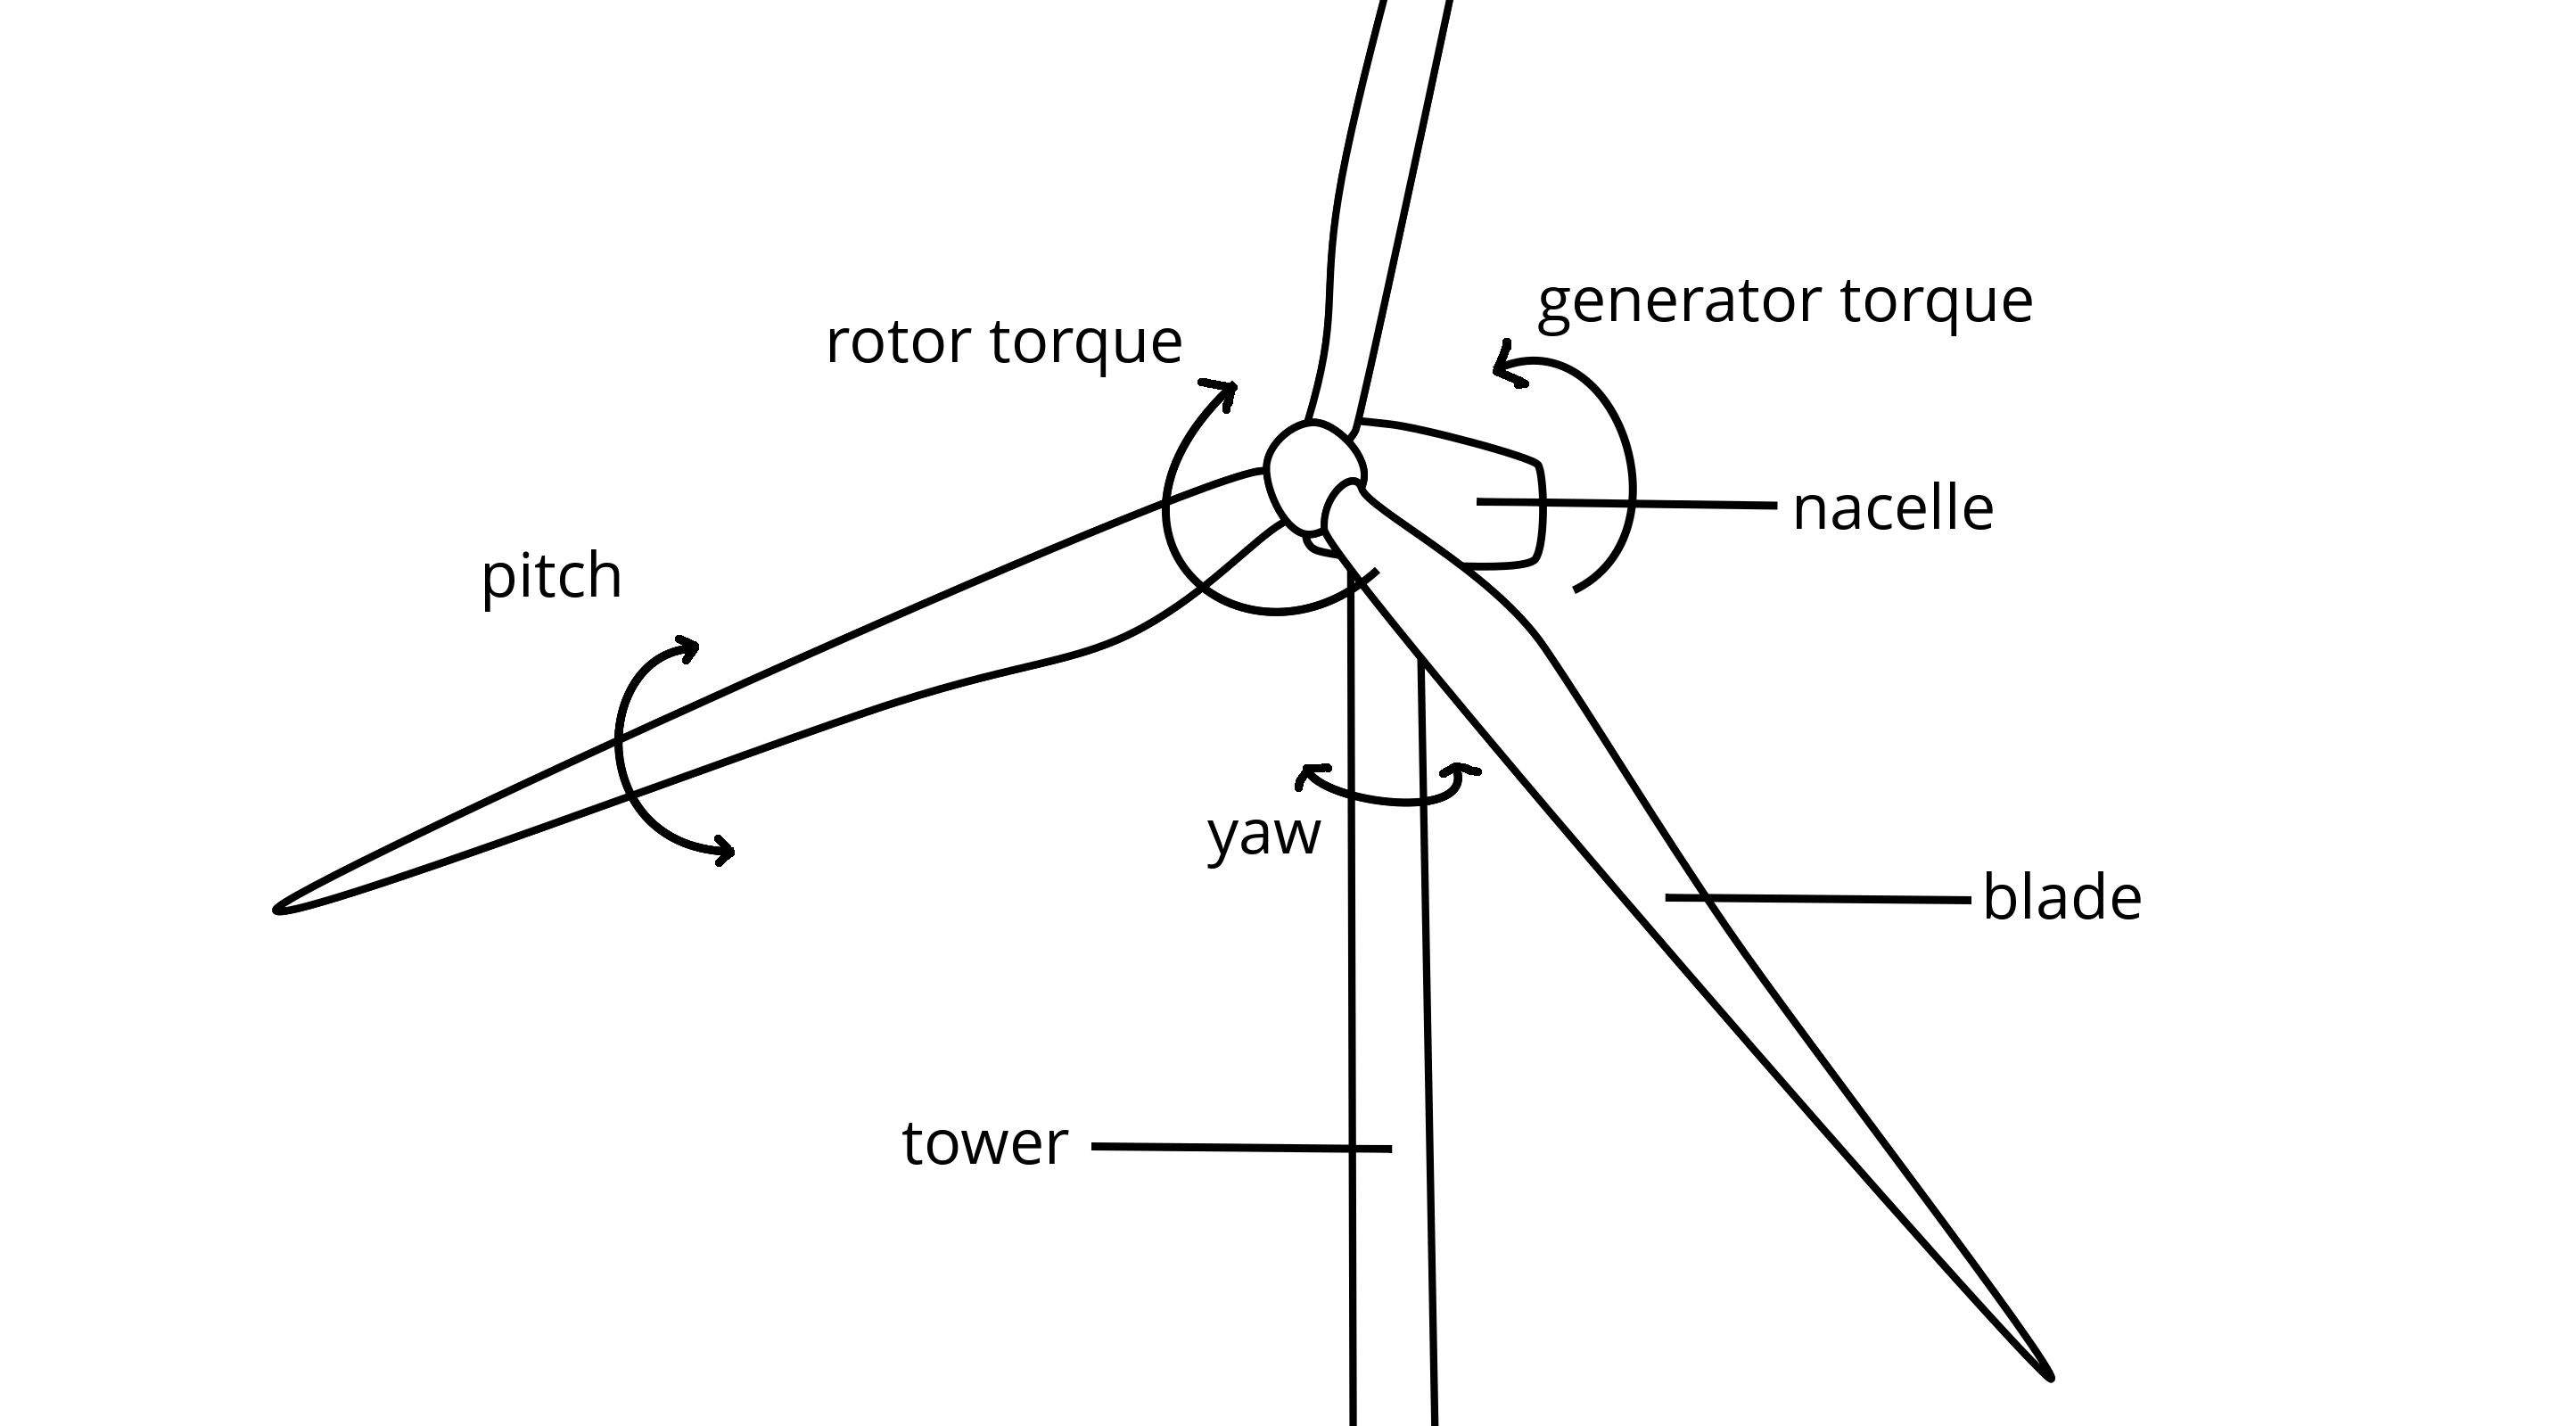
\includegraphics[width=0.7\textwidth]{images/Windturbine-Schema.png}
  \caption{A schema of the most important wind turbine components and control actions. Based on \cite{openclipartWindTurbineSketch2017}}
  \label{fig:windturbine-schema}
\end{figure}

% There are two major types of wind turbines, \acfp{VAWT} and \acfp{HAWT}. The latter proved to be suited better for large scale applications , hence we will focus this work purely on that type.
A \acf{HAWT} is the most prominent turbine design for large scale applications\cite[Chapter 1.1]{burtonWindEnergyHandbook2011}. It consists of the components shown in figure \ref{fig:windturbine-schema}. A \textit{nacelle} sits on top of a \textit{tower}. The nacelle holds a horizontal shaft with usually three \textit{blades} attached. The blades create \textit{rotor torque} through aerodynamic lift, the force that spins the rotor. The shaft is connected to a \textit{generator} inside the nacelle, which converts the rotational energy of the shaft to electric energy by applying a counteracting \textit{generator torque}. If generator torque and rotor torque match, the rotor speed stays level. The act of turning the entire nacelle on top of the tower to face the wind is called \textit{yaw} and is typically done by a yaw motor. Furthermore, the blades can be rotated along their root to tip axis to change their aerodynamic response to the incoming wind, which is called \textit{pitch}.

\begin{figure}
  \centering
  \begin{subfigure}[b]{0.32\textwidth}
      \centering
      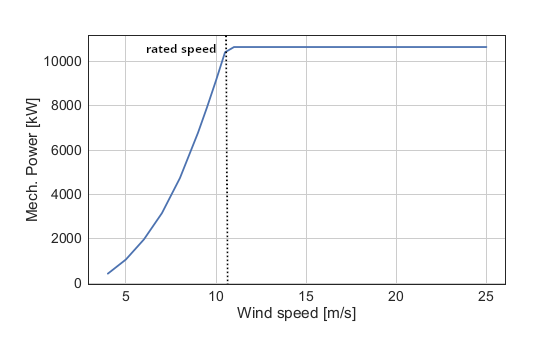
\includegraphics[width=\textwidth]{images/IEA10MW-Characteristics-1.png}
      \caption{Power production}
      \label{fig:IEA10MW-power}
  \end{subfigure}
  \begin{subfigure}[b]{0.32\textwidth}
      \centering
      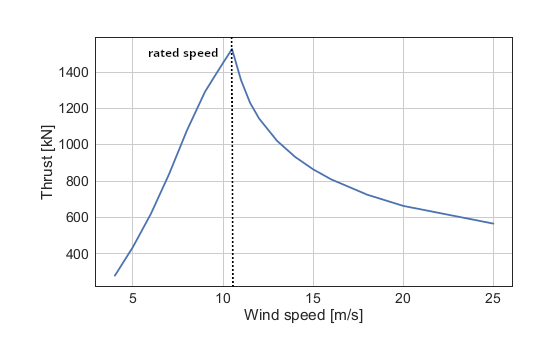
\includegraphics[width=\textwidth]{images/IEA10MW-Characteristics-2.png}
      \caption{Rotor thrust}
      \label{fig:IEA10MW-thrust}
  \end{subfigure}
  \begin{subfigure}[b]{0.32\textwidth}
    \centering
    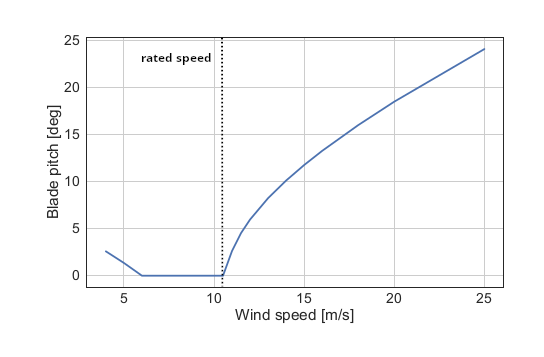
\includegraphics[width=\textwidth]{images/IEA10MW-Characteristics-3.png}
    \caption{Base pitch}
    \label{fig:IEA10MW-pitch}
  \end{subfigure}
  \caption{The steady wind operation of the 10MW IEA turbine from \citet[Figure 33]{bortolottiIEAWindTCP2019}}
  \label{fig:IEA10MW}
\end{figure}

Typically, \acp{HAWT} are designed with a specific \textit{rated wind speed} \cite[Chapter 6.3]{burtonWindEnergyHandbook2011}. This wind speed is the point above which the rotor yields more energy than the generator can convert. To prevent overheating of the generator, the aerodynamic torque produced by the rotor needs to be limited. This happens by increasing the pitch of the blades, reducing their aerodynamic efficiency. The IEA-10MW turbine has a rated wind speed of $10.75 \frac{\text{m}}{\text{s}}$ \cite[Table 16]{bortolottiIEAWindTCP2019}. In figure \ref{fig:IEA10MW} this point is visible in all three plots. Subfigure \ref{fig:IEA10MW-power} displays mechanical rotor power over wind speed, which is equal to electric turbine output, ignoring minor energy losses in the drive train, generator and inverter. From rated wind speed up, power plateaus at the rated power output, while below rated it gradually increases to maximum level. To prevent further power increase, the blade pitch angle in Subfigure \ref{fig:IEA10MW-pitch} is increased gradually from rated wind speed up, reducing aerodynamic rotor efficiency. The reduction in aerodynamic efficiency causes the thrust in Subfigure \ref{fig:IEA10MW-thrust} to decrease as well, creating a load maximum at rated speed. Similar curves are exhibited by most modern \acp{HAWT}.

A wind turbine incurs different types of loads during its life-time. Loads affect all components of the wind turbine, but for some components load reduction has a higher impact to \ac{LCOE} than for others. This can be due the high capital expenditures of building a component that can withstand high loads or due to high operating expenditures associated with maintaining them. Consulting \citet{stehly2019CostWind2020}, we identify three major components for which load reductions have a high impact on \ac{LCOE}:

\begin{itemize}
  \item The \textit{tower}, which has to carry the weight of the nacelle and rotor, absorb rotor thrust and absorb potentially occurring vibrations.
  \item The \textit{blades} are designed to be as cheap and lightweight as possible while still being able to absorb lift and gravity force. Thus, they are susceptible to load wear.
  \item \textit{Bearings and actuators} on the shaft, nacelle and blades, which are subjected to wear if they have high load moments or a lot of actuation.
\end{itemize}

Furthermore, we differentiate between \textit{fatigue loads} which are loads that occur repeatedly and accumulate over the life-time of the turbine, and \textit{extreme loads} which occur irregularly but with high amplitude, causing immediate damage. An example of fatigue loads is differing blade loads on the top and the bottom of the rotation. Extreme loads are single occurrence events, which can be induced by irregularities in the incoming wind or excessive control actions. \cite[Section 2.2]{perez-beckerAdvancedAerodynamicModeling2021}

\subsection{Optimization Aims and Wind Scenarios}
\label{section:background-optimization-aims}

\begin{summary}
This subsection describes the optimization aims relevant to this work and how they relate to different wind scenarios. For a load minimizing control policy, several conflicting optimization aims exist. Loads can be shifted from one component to another or traded for power yield. A good control policy minimizes all components wear without impacting power output. Furthermore, this section introduces the wind scenarios steady wind and turbulent wind. Steady wind is an easier scenario for control, as after one full rotation of the rotor, the turbine state is the same again, and the control policy can repeat the same actions. Turbulent wind is more challenging due to fast changes of incoming wind, but offers more optimization potential.
\end{summary}

There are several individual optimization aims for wind turbine control. Below rated wind speed, maximizing energy yield is the main aim, while other factors are secondary. Albeit load control plays a minor role below rated, the wind turbine controller seeks to have an optimal rotation speed with ideally no pitch action. This to ensure optimum energy conversion for which the turbine blades were designed for. Hence, below-rated scenarios are largely out of scope of this work. Above rated, the power is saturated, and energy yield can not increase further. Hence, load-related optimization aims become more important. At rated, a particularly challenging scenario unfolds: the power-maximizing control is switched over to a load-minimizing control when the generator becomes saturated, and at the same time, the turbine rotor experiences maximum thrust. This creates a blurry optimality criterium, as aims from below and above rated are active at the same time. Wind scenarios with changing winds that transit this operating area are difficult to optimize.

For a general load controller, \citet[Chapter 8.2.6]{burtonWindEnergyHandbook2011} list multiple optimization aims. For our work in the above-rated operating regime, we identify the following relevant quantities of interest:

\begin{itemize}
  \item Maximize energy yield
  \item Minimize fatigue loads on the blade roots
  \item Minimize extreme loads on the blade roots
  \item Minimize pitch actuation
\end{itemize}

Other performance indications like tower vibrations, nacelle and yaw bearing loads or power fluctuation are disregarded in this work to limit the scope. When applied to a real turbine, the importance of these optimization aims needs to be carefully weighted and aims disregarded in this work might become more important. Because some of these optimization aims are conflicting, trade-offs are necessary.

The easiest operating condition for a wind turbine is a steady wind scenario. In this scenario, the speed of the incoming wind is steady over time but not steady over position, meaning there can be a difference in wind speeds between two points on the rotor plane. A major contributor to those differences is a phenomenon called \textit{wind shear}, which is the difference in wind speed with height. The terrain surface slows down the wind, as obstacles are blocking the flow \cite[Table 2.1]{burtonWindEnergyHandbook2011}. Thus, wind speeds closer to the terrain surface are lower than high above the surface. The area in which this effect is observable is called \textit{planetary boundary layer}, while wind flow in the area above the boundary layer is called \textit{geostropic flow}. The wind shear effect is stronger for onshore turbine installations than offshore ones, as there are fewer obstacles to slow down the wind. Wind turbines with high output power require a large rotor, and consequently, the wind shear phenomenon is especially relevant to those high output turbines. \cite[Chapter 2.6.2]{burtonWindEnergyHandbook2011}

In the steady wind setting, extreme loads do not play a major role, as the turbine has settled to a state with constant rotor speed and constant vibrations, induced mainly by the rotor. Thus, optimizing fatigue loads is the main aim in a steady wind setting. Control strategies to reduce fatigue loads can include pitch activity to counteract wind shear and other phenomena. In the steady wind above rated speed, power yield is not subject to optimization as well, as the generator is saturated and delivers maximum energy. Only at and below rated, where the generator is not saturated, power yield must be taken into consideration.

A more challenging scenario is the turbulent wind scenario. Turbulences are caused by mainly two things, obstacles and weather effects. Obstacles such as mountains, houses or other wind turbines leave a wake with turbulent flow conditions in their down-stream area. While turbine placement takes these factors into consideration, it is impossible to rule out obstacle induced turbulence. Thermal convection effects in the atmosphere, which range from local temperature-difference induced perturbations to larger weather scenarios like thunderstorms have the potential of inducing heavy turbulences \cite[Chapter 2.6.1]{burtonWindEnergyHandbook2011}. These effects induce swirls (\textit{eddies}) in the airflow. Rapid and unpredictable changes of wind direction and speed across the rotor plane are the result. Turbulent eddies occur in all scales including sub-rotor scales, often presenting different inflow conditions to the different blades. 

Modelling turbulence is not trivial, and there are various common stochastic estimations for turbulence. Examples for these are the Kaimal and the von Karman spectra \cite[Section 2.6.4]{burtonWindEnergyHandbook2011}. The IEC 61400-1 standard \cite{internationalelectrotechnicalcommissionIEC61400120192019} defines parametrizations of these spectra through which a turbulent wind field can be artificially modelled:

\begin{itemize}
  \item \acf{NTM}
  \item \acf{ETM}
  \item \acf{EWM}
\end{itemize}

When designing a wind turbine, it has to pass tests in all these turbulence models and many more design load cases. Hence, a controller needs to be able to cope with these turbulence models. Specifically, it shall minimize fatigue loads and keep extreme loads below a threshold set by the structural design of the turbine despite the challenging and unpredictable inflow.

In the turbulent wind setting, a complex trade-off between fatigue loads and extreme loads of different components and power yield is subject to optimization. Especially around rated speed, rotor thrust can dip below generator saturation level, consequently maximizing power production is a concern in this wind setting. Pitch actuator wear should be kept at a minimum by minimizing pitch activity. At the same time, blade fatigue loads shall be minimized by reducing vibrations, which can be done by using a corrective pitching action or lowering the power level. Finally, blade extreme loads should be minimized by using preventive pitching actions, which goes at the expense of pitch wear and power production. If a policy succeeds in improving all quantities of interest, it is strictly better than a previous policy. But also, finding a trade-off between pitch fatigue loads, blade fatigue loads, blade extreme loads, and power production that adheres optimally to the requirement of the turbine is desirable.



\subsection{Sensor Overview}

\begin{summary}
This section presents the data available to the reinforcement learning algorithm. The sensor configuration varies between turbine models, and in this work, we select our data from commonly installed sensors.
\end{summary}

There are different types of sensors measuring the operating state of the wind turbine. While some sensors are installed in all turbines, others are only found in modern or research turbines. This section gives an overview of the types of sensors relevant to this work and whether they can be assumed installed or not.

\begin{enumerate}
  \item \textbf{Rotational speed} ($\srot$) Measures the angular velocity or rotational speed of the rotor. This sensor is present on all regulated wind turbines, as it is the fundamental input for both torque and pitch controllers. Usually, there are several rotational speed sensors to increase fault-tolerance.
  \item \textbf{Azimuth angle} ($\sazi$) Measures the point of the rotation the rotor is at. The azimuth can be inferred from the rotational speed or vice versa. This can be assumed present on all regulated wind turbines.
  \item \textbf{Generator power} ($\spow$) Generator output power is a fundamental metric, which is necessary for the wind park operator, and thus is measured on all wind turbines.
  \item \textbf{Pitch angle} ($\spitchx$) If a turbine has one or more pitch actuators, the actuation position needs to be known for the pitch actuation controller. This work only deals with pitch actuated turbines on which this signal can be assumed present.
  \item \textbf{Out-of-plane blade root bending moments (\textit{\acs{BRBM}})} ($\soopbend$) In this work also referred to as \textit{blade bendings}, are measured on all wind turbines which implement the \ac{IPC} strategy. Older or smaller turbines operating under a \ac{CPC} strategy usually lack this signal. The \ac{BRBM} are obtained through the measurement of strain gauges installed at specific positions of the blade root. Through the proper calibration, the strain information can be converted to bending moment data. 
  \item \textbf{Tower bending moments} ($\stbend$) Measures the load on the tower. This can either be obtained through force sensors embedded into the tower or through accelerometers in the nacelle. Accelerometers are used by the supervisory controller and to regulate tower vibrations, and are installed on most modern turbines, even smaller ones.
\end{enumerate}

There are further sensors, which can be installed on some modern and research turbines. Examples for these are in-plane or torsional blade root bendings, yaw bearing moments, blade-wise inflow sensors \cite{jonesOvercomingFundamentalLimitations2018}, LIDAR-sensors \cite{bossanyiWindTurbineControl2014} and others. Presence of these sensors is not necessary for the approach presented in this work.

\subsection{Wind Turbine Control Types}

\begin{summary}
This subsection discusses the different control subsystems which make up a wind turbine controller. Our work is limited to closed-loop control and disregards supervisory and safety tasks such as startup, shutdown or handling of emergency situations.
\end{summary}

A wind turbine controller has the task of adjusting the output signals such as actuators optimally while adhering to the operational and structural limits of the turbine. Optimality in the case of wind turbines involves trade-offs, as the individual optimization aims are partially conflicting. The current operating state is usually determined from a number of input signals such as sensors and the controller state. To achieve safe and efficient control, typical wind turbine control systems are divided into several subsystems: \cite[Chapter 8.1]{burtonWindEnergyHandbook2011}

\begin{itemize}
  \item A \textit{supervisory controller} which has the task of managing the high-level state of the turbine during normal operation. Typical states could include startup, shutdown and power production. The supervisory controller provides software fail-safes that automatically transition to shutdown in case of any abnormalities.
  \item A \textit{closed-loop controller} which is only active in the power production state. This controller sets the turbine controls to yield the maximum amount of energy possible while keeping loads at a minimum.
  \item A \textit{safety system} which is normally implemented in hardware. It has the task of bringing the turbine to a halt in case of an emergency when the supervisory controller appears to be unable to do so and should work in the presence of severe failure conditions.
\end{itemize}

In this work, we focus on the closed-loop controller only and refer to this subsystem by \textit{controller}.

\subsection{Yaw-, Pitch- and Torque Controllers}
\label{section:background-closed-loop}

\begin{summary}
In the following subsection we will give a brief overview of the closed-loop control systems with an emphasis on the pitch controller. Pitch control has the job to regulate the aerodynamic thrust of the rotor and can be used to additionally perform load control. Our work aims at improving upon current state-of-the-art pitch control policies.
\end{summary}

There are three major closed-loop control systems on modern wind turbines: \textit{yaw-, pitch and torque control}. The nacelle can be rotated on the tower, creating a yaw motion to face the find. Either all blades collectively (\textit{collective pitch}) or each blade individually (\textit{individual pitch}) can be turned in bearings at the blade root connection, creating a pitching motion. In some turbines, especially in turbines that are not limited to a single rotor speed for operation, the generator torque is controlled through an additional closed-loop system.

\subsubsection{Yaw Control}
Most wind turbines are stable in yaw, meaning the aerodynamic nature of the rotor causes it to automatically rotate into the wind without additional control needed \cite[Chapter 3.10]{burtonWindEnergyHandbook2011}. However, some active yaw control is usually in place. For this, a heavily averaged signal from the wind vein on top of the nacelle is the criterium to start a slow-moving yaw motion if the deviation is greater than a specified value \cite[Chapter 8.2.4]{burtonWindEnergyHandbook2011}. Recently, yaw control has found new applications when optimizing control policies for an entire wind farm through \textit{wake steering} \cite{howlandWindFarmPower2019}.

As for a single turbine, yaw control is relatively trivial, we will exclude yaw control in this work and assume a default yaw control strategy in place.

\subsubsection{Torque Control}
Wind turbines with a fixed rotor speed do not allow generator torque control. The IEA-10MW turbine however implements torque control, as it tolerates rotor speeds in the region of 6 to 8.68 rpm \cite[Table 16]{bortolottiIEAWindTCP2019}. Above rated wind, a common strategy for torque control is to set the torque to maximum and allow the pitch controller to adjust the rotor speed. Below rated, the rotor speed can be adjusted to an aerodynamically optimal setting for the wind speed by changing generator torque. \cite[Chapter 8.2.3]{burtonWindEnergyHandbook2011}

As we are concerned with fatigue and extreme loads, which mainly occur around and above rated speed, torque control plays a minor role in this work.

\subsubsection{Pitch Control}

The pitch control system is mainly used for power regulation and in some turbines load control above rated wind. Below rated wind, it helps the torque controller with power maximization. There is an aerodynamically optimal pitch angle at which the rotor generates the maximal torque for most wind speeds. Below rated, the task of the pitch controller is to match this pitch setting. On many turbines including the IEA-10MW turbine, this optimal pitch angle is zero degrees with minor adjustments in very low winds. Above rated, the pitch controller reduces the aerodynamic efficiency to prevent overloading the generator. Depending on the airfoils used, pitch can be either increased or decreased away from the optimal angle to reduce the aerodynamic efficiency of the blades. The prevalent mode in most turbines is to increase pitch, which is called pitching towards \textit{feather}. The IEA-10MW turbine \cite[Table 17]{bortolottiIEAWindTCP2019} in this work pitches towards feather and has an optimal angle of zero degrees, i.e. increasing the pitch reduces the aerodynamic efficiency of the rotor. Next to regulating turbine power, the pitch controller also has the task of performing load control. With correct timing of pitch signals, the blade loads can be distributed evenly across the three blades and across time to minimize wear. Harmonic frequencies of structural elements can be counteracted by a suitable pitch motion, and extreme loads from turbulences can be mitigated. This load reduction task is the main focus of the work. \cite[Chapter 8.2.1]{burtonWindEnergyHandbook2011}

There are two major classes of pitch controllers, \textit{collective} pitch controllers and \textit{individual} pitch controllers. In collective pitch, all three blades are always set to the same pitch angle, while in individual pitch, the individual blades are controlled separately with different pitch actions. It is a common procedure in the design of individual pitch controllers to use the collective pitch signal from a collective controller as a signal to build individual pitch policies upon. This way, separation of concerns is introduced where the collective pitch controller has the main task of regulating rotor torque while the individual pitch controller can focus on load control.

\subsection{Collective Pitch Control}
\label{section:background-cpc}

\begin{summary}
This subsection introduces the less complicated of our two evaluation benchmarks, the \acf{CPC}. We describe a CPC formulated as a PID controller.
\end{summary}

Collective pitch control is normally based on a single \acf{PID} with the formula as in Equation \ref{eq:pitch_pid}:

\begin{equation}
  \apitch(t) = \pidgainp e(t) + \pidgaini \sum_{T=0}^t e(T)  + \pidgaind \frac{\Delta e(t)}{\Delta t}
\label{eq:pitch_pid}
\end{equation}

with $e(t) = \hat \srot(t) - \srot(t)$ being the error term at timestep $t$ between measured rotor speed $\srot$ and desired rotor speed $\hat \srot$. The parameters $\pidgainp$, $\pidgaini$ and $\pidgaind$ are derived using a variety of methods from control theory, usually involving a linearized model of the turbine and a closed-form solution to the optimal parameters under certain working conditions. If $\pidgaind$ is zero, the controller is called a \textit{PI controller}. Additional techniques to improve the performance of this construct include:

\begin{itemize}
  \item Introducing bandpass, lowpass, highpass, or notch filters to lower or raise responses in certain frequency regions. By matching the filters to avoid harmonic frequencies of the tower or blades, vibration is reduced \cite{bossanyiFurtherLoadReductions2005}.
  \item \textit{Integrator desaturation}, a technique to counteract the integrator component accumulating error in below-rated regions where the desired rotor speed is lower than the target rotor speed for the pitch controller \cite[Chapter 8.2.7]{burtonWindEnergyHandbook2011}.
  \item \textit{Gain scheduling}, a technique where different PID constants are used depending on the operating scenario of the wind turbine \cite[Chapter 8.4]{burtonWindEnergyHandbook2011}.
\end{itemize}

In our work, we use the CPC from \citet{perez-beckerImplementationValidationAdvanced2021} with these features as an evaluation benchmark to compare to our control strategy. The CPC policy is optimal with respect to pitch wear, meaning there is no control policy that induces less pitch wear while maintaining power regulation.

\subsection{Individual Pitch Control For Load Reduction}
\label{section:background-ipc}

\begin{summary}
This section presents the second evaluation benchmark, the \acf{IPC} \cite{bossanyiIndividualBladePitch2003}. This control policy is more complex than a \ac{CPC} and has been recently implemented in some large wind turbines. It builds upon the Coleman Transformation \cite{birMultibladeCoordinateTransformation2008}, which we use for pre- and postprocessing in the reinforcement learning pipeline. This transformation converts between the rotating coordinate system of the rotor into a stationary coordinate system along the rotor plane, and as such, simplifies information processing.
\end{summary}

A major factor for blade fatigue loading is the difference in wind speed at different parts of the rotor. Specifically, \textit{wind shear}, the increase in wind speed with height, can be the cause of major load differences during a rotation of the rotor. \cite[Chapter 2.6.2]{burtonWindEnergyHandbook2011} To counteract this phenomenon, \citet{bossanyiIndividualBladePitch2003} \cite{bossanyiFurtherLoadReductions2005} have developed a control strategy which exploits the ability of some modern wind turbines to actuate each blade pitch individually.

To achieve \acf{IPC}, \citet{bossanyiIndividualBladePitch2003} work in a transformed coordinate system, which they call the \textquote{d-q Axis Transformation}. This transformation is a special case of the \textit{Coleman Transformation}, which will be presented later in this section. The forward transformation is described in Equation \ref{eq:dq-axis-transform}:

\begin{equation}
\begin{pmatrix}
  c_d \\ c_q
\end{pmatrix}
=
\frac{2}{3}
\begin{pmatrix}
  \cos(\sazi) & \cos(\sazi + \frac{2 \cpi}{3}) & \cos(\sazi + \frac{4 \cpi}{3}) \\
  \sin(\sazi) & \sin(\sazi + \frac{2 \cpi}{3}) & \sin(\sazi + \frac{4 \cpi}{3})
\end{pmatrix}
\begin{pmatrix}
  \soopbenda \\
  \soopbendb \\
  \soopbendc
\end{pmatrix}
\label{eq:dq-axis-transform}
\end{equation}

where $\cpi$ references the circle constant commonly denoted as $\pi$, $\sazi$ is the rotor azimuth angle in radians, and $[\soopbenda, \soopbendb, \soopbendc]$ the \ac{BRBM} of blade 1-3. The resulting variables $c_d$ and $c_q$ are the equivalent tilting and yawing moments of the rotor. The arise because of a difference effective force distribution on the rotor. $c_d$ is positive if there is more force and hence more bending in the upper half of the rotation than in the lower. $c_q$ is positive if there is more force in the right half of the rotation than in the left.

The reverse transformation is described in Equation \ref{eq:dq-axis-backtransform}:

\begin{equation}
  \begin{pmatrix}
    \apitchad \\
    \apitchbd \\
    \apitchcd
  \end{pmatrix}
  =
  \begin{pmatrix}
    \cos(\sazi) & \sin(\sazi) \\
    \cos(\sazi + \frac{2\cpi}{3}) & \sin(\sazi + \frac{2\cpi}{3}) \\
    \cos(\sazi + \frac{4\cpi}{3}) & \sin(\sazi + \frac{4\cpi}{3})
  \end{pmatrix}
  \begin{pmatrix}
    c_D \\ c_Q
  \end{pmatrix}
\label{eq:dq-axis-backtransform}
\end{equation}
where $\cpi$ references the circle constant, $\sazi$ is the rotor azimuth angle in radians. $[\apitchad, \apitchbd, \apitchcd]$ are the differences to the collective pitch signal with the actual pitch signal, which can be recovered like $\apitcha = \apitch + \apitchad$. $c_D$ and $c_Q$ are control signals representing the required pitch actuation in the non-rotating coordinate system to compensate for the yawing and tilting moments on the rotor. If $c_D$ is positive, there is positive pitch offset in the upper half of the rotation and negative pitch offset in the lower. If $c_Q$ is positive, there is positive pitch offset in the right half of the rotation and negative in the left.

Finding $c_D$ and $c_Q$ is the task of the control policy. For this, an LGQ algorithm \cite{bossanyiIndividualBladePitch2003} or a PID based algorithm \cite{bossanyiFurtherLoadReductions2005} can be used.

\begin{figure}
  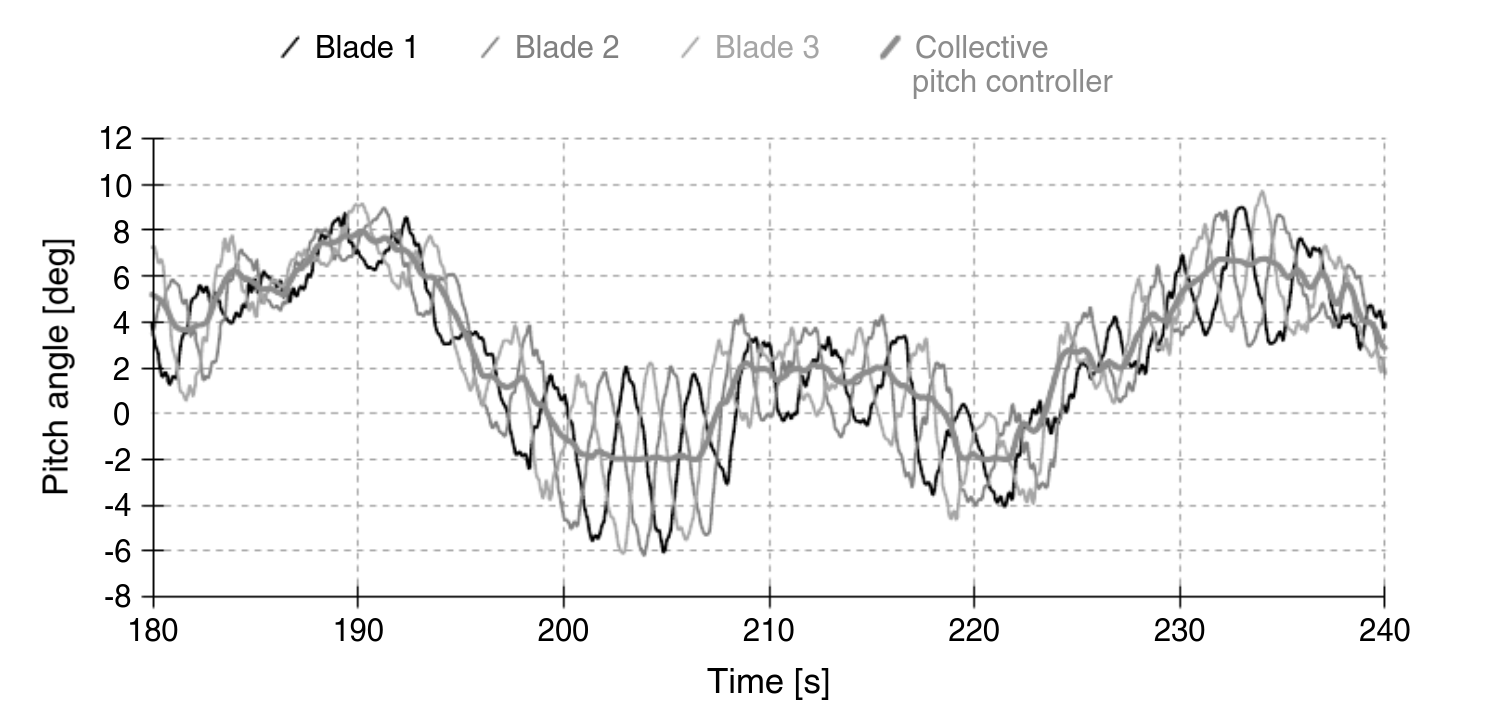
\includegraphics[width=\textwidth]{images/IPC-reference.png}
  \caption{An example pitch plot taken from \citet[Figure 2]{bossanyiIndividualBladePitch2003} for an IPC controller for a 5MW turbine in a turbulent wind scenario.}
  \label{fig:ipc-reference}
\end{figure}

As visible in Figure \ref{fig:ipc-reference}, this strategy results in a three-phase sinusoidal actuation of the three blades, with the center of the sine being the collective pitch action. In the plot, both the collective pitch action and the IPC amplitude change over time due to changes in the incoming wind. A higher pitch angle corresponds to a higher incoming wind speed. If a high difference between top and bottom loads is encountered, the resulting sine has a high amplitude, while low load differences create a low amplitude sine. In the steady wind, most of the load differences are caused by wind shear. Hence, positive deviations from collective pitch happen mostly in the upper half of the rotation, while the negative deviation happens in the lower half of the rotation. In the turbulent wind, large turbulence eddies or spontaneous inflow angle changes can have both tilting and yawing effects resulting in a more chaotic pitching pattern. The center of the sines, the baseline collective pitch actuation, is determined as usual, e.g. through a \ac{PID} controller to regulate rotor speed.

The d-q Axis Transformation is closely related to the \textit{Coleman Transformation} \cite{birMultibladeCoordinateTransformation2008}. The Coleman Transformation can be thought of as an extension to the $c_d$-$c_q$ Axis Transformation by an additional parameter $c_s$ which marks a constant offset independent of the azimuth angle. The forward transform of a first order Coleman Transformation works as described in Equation \ref{eq:coleman-forward} and the backward transform as in \ref{eq:coleman-backward}. 

\begin{equation}
  \begin{pmatrix}
    c_s \\ c_d \\ c_q
  \end{pmatrix}
  =
  \begin{pmatrix}
    \frac{1}{3} & \frac{1}{3} & \frac{1}{3} \\
    \frac{2}{3} \cos(\sazi) & \frac{2}{3} \cos(\sazi + \frac{2\cpi}{3}) & \frac{2}{3} \cos(\sazi + \frac{4\cpi}{3}) \\
    \frac{2}{3} \sin(\sazi) & \frac{2}{3} \sin(\sazi + \frac{2\cpi}{3}) & \frac{2}{3} \sin(\sazi + \frac{4\cpi}{3})
  \end{pmatrix}
  \begin{pmatrix}
    \soopbenda \\
    \soopbendb \\
    \soopbendc
  \end{pmatrix}
  \label{eq:coleman-forward}
\end{equation}

\begin{equation}
  \begin{pmatrix}
    \apitchad \\
    \apitchbd \\
    \apitchcd
  \end{pmatrix}
  =
  \begin{pmatrix}
    1 & \cos(\sazi + \philead) & \sin(\sazi + \philead) \\
    1 & \cos(\sazi + \philead + \frac{2\cpi}{3}) & \sin(\sazi + \philead + \frac{2\cpi}{3}) \\
    1 & \cos(\sazi + \philead + \frac{4\cpi}{3}) & \sin(\sazi + \philead + \frac{4\cpi}{3})
  \end{pmatrix}
  \begin{pmatrix}
    c_S \\ c_D \\ c_Q
  \end{pmatrix}
\label{eq:coleman-backward}
\end{equation}

The backward transformation offers an azimuth offset angle $\philead$, which can be used to modify the coordinate system of the backtransform slightly. Slow acting pitch actuators can this way receive their signal a little before they reach the point of the rotation where the signal should be applied. The extended Coleman transformation offers extra freedom over the $c_d$-$c_q$ transformation, which can yield better control strategies. For an example design process, see \citet{luAnalysisDesignColeman2015}.

\subsection{Damage Equivalent Loads}
\label{section:damage-equivalent-loads}

\begin{summary}
This subsection presents an evaluation metric widely used in wind turbine research, the \acf{DEL}. Lower \acsp{DEL} are closely related to reduced long-term component wear, which is an important aim of load minimization. DELs can be computed for different components, taking into account their respective material properties.
\end{summary}

As a meaningful metric for load comparison, \acfp{DEL} has become a defacto standard in wind turbine control. \acp{DEL} are calculated using the \textit{rainflow counting} algorithm \cite{matsuichiFatigueMetalsSubjected1968} combined with the Palgrem-Miner rule \cite{minerCumulativeDamageFatigue1945}. The algorithm takes as input a time series and outputs a bending moment value that creates the same damage when applied for the same duration to the same material at a given frequency as the time series. More intuitively, when a component like a blade experiences some really high loads and a lot of smaller loads across a time series, the resulting DEL would lay somewhere in between, as a repeated loading in between would induce the same amount of damage to the blade. There are a series of assumptions for DELs to be accurate and some corrections to make up for violated assumptions, such as the Goodman correction \cite[Equation 29]{haymanMLifeTheoryManual2012}. In this work, the uncorrected \ac{DEL} calculation is used, as they form a standard in academia and industry to quickly and easily compare control strategies.

To compute the metric, load cycles over a signal are extracted through \textit{Rainflow-Counting} \cite{matsuichiFatigueMetalsSubjected1968}. A load cycle in this sense is the bending of a component one way (half cycle) or back and forth (full cycle). Rainflow-Counting returns, among other metrics, load cycle ranges $\rainflowrange$ and counts $\rainflowcount$ for all load cycles $i$ in the signal $x$. Furthermore, most Rainflow implementations offer a binning, where ranges close to each other are binned to the same range with a higher count. The Formula for calculating the damage equivalent load given the rainflow counting results after \citet[Equation 26, 30]{haymanMLifeTheoryManual2012} is described in Equation \ref{eq:del}:

\begin{equation}
  \del(x, \woehler, \fdel) = \left( \frac{\sum_i{(\rainflowcount (\rainflowrange)^\woehler})}{\fdel T_x} \right)^{\frac{1}{\woehler}}
  \label{eq:del}
\end{equation}

with $\woehler$ being the Wöhler exponent, which is specific to the component materials subjected to the loads, $T_x$ being the total simulation time of the signal in seconds, and $\fdel $ being the DEL frequency. This frequency is the aforementioned frequency, to which all loads in the signal shall be mapped. The Wöhler exponent is a single number, which approximates a \textit{SN-curve}. This curve characterizes the number of load cycles (\textit{N}) for a stress force (\textit{S}) required for the component to break. Knowledge of an SN-curve for a material type or component makes it possible to predict the time to failure under known fatigue loads. Through the Wöhler exponent, the SN-curve of a component is modeled into the DEL calculation, where a higher exponent means a lower sensitivity to low-magnitude stresses and a higher sensitivity to extreme-load stresses. \cite{blasquesMeanLoadEffects2013} \cite{freeburyDeterminingEquivalentDamage2000}



\chapter{Approach}
\label{ch:approach}

This chapter presents the contribution of this work, first in a generalized form and later with details specific to our implementation.

\section{WINDL - A Novel Approach To Wind Turbine Control With RL}
\label{section:approach-theory}

\begin{summary}
We present \acf{WINDL}. This section introduces an abstract view of our framework. Main design choices were made regarding the reinforcement learning algorithm, the pre- and post-processing pipeline, and reward shaping. Furthermore, we outline our training process and evaluation methods.
\end{summary}

The fundamental interaction cycle of reinforcement learning (see Figure \ref{fig:rlcycle}) assumes a direct link between the environment and the agent. While it would be mathematically possible to directly feed simulation outputs into the reinforcement learning algorithm and vice versa, we found this to be infeasible in practice. Hence, we introduce a pre- and postprocessing architecture to facilitate learning.

The high-level architecture is described in Figure \ref{fig:high-level-schema}. A wind turbine \textit{simulation} (see Section \ref{section:approach-simulation}) outputs sensor data for every time step, which is fed into a \textit{preprocessing pipeline} (see Section \ref{section:approach-preprocessing}). The output of this pipeline is a state vector and a reward signal (see Section \ref{section:approach-reward-shaping}) which is used as a neural network input in the \textit{agent}. The agent is trained within the \textit{RL algorithm} (see Section \ref{section:approach-rl-algorithm}) to optimize reward. The agent output actions in the Coleman transformed space which are processed to pitch angles in the \textit{postprocessing pipeline} (see Section \ref{section:approach-postprocessing}). These pitch angles are used, together with assistive control actions, as a simulation input (see Section \ref{section:approach-simulation}). From there, the cycle restarts.

\begin{figure}
  \centering
    \begin{tikzpicture}
      \node (sim) [process] {Simulation};
      \node (pre) [process, above right = 0.5cm and 2.5cm of sim] {Preprocess};
      \node (agent) [process, below right = 0.5cm and 2.5cm of pre] {Agent};
      \node (post) [process, below right = 0.5cm and 2.5cm of sim] {Postprocess};

      % \draw [arrow,out=90,in=180] (sim.north) to node[left]{action $a$} (pre.west);
      \draw [arrow] (sim.north) |- node[pos=0.7,above] {$\spitchx_{1-3}, \soopbend_{1-3}, \srot, \spow, \sazi, \stbend_{x,y}$} (pre.west);
      \draw [arrow] (pre.east) -| node[pos=0.25,above] {$s,r$} (agent.north);
      \draw [arrow] (agent.south) |- node[pos=0.75,above] {$a$} (post.east);     
      \draw [arrow] (post.west) -| node[pos=0.25,above] {$\apitchx_{1-3}$} (sim.south);
  
    \end{tikzpicture}
  
    \caption{High-Level schema of \ac{WINDL}}
    \label{fig:high-level-schema}
\end{figure}

\subsection{Preprocessing Simulation States}
\label{section:approach-preprocessing}

\begin{summary}
This subsection describes the preprocessing procedure, which most notably transforms the raw sensor data into a stationary coordinate system through the Coleman transformation and normalizes it.
\end{summary}

Final policy performance is greatly influenced by the quality of pre- and postprocessing of the data. A couple of techniques are common to the entire field of machine learning, like normalization, removal of low quality or unnecessary data and transformations into a format more easily processable for neural networks. Each neural network architecture has slightly different requirements concerning the normalization range, input format, and sensitivity to inaccurate data. Reinforcement learning is no exception to this. However, in contrast to supervised or unsupervised machine learning, pre- and postprocessing can not happen beforehand but has to happen in the sampling loop. We preprocess simulation outputs through the selection of inputs, normalization, a modified Coleman transformation, a Cartesian transformation, and dilated past feeding. 

Wind turbine simulations naturally offer a high number of measurement signals, however on a real wind turbine, the number of sensors is limited due to cost and complexity considerations. For our algorithm, we chose to include the following inputs, which are already measured on most modern turbines:
\begin{itemize}
  \item Rotor speed $\srot$
  \item Generator power $\spow$
  \item Pitch angles $\spitchx_{1-3}$
  \item Out of plane blade root bending moments $\soopbend_{1-3}$
  \item Tower bottom bending moment in wind direction $\stbendx$  
  \item Tower bottom bending moment orthogonal to wind direction $\stbendy$
  \item Azimuthal position of the rotor $\sazi$
\end{itemize}

These values are used as an input to the preprocessing pipeline. Note that we do not utilize wind speed as a signal, as obtaining this is notoriously hard. Anemometers on top of the wind turbine are in the wake effect of the rotor and thus do not give sensible measurements. Furthermore, measuring a single point on the rotor plane with an anemometer does not give much insight into the state at other points on the rotor plane, especially in turbulent winds with strongly local turbulence effects. Through the use of neural networks, including more sophisticated sensor arrays such as LIDARs or local blade inflow measurements is possible, but remains open to future work. 

\begin{figure}
  \centering
  \begin{tikzpicture}
    \node (cartesian) [process] {Cartesian Transform};
    \node (coleman) [process, below = 2cm of cartesian] {Coleman Transform};
    \node (normalization) [process, below right = 0.5 and 0.5cm of cartesian] {Normalization};
    \node (past) [process, right = 1.5cm of normalization] {Dilated Past Feeding};
    \node (reward) [process, below = 2cm of normalization] {Reward};

    \coordinate [left = 1.5cm of cartesian.west] (cartesianin);
    \coordinate [left = 1.5cm of coleman.west] (colemanin);
    \coordinate [left = 5.25cm of normalization.west] (normalizationin);
    \coordinate [left = 5.25cm of reward.west] (rewardin);
    \coordinate [right = 1cm of past.east] (pastout);
    \coordinate [right = 5.75cm of reward.east] (rewardout);

    \draw [arrow] (cartesianin) to node[above]{$\sazi$} (cartesian.west);
    \draw [arrow] (colemanin) to node[above]{$\soopbend_{1-3}$}(coleman.west);
    \draw [arrow] (normalizationin) to node[above]{$\spitchx_{1-3}, \soopbend_{1-3}, \srot, \spow, \stbend_{x,y}$}(normalization.west);
    \draw [arrow] (rewardin) to node[above]{$\spitchx_{1-3}$} (reward.west);
    \draw [arrow] (past.east) to node[above]{$s$} (pastout);
    \draw [arrow] (cartesian.east) -| node[pos=0.25,above]{$\cartazix, \cartaziy$} (normalization.north);
    \draw [arrow] (coleman.east) -| node[pos=0.25, above]{$\tilde{c_s}, c_d, c_q$} (normalization.south);
    \draw [arrow] (coleman.east) -| (reward.north);
    \draw [arrow] (normalization.east) to node[above]{$s_{comp}$} (past.west);
    \draw [arrow] (reward.east) to node[above]{$r$} (rewardout);

  \end{tikzpicture}

  \caption{Preprocessing pipeline}
  \label{fig:preprocessing-pipeline}
\end{figure}

Figure \ref{fig:preprocessing-pipeline} shows the components of the preprocessing pipeline. Bending moments $\soopbend_{1-3}$ and azimuth angle $\sazi$ are transformed to a more suitable coordinate system and added back to the state vector. Then, the entire state vector is fed through a normalization component to make the input suited for gradient computation through backpropagation. The normalized outputs are then enriched with information from past steps to ensure the Markov property before they are fed to the neural network. The reward function utilizes information from the transformed bending moments and the pitch angles and is a heuristic for blade and pitch wear.

More precisely, we employ a Coleman Transformation for the bending moments as noted in Equation \ref{eq:coleman-forward}. $c_d$ and $c_q$ are concatenated to the state space, while $c_s$ is highpass-filtered to $\tilde{c_s}$ before concatenation. Furthermore, the untransformed bending moments are part of the state space as well, as this redundant inclusion of transformed and untransformed moments improved performance empirically. We transform the rotor azimuth to Cartesian coordinates on a unit circle and concatenate $\cartazix$ and $\cartaziy$ to the state space. Here, using the untransformed azimuth angle did not play out favorably, so it is dropped from the state vector. As simulation outputs are several orders of magnitude away from each other, we employ a running normalization which we seed with pre-computed values from past runs. We normalize to mean 0 and standard deviation 1 on all input signals. As the state space does not fulfill the Markov property, we employ the trick from \citet{mnihPlayingAtariDeep2013} of concatenating past states to the current one. Improving upon this, we employ a technique which we call \textit{dilated past feeding}. The 15-element state vector $s_{comp}$, which is output by the normalization process, is shown in Equation \ref{eq:state-vector}:

\begin{equation}
  s_{comp} = \text{norm} \left(
  \begin{bmatrix}
    \srot &
    \spow &
    \spitcha &
    \spitchb &
    \spitchc \\
    \soopbenda &
    \soopbendb &
    \soopbendc &
    \stbendx &
    \stbendy \\
    \tilde c_s &
    c_d &
    c_q &
    \cartazix &
    \cartaziy
  \end{bmatrix} 
  \right) \in \mathbb{R}^{15}
  \label{eq:state-vector}
\end{equation}

with $\srot$ being the current rotational speed, $\spow$ the current output power, $[\spitcha, \spitchb, \spitchc]$ the measured pitch angles from the simulation, $[\soopbenda, \soopbendb, \soopbendc]$ the out-of-plane bending moments, $[\stbendx, \stbendy]$ the tower bottom bending moments along and orthogonal to the wind direction, $[\tilde{c_s}, c_d, c_q]$ being the output of the modified Coleman transformation and $[\cartazix, \cartaziy]$ being the azimuth angle $\sazi$ in a Cartesian coordinate system. The final state vector $s$ after dilated past feeding has a dimension multiple of 15, as past feeding concatenates copies of this vector from different points in the past together.

\subsubsection{Cartesian Transformation}

The raw azimuth angles from the simulation form a sawtooth pattern, which linearly rises from 0 to 360 degrees and then drops back to zero in one timestep. This means there is a large difference between the azimuth input for 359 and 1 degree, albeit the actual difference in rotor position is minimal. To give a smoother input, we transform the azimuth to cartesian coordinates on a unit circle with $\cartazix = \sin(\sazi)$, $\cartaziy = \cos(\sazi)$ and drop the raw azimuth angle.

\subsubsection{Normalization}

Using a normalization improves backpropagation performance. Mathematically it is not necessary as the first-layer weights could perform any normalization and the gradient calculation process is mathematically independent of the range of input values. However, experience has shown that the backpropagation algorithm performs better with normalized values as gradient errors are dependent on the magnitude of input values and could cancel out effective gradient updates. 

For some architectures like ResNets, there is a fixed normalization target, to which inputs should be normalized to. To our knowledge, no strict normalization targets are established for the fully connected network in use in our work. Hence, we choose to normalize to mean 0 and standard deviation 1.

We use a running normalization to continuously update our normalization parameters to match the stream of observations that is being fed in through the pipeline. The longer the training runs, the smaller the step size with which we update our normalization to avoid interfering with the learning process. To avoid strong updates at the beginning, we seed our normalization with precomputed parameters.

Welford's algorithm \cite{welfordNoteMethodCalculating1962} for estimating both means and variances in one pass is numerically stable and can calculate a running normalization. The running mean is computed intuitively like Equation \ref{eq:welford-mean}:

\begin{equation}
  \bar{x}_n = \bar{x}_{n-1} + \frac{x_n - \bar{x}_{n-1}}{n}
  \label{eq:welford-mean}
\end{equation}

with $x_n$ being the original signal at sampling point $n$, and $\bar{x}_n$ the estimation of the running mean at sampling point $n$. The running variance estimation works by keeping a sum of squared differences $\mathcal{M}_{n}$ as in Equation \ref{eq:welford-sum}:

\begin{equation}
  \mathcal{M}_{n} = \mathcal{M}_{n-1} + (x_n + \bar{x}_{n-1})(x_n - \bar{x}_n)
  \label{eq:welford-sum}
\end{equation}

with this sum, the Bessel-corrected standard deviation estimate $\sigma$ can be computed as ${\sigma_n}^2 = \frac{\mathcal{M}_{n}}{n-1}$. Sampling is done across all rollouts, i.e. $n$ increases monotonically even across environment resets. To give reasonable normalization on the first samples, we seed $\bar{x}$ and $\mathcal{M}_{n}$ to values computed from previous trainings and set $n=1\text{e}6$ at the beginning of the training. To prevent $n$ and $\mathcal{M}_{n}$ from reaching infinity, we stop the algorithm and freeze mean and standard deviation estimates when $n>10^8$. Equation \ref{eq:normalization} normalizes input values to mean 0 and standard deviation 1:

\begin{equation}
  \text{norm}(x_n)= \text{clip}_{\pm 5} \left( \frac{x_n - \bar{x}_n}{\sigma_n} \right)
  \label{eq:normalization}
\end{equation}

We employ observation clipping to prevent strong outlier values from reaching the neural network, as this induces gradient instability.

\subsubsection{Modified Coleman Transform}

We utilize a Coleman transformation of the bending moments for preprocessing with an addition of a highpass filter on the first component. This transformation projects the rotating coordinate system of the blades to a blade-invariant fixed coordinate system across the rotor plane. As the blades are symmetric, they exhibit the same behavior when at the same point in the rotor plane. Through the Coleman transformation, the reinforcement learning algorithm does not have to learn the mechanics of the wind turbine for each blade separately and can learn the mechanics across the rotor plane at once instead.

The Coleman transformation is used as described in Equation \ref{eq:coleman-forward}. It takes the three bending moments and the azimuth angle as input and outputs three variables $(c_s, c_d, c_q)$. $c_d$ is the difference in moments at the top and the bottom of the rotation, acting as a tilting force. $c_q$ acts similarly but in a yawing direction. $c_s$ is the mean offset component of the bending forces. When wind hits the rotor, bending moments are always highly positive, hence $c_s$ is always highly positive and offers a poor signal-to-noise ratio. The presence of the offset itself is not surprising and can be considered noise, we are instead interested in \textit{changes} in bending moments. These changes could result in tower vibrations, blade vibrations, or other damaging effects. Thus, we employ a highpass filter to $c_s$ obtaining a filtered signal $\tilde c_s$ without the constant component. Our highpass-filter is implemented as a first-order discrete highpass filter as described in Equation \ref{eq:coleman-highpass}:

\begin{equation}
  \tilde c_{s,t} = \frac{-(\Delta t - 2 \tauhp )\tilde c_{s, t-1} + 2\tauhp c_{s,t} - 2\tauhp c_{s, t-1}}{ \Delta t + 2\tauhp }
  \label{eq:coleman-highpass}
\end{equation}

with $c_{s, t}$ being the $c_s$ signal at timestep $t$, $\Delta t$ the simulation time step size and $\tauhp$ the highpass filter constant. We set $\tauhp$ to $\frac{1}{0.2}$ to filter out frequencies below 0.2 Hertz, which is roughly equal to the turbine rotation frequency. The three variables $\tilde c_s$, $c_d$ and $c_q$ are concatenated to the state space, the unfiltered $c_s$ is discarted.

\subsubsection{Dilated Past Feeding}

We introduce a technique, which we call \textit{dilated past feeding}, to fulfill the Markov property for our state space by efficiently feeding a large stack of past states without requiring a recurrent neural architecture. The Markov property means that the next state only depends on the previous one, not on anything before. In practice, this is not the case for the wind turbine environment. For example, the beginning of a gust could look quite similar to the end of a gust in terms of rotor speed, power, and loads. However, before a gust, loads are bound to increase, while after a gust, they decrease. These scenarios require drastically different control actions. Additional information from states from the past can help to determine more accurately the state in which the turbine is in. Hence, we concatenate past observations to each state with a large enough time window, so everything before that window only has a minor impact on the next state, similar to \citet{mnihPlayingAtariDeep2013}. 

For the wind turbine environment with its high inertias, the time frame of inertial activity is prohibitively large for traditional past feeding, hence we use dilated past feeding as an improved version of past feeding which reduces input dimensionality. Equation \ref{eq:dilated-past-math} describes the procedure:
\begin{equation}
 s_t \cdot f(1, t) \cdot f(2, t) \cdot ... \cdot f(\lambdapast, t)
\label{eq:dilated-past-math}
\end{equation}

with $\cdot$ being the concatenation operator and $f(i, t)$ as defined in Equation \ref{eq:dilated-past-mathf}

\begin{equation}
\left. f(i, t) = \frac{1}{t_1 - t_0}\sum^{t_1}_{t=t_0} s_t \right| t_0 = t-\frac{i(i+1)}{2}, t_1 = t-\frac{(i+1)(i+2)}{2} - 1
\label{eq:dilated-past-mathf}
\end{equation}

$f(i, t)$ averages across an increasing number of past states, reducing more and more states into one. An intuition for this averaging operation is given in Equation \ref{eq:dilated-past-intuition}:

\begin{equation}
\underbrace{s_t}_{s_t},\: \underbrace{s_{t-1},\: s_{t-2}}_{f(1,t)},\: \underbrace{s_{t-3},\: s_{t-4},\: s_{t-5}}_{f(2,t)},\: \underbrace{s_{t-6},\: s_{t-7},\: s_{t-8},\: s_{t-9}}_{f(3,t)},\: ...
\label{eq:dilated-past-intuition}
\end{equation}

This way, information about a high number of past states can be passed to the network with a small increase in neural network input dimensionality. More recent states are averaged across shorter time-spans and thus retain more information, while more distant states are averaged across a longer time span. Loosing some information from states further in the past is less critical, as small deviations are unlikely to play out as strong as the general direction of change. The dimensionality reduction is significant, for example with a value of $\lambdapast = 6$, information from 28 states is combined to a resulting dimension of just seven times the original state dimension. Furthermore, the averaging operation counteracts spatial noise, giving a more stable view into the operating state of the turbine in the near past.

It would be imaginable to utilize a recurrent neural architecture such as a LSTM \cite{hochreiterLongShortTermMemory1997} to allow looking at large sequences of past states instead of using dilated past feeding. A more complex architecture also comes with more failure conditions like susceptibility to vanishing and exploding gradients. Our dilated past feeding encodes the intuition that recent states are more important than states far in the past, which the LSTM would have to specifically encode into its forget-gates. Also, the LSTM would not perform smoothing over past states, which we believe to be a positive contributing factor over past states. For an application to more complex sensor-arrays like LIDAR which already bring a high dimensional input, we could imagine a convolutional recurrent neural network to be a good choice, but in our case we found dilated past feeding to be sufficient.

\subsection{Postprocessing Actions}
\label{section:approach-postprocessing}

\begin{summary}
This subsection introduces the postprocessing pipeline, which most notably transforms actions from the stationary Coleman space into individual pitch actions and integrates an assistive \ac{CPC}.
\end{summary}

The post-processing procedure aims to improve training stability and facilitate learning. There are some requirements to the post-processing pipeline: The output range should be compatible with the activation function, the room for erratic actions should be minimal without limiting the room for sensible actions, and output dimensionality and complexity should be as low as possible. We aim to fulfill these requirements through three techniques: (de)normalization, the Coleman Backtransform, and an assistive CPC controller.

\begin{figure}
  \centering
  \begin{tikzpicture}
    \node (normalization) [process] {Denormalization};
    \node (coleman) [process, left = 1cm of normalization] {Coleman Backtransform};
    \node (plus) [joiner, left = 2cm of coleman.west] {$+$};
    \node (cpc) [process, below = 1cm of coleman] {CPC};

    \coordinate [right = 1cm of normalization.east] (normalizationin);
    \coordinate [left = 1cm of plus.west] (simout);

    \draw [arrow] (normalizationin) to node[above]{$a$} (normalization.east);
    \draw [arrow] (normalization.west) to node[above = 0.5cm]{$c_D, c_Q, \philead$} (coleman.east);
    \draw [arrow] (coleman.west) to node[above]{$\apitchxd_{1-3}$} (plus);
    \draw [arrow] (cpc.west) -| node[pos=0.25,above]{$\apitch$} (plus);
    \draw [arrow] (plus.west) to node[above]{$\spitchx_{1-3}$} (simout);

  \end{tikzpicture}

  \caption{Postprocessing pipeline}
  \label{fig:postprocessing-pipeline}
\end{figure}

A schema of our pipeline is shown in Figure \ref{fig:postprocessing-pipeline}. The raw neural network output $a$ is fed into a denormalization component, which brings actions from a range of $[-1, 1]$ to the range required for the next component, the Coleman Backtransform. There, the inverse Coleman Transformation is applied to the inputs, yielding three pitch signals. These pitch signals are then added to an assistive collective pitch output from a traditional CPC and fed into the simulation.

\subsubsection{Denormalization}

In contrast to the normalization in the preprocessing pipeline, the output denormalization is a static multiplication and offset. Neural network outputs are denormalized from a range of $\pm1$, which is the range of the activation function in use, to the ranges necessary in the Coleman Backtransform. 

The resulting normalized action space on the neural network side has the three elements from Equation \ref{eq:action-vector}.

\begin{equation}
  a = \text{norm} \left(
  \begin{bmatrix}
    c_D & c_Q & \philead
  \end{bmatrix} 
  \right) \in (-1, 1)^3
  \label{eq:action-vector}
\end{equation}


\subsubsection{Coleman Backtransform}

Working in the Coleman domain enables the agent to output azimuth-independent control signals, and as such, makes the output space less complex. An action in the Coleman space will always have the same result, indifferent of which individual blade is executing it. This idea takes inspiration from the design of Coleman-based IPC control strategies, which use the same methodology.

The state of the inflowing wind can be locally different in different parts on the rotor plane. If one blade just hit a strong gust close to the ground, the next blade is likely going to encounter the same gust when it arrives at the same point of the rotation. This is especially true for modern large wind turbines, which span a large rotor area with much space for locally different wind inflow. Outputting actions in the rotation invariant Coleman space, the neural network can detect such a local gust and apply a counteraction on that specific location of the rotor plane, without caring for which individual blade is currently passing that location. 

The Coleman Backtransformation as described in Equation \ref{eq:coleman-backward} transforms from rotation independent values to blade specific ones. The transformation takes the values $[c_S, c_D, c_Q, \philead]$ as input and outputs individual pitch offsets $[\apitchad, \apitchbd, \apitchcd]$. As with the forward transformation, $c_S$ can be understood as a collective offset of all pitch angles towards the baseline pitch signal. $c_D$ is equal to a tilting difference in pitch - if it is positive, transformed pitch values are positive in the upper half of the rotation and negative in the lower half. $c_Q$ obeys the same principles but in the yawing direction. 

The range of input values depends on the freedom the RL agent should have. If the desired maximum offset from the \ac{CPC} signal is $\pm \ipcplay$ degrees, the input range to the Coleman Backtransformation should be limited to $\pm \frac{\ipcplay}{\sqrt{2}}$. A typical value for $\ipcplay$ in PID-based controllers is $\pm4$ deg. $\philead$ determines a lead angle in the azimuth calculation. This can be understood as a rotation of the axes along the rotor plane that $c_D$ and $c_Q$ act on. $\philead$ could theoretically take on any value from $-\cpi$ to $\cpi$ rad, which would allow the controller to flip the transformed coordinate system completely. To retain interpretability, we restrict it to $\pm\frac{1}{4}\cpi$ rad. We observed adverse effects between the \ac{RL} controller and the \ac{CPC} if $c_S$ is used extensively by the agent. Hence, we set $c_S=0$ unless stated otherwise and do not make it part of the action space.

\subsubsection{Assistive CPC}

A significant requirement to output preprocessing is to exclude as many erratic actions as possible from the action space without limiting sensible actions. To achieve this, we utilize an assistive CPC controller to output a sensible average pitch action based on a proven control strategy, from which the reinforcement learning controller can deviate away in a safe range. This range can be chosen to be large enough to allow for a significant improvement over the CPC action, but not large enough to induce fatal turbine damage through erratic actions. With this assistive formulation, even a poor policy does not have the potential to destroy the turbine, which would complicate learning. Furthermore, if the network outputs all zeros (no deviation), the baseline CPC action will be applied without changes and safely keep the turbine operational.

More formally, the CPC outputs a collective pitch action $\apitch$, which is used to calculate the final individual blade pitch actions by adding individual pitches: $\apitchx_{1-3} = \apitch + \apitchxd_{1-3}$. We use the \ac{CPC} policy as described in Section \ref{section:background-cpc} and which also forms one of our evaluation benchmarks. The individual pitch actions $\apitchxd \in \pm \ipcplay$ are limited to a safe pitch range, with the range hyperparameter $\ipcplay$ subject to hyperparameter tuning. In the IPC baseline, a range of $\ipcplay=4$ is used.


\subsection{RL Agent}
\label{section:approach-rl-algorithm}

\begin{summary}
This subsection discusses considerations and changes concerning the reinforcement learning algorithm. We choose \ac{SAC} \cite{haarnojaSoftActorCriticOffPolicy2018} as our reinforcement learning algorithm due to good overall performance, sample efficiency, and the ability to control the exploration-exploitation trade-off. Furthermore, we implement a smoothness regularization to make it more suited to control a noise-susceptible wind turbine.
\end{summary}

The envisoned life cycle for our controller is to train a policy once, which is able to handle all sorts of weather conditions, and let it run in inference mode on the real-world turbine for the rest of its lifetime. When operating conditions deviate from what the policy was trained on, the supervisory control would switch to a different control strategy, which can deal with the weather scenario. We do not envision online training on the turbine due to safety concerns. To reflect this, all evaluation runs are executed without updating the policy. Because we do not envision training on the turbine, it is feasible to run a compute-intensive training. Practically, limitations for computational budget or development time might apply especially to small wind turbine models, so an algorithm should deliver high performance and robustness while showing reasonable sample efficiency.

We utilize the reinforcement learning algorithm \acl{SAC} by \citet{haarnojaSoftActorCriticOffPolicy2018} with the improvements from their follow-up paper \cite{haarnojaSoftActorCriticAlgorithms2019} and smoothness regularization \cite{mysoreRegularizingActionPolicies2021} as described in Section \ref{section:background-sac}. The algorithm optimizes the maximum entropy objective from Equation \ref{eq:soft-policy-objective}. 

This algorithm is an off-policy algorithm, meaning it can learn from experience in a replay buffer. This makes it more sample efficient than other on-policy algorithms like \ac{PPO} \cite{schulmanProximalPolicyOptimization2017}, reducing the amount of computation time necessary. Furthermore, it exhibits more training stability, and hyperparameter insensitivity than other off-policy algorithms like \ac{TD3} \cite{fujimotoAddressingFunctionApproximation2018}. However, in final policy performance it matched or outperformed other competitors. 

Our policy network is a fully connected \ac{MLP} without layer- or batch-normalization. The output is a multivariate Gaussian of the dimensionality of the action space $A$, with both the mean and standard deviation being network outputs. The covariance matrix is diagonal, hence the mean and standard deviation outputs have the same length. For the standard deviation we utilize exponential parametrization, i.e. the last layer outputs for the standard deviation portion are exponentiated. The Q-function networks are fully connected \acp{MLP} without layer- or batch-normalization. Q-function and policy networks do not share weights.

Gradient updates are performed according to the Adam strategy \cite{kingmaAdamMethodStochastic2017} with different learning rates for policy and Q-function. The beta parameters are set to their default values of 0.9 and 0.999, and no L1 or L2 norm is applied to the weights.

Furthermore, we utilize the smoothing regularization from \citet{mysoreRegularizingActionPolicies2021} with euclidean distances for both temporal and spatial regularizations as described in Section \ref{section:background-smoothness-regularization}. The perturbation for the spatial regularization is a spherical gaussian.

% When stated, we utilize the value regularization from \citet{kumarDR3ValueBasedDeep2021} as described in Section \ref{section:background-value-regularization}. As \ac{SAC} does not use next actions in the Q-function update, next actions are not already sampled from the replay buffer. Instead of modifying the sampling procedure from the replay buffer, we adjust the regularization slightly to sample the next action from the policy instead, as shown in Equation \ref{eq:dr3-regularization-adjusted}:

% \begin{equation}
%   \drrrreg = \drrrcoeff \frac{1}{|D|} \sum_{s_t, a_t, s_{t+1} \backsim D, a_{t+1} \backsim \pi(s_{t+1})} \qlastlayer(s_t, a_t)^\intercal \qlastlayer(s_{t+1}, a_{t+1})
%   \label{eq:dr3-regularization-adjusted}
% \end{equation}

% This $a_{t+1}$ is already present in the SAC update and requires minimal changes to the code.

\subsection{Reward Shaping}
\label{section:approach-reward-shaping}

\begin{summary}
This subsection introduces our reward function and what considerations lead to its design. It consists of a blade penalty part, a pitch penalty part and a constant offset.
\end{summary}

Reward shaping is crucially important to the success of reinforcement learning, as this is the bridge between the abstract goals of the human engineer and the mathematical quantity that is being optimized. Effectively, the engineer is optimizing \acf{LCOE} - the end-to-end costs of producing a fixed amount of electric energy. However, the complete process from wind turbine design to operation is way too complex to be directly optimized by a reinforcement learning algorithm. For the small subfield of wind turbine load control, multiple optimization aims are in place as described in Section \ref{section:background-optimization-aims}. We mainly focus on pitch wear and blade wear and incorporate heuristics for these into our reward function.

The requirements for a good reward function are manifold. First and foremost, it shall represent the optimization aims. It shall not exhibit local maxima, which could lead the agent to unwanted behavior. A reward signal each time step is easier to learn than a sparse reward at the end of a trajectory, so there should be a reward signal for each time step. And lastly, the signal-to-noise ratio in the reward signal should be as high as possible, excluding irrelevant deviations. The reward function we utilize is outlined in Equation \ref{eq:reward-function}

\begin{equation}
  % r(s,a) = \text{clip}_{\pm 5}(-\rcoleman \sqrt{\tilde { + }c_d^2 + c_q^2} - \rpitchtravel (\frac{1}{3}\sum_{i \in [1,2,3]} | \partial \spitchx_{i} |) + \rconst) 
  r(s,a) = \text{clip}_{\pm 5}(-\rcoleman \sqrt{\tilde{c_s}^2 + {c_d}^2 + {c_q}^2} - \rcolemanact \sqrt{{c_S}^2 + {c_D}^2 + {c_Q}^2} + \rconst)
  \label{eq:reward-function}
\end{equation}

The Coleman based reward function in Equation \ref{eq:reward-function} is inspired by the design goals of a Coleman Transformation based \ac{IPC}. The norm of the vector $[\tilde c_s, c_d, c_q]$ serves as a heuristic for blade wear and is scaled with a factor $\rcoleman$. Higher values of $\rcoleman$ will mean a higher penalty for blade wear. The norm of the vector $[c_S, c_D, c_Q]$ is a heuristic for pitch wear and scaled by $\rcolemanact$. 

The first half of the reward function, the norm of the vector $[\tilde c_s, c_d, c_q]$, is inspired by the error term for the PID controllers in an IPC. An \ac{IPC} after \citet{bossanyiFurtherLoadReductions2005} contains PID controllers trying to bring $c_d$ and $c_q$ to zero by outputting respective $c_D$ and $c_Q$ signals. We furthermore add $\tilde c_s$ because of a flaw in this cost function. Minimizing $c_d, c_q$ alone minimizes the \textit{difference} in bending moments across the rotor plane. A possible exploit to this is to keep this difference small, but have the \textit{mean} of the bending moments oscillate, swinging the entire turbine back and forth. The traditional \ac{IPC} does not know how to exploit that weakness in the reward function, but we found RL agents to be capable of finding and using this flaw. To counteract this, the highpass-filtered $\tilde c_s$ signal is introduced as well. A swinging turbine will induce collective blade loads, which will yield a $\tilde c_s$ based penalty.

The vector $[c_S, c_D, c_Q]$ in the second half of the reward function is just the neural network output, excluding $\philead$. The further away from zero $c_D, c_Q$ are, the higher the IPC activity across the respective axis of the rotor plane. Penalizing the norm of this incentivizes low pitch activity. Furthermore, including $c_S$ keeps the controller from reducing thrust excessively. A high value of $c_S$ induces a positive constant offset to all pitch angles, reducing overall rotor thrust at the expense of power. Because we did not explicitly model power into our reward function to simplify learning, we incentivize the controller to deviate from the assistive CPC action as little as possible.

The factors $\rcoleman, \rcolemanact$ are also used to scale the rewards to lay between 0 and 1. Though theoretically not necessary as it does not move the maxima, in practice, it is easier to learn a reward function between 0 and 1. Otherwise, the outputs of the Q function are too high for accurate approximation through a neural network. To prevent excessively large values which could induce learning instability, we clip the reward to $\pm 5$. 

% To be able to limit excessive pitch activity, a penalty for pitch travel is introduced with the constant factor $\rpitchtravel$. By setting a positive $\rpitchtravel$, the difference in pitch between the current and last time step $\partial \spitchx_{i} = \spitchx_{i, t} - \spitchx_{i, t-1}$ averaged across all blades $i \in [1,2,3]$ is subtracted from the reward. Together with the CAPS parameters, this reward coefficient can be used to control the pitch-blade tradeoff (see Section \ref{section:results-pb-trade-off}).
% Requiring the last pitch angle to compute the current reward breaks the Markov-Property for reward functions and thus breaks one of the assumptions for the theoretical proof of the \ac{SAC} algorithm, hence we use $\rpitchtravel = 0$ wherever possible. However, we found it to work well in practice. 
$\rconst$ is a constant offset that is added to the reward at every step. This prevents another exploit in the reward function. Reinforcement learning optimizes expected accumulated return. Accumulating a lot of negative rewards leads to a largely negative return. Through extremely erratic actions, the controller has the ability to destroy a turbine even despite safety margins in place. Ending an episode through turbine destruction induces a period of highly negative rewards when the turbine is almost destroyed but not completely. This highly negative period can have a better return in sum due to the episode ending early, and as such, becomes the global maximum. To prevent such suicidal behavior, we aim for mostly positive rewards.

We found the Coleman-based reward function to meet our requirements of being easy to optimize - as it is directly computed as a 2-norm of observations and actions, a Q-function approximator has less barrier in learning this reward function, and predicting future rewards is the main focus. Local maxima in suicidal behavior, swinging the turbine back and forth, and reducing power yields are inhibited through countermeasures. And in contrast to other choices like optimizing \acp{DEL} (which can only reasonably be computed at the end of a trajectory), this reward function gives relatively instantaneous feedback to good or poor actions. 


\subsection{Simulation Wrapper}
\label{section:approach-simulation}

\begin{summary}
This subsection describes the wrapper around the simulation tool, which includes an assistive control system for torque control and the pitch actuator model. Furthermore, we present the reference turbine used in this work, a 10MW offshore turbine.
\end{summary}

The wind turbine simulation is at the heart of the environment, simulating the underlying turbine, controller, and wind interaction. We add assistive controllers to mask away side problems irrelevant to the actual reinforcement learning aim of load reduction. Furthermore, we discuss considerations for a pitch actuator model, as our choice of simulation does not bring its own pitch actuator model at the time of writing. This subsection describes considerations independent of the actual choice of simulation tool, while Section \ref{section:approach-qblade} goes into detail on the specific tool in use in this work.

\begin{figure}
  \centering
  \begin{tikzpicture}
    \node (sim) [process] {IEA-10MW Simulation};
    \node (model) [process, below = 1cm of sim.south] {Pitch Actuator Model};
    \node (assist) [process, right = 3cm of sim.east] {Assistive Control};

    \coordinate [above = 1cm of sim.north] (simout);
    \coordinate [below = 1cm of model.south] (simin);

    \draw [arrow] (simin) to node[right]{$\apitchx_{1-3}$} (model.south);
    \draw [arrow] (model.north) to node[right]{$\spitchx_{1-3}$} (sim.south);
    \draw [arrow] (assist.west) to node[above]{$T, \ayaw$} (sim.east);
    \draw [arrow] (sim.north) to node[right]{$\spitchx_{1-3}, \soopbend_{1-3}, \srot, \spow, \sazi, \stbend_{x,y}$} (simout);

  \end{tikzpicture}

  \caption{A wrapper around the simulation}
  \label{fig:simulation-wrapper}
\end{figure}


Figure \ref{fig:simulation-wrapper} describes the components which wrap around our simulation tool. A pitch actuator model simulates the dynamics of the pitch motors, pitch bearings, and inertias related to pitching actions. To mask away torque and yaw control, we utilize assistive control systems for these required control signals. The simulation itself simulates the IEA-10MW offshore turbine.

\subsubsection{IEA-10MW Wind Turbine}

We perform our experiments on the IEA 10MW wind turbine model by \citet{bortolottiIEAWindTCP2019}. The IEA 10MW is a large offshore wind turbine with a blade length of 96 m and a hub height of 119 m. It has a rated wind speed of 10.75 m/s at a rated rotational speed of 8.68 rpm. With such large turbines, traditional control strategies reach their limitations, and the potential for improvement is larger than with a smaller turbine.

Before switching to RL control, we let the turbine ramp up and settle with a \ac{CPC} controller until no major oscillations are visible in steady state. To reduce blade-specific learning artifacts, we randomized the initial rotor azimuth angle. 

We choose a simulation resolution of 10 simulation steps per second, as with such a high resolution fast reaction times are possible. The simulation is done with the help of a \acf{BEM} method, which is a wind turbine simulation method, which splits the blades into sections and computes each section's lift and drag with simplified formulas. There are approaches, which deliver higher accuracies like the Lifting Line Free Vortex Wake method, but generally, \ac{BEM} methods are well established in wind turbine research and deliver good enough results for our purposes while being computationally cheap.

\subsubsection{Assistive Control Systems}

Our algorithm only tackles pitch control, but the simulation requires a pitch, torque, and yaw signal. Torque and yaw control are different problems out of the scope of this work. To separate concerns, we mask away these control systems from the reinforcement learning agent, so it does not have to learn multiple control systems at once. 

We design our wind fields to always face the front of the wind turbine, which is why the yaw action $\ayaw$ is kept constant at zero and does not require an additional assistive control system. To simulate a slow-reacting yaw controller, we add some horizontal inflow randomization between $\pm8$ degrees. Values outside of that would be corrected quickly by most yaw controllers.

For wind speeds well above rated speed, the torque action $T$ could be kept constantly at its maximum, but for wind speeds below and around rated, and within gusts, the torque might have to deviate. Hence, we utilize an assistive PID-based torque controller to determine torque actions. In traditional control theory, the pitch and torque control systems can not interfere as they are switched over at rated speed. We allow our reinforcement learned pitch controller to also work below rated speeds, which could induce a feedback loop between the two controllers. However, experience shows that if such a feedback loop between the reinforcement learning pitch controller and the torque controller exists, it does not play out harmfully. Hence, we can mask away torque control from the reinforcement learning policy.

\subsubsection{Pitch Actuator Model}
\label{section:approach-actuator-model}

Our simulation does not include a pitch actuator model at time of writing. The pitch values from the controller are directly fed into the structural model without taking into account any inertias, torsional moments, or actuator limitations. To ensure simulation flexibility, controller implementations typically bring their own pitch actuator model \cite{perez-beckerImplementationValidationAdvanced2021} \cite{hansenBasicDTUWind2013}. 

We implement a second-order low-pass filter after \citet[Appendix B.2]{hansenBasicDTUWind2013} to model each blade pitch actuator as in Equation \ref{eq:second-order-lowpass}:
\begin{equation}
  \ddot{\bar{x}} + 2 \pitchmodeldamp \pitchmodelfreq \dot{\bar{x}} + 2 {\pitchmodelfreq}^2 \bar{x} = {\pitchmodelfreq}^2 x
  \label{eq:second-order-lowpass}
\end{equation}
With $x$ being the original, $\bar{x}$ the filtered, and $\dot{x}$ and $\ddot{x}$ being the first and second derivative of the signal $x$. Equation \cite[B.7, B.8]{hansenBasicDTUWind2013} elaborate on how to implement this in a discrete setting. We replace the constants by $\pitchmodelfreq = 4\cpi$ and $\pitchmodeldamp = 0.7$. As the \ac{CPC} controller producing the baseline action brings its own pitch actuator model, we would end up with two actuator models. Consequently, we deactivate any actuator modeling in the \ac{CPC} controller.

\subsection{Wind Scenarios}

\begin{summary}
This section goes into more detail on the parameters for the two wind scenarios \textit{steady wind} and \textit{turbulent wind} that were introduced in Section \ref{section:background-optimization-aims}. During training, the agent sees a different wind speed, inflow angle and turbulent seed on every rollout, while during evaluation, we utilize a fixed set.
\end{summary}

The steady wind setting serves as a test-bed for our trainings, as optimal behavior in this scenario is relatively well researched and predictable. Thus, this scenario offers better possibilities to judge the properties of the trained controller. We do not expect much headroom to improve upon an \ac{IPC} controller in this setting, but if the agent is able to match the performance of an \ac{IPC}, this means training works in principle. Also, the computational requirements of the simulation in the steady wind are lower, as wind field generation is trivial. Hence, we perform bigger parts of our hyperparameter search in this setting. We employ a wind field with a shear coefficient of 0.2, meaning wind speeds at the bottom of the boundary layer are 20\% lower than geostropic wind speeds. The vertical inflow angle is zero degrees, while we randomize horizontal inflow to be either of $\{-8, 0, 8\}$ degrees. We randomize wind speeds and horizontal inflow during training but utilize a fixed set of parameters for evaluation. These fixed parameters allow a direct comparison to the benchmark baselines, and the randomization during training prevents overfit to a predefined set of wind scenarios.

The turbulent wind setting is the setting where we expect more optimization potential compared to traditional IPC methods. However, evaluation of mistakes is more challenging, as it is not clear whether an artifact stems from turbulence or from erratic behavior of the controller. We use a vertical inflow angle of 0 degrees and randomize horizontal inflow to be either of $\{-8, 0, 8\}$ degrees. Our turbulence model is the \acf{NTM} from \citet{internationalelectrotechnicalcommissionIEC61400120192019}, as it is a proven reference model for turbine validation. We use different random seeds for the turbulence generator in every rollout and also uniformly randomize the mean wind speed. As in the steady wind, we only randomize during training and use a set of fixed parameters for evaluation.

\section{Implementation}
\label{section:approach-implementation}

\begin{summary}
In this section, we present implementation details of \ac{WINDL}. The main challenges tackled by the implementation are scalability, efficient experimentation, and the interplay of the various components.
\end{summary}

The requirements for scalability are high in the wind turbine reinforcement learning setting. To train a typical reinforcement learning policy requires something in the order of magnitude from $10^6$ to $10^8$ environment interactions \cite[Figure 3]{haarnojaSoftActorCriticOffPolicy2018} \cite[Methods: Training details]{mnihPlayingAtariDeep2013}. We observed sensible training results after around $2*10^7$ steps. With our simulation tool delivering ca. 70 steps per second on a modern CPU, it would take over three days to collect enough samples for a single training. Additional time spent on updating the neural networks would easily drive total training times to over four days, which is unacceptably high. Increasing the simulation performance would be possible at the expense of accuracy, but to avoid reaching unrealistic behavior and to train on the same settings as we evaluate, we decide against a simplified simulation. Hence, we require parallelization and a high-performance computing cluster to speed up training time without sacrificing accuracy.

We introduce the tools used for simulating, wind field creation, and the controller baseline in Section \ref{section:approach-qblade}. Section \ref{section:approach-cluster} presents the cluster on which we trained, while Section \ref{section:approach-distributed} presents software changes, which enable optimal use of the high computation power of the cluster.

To be able to perform efficient experimentation is fundamental to the success of this work. We want to ensure reproducible results and an insightful evaluation. Section \ref{section:approach-hyperparameters} gives an overview of used hyperparameters and hyperparameter search procedures, and Section \ref{section:approach-evaluation-methodology} describes the detailed evaluation methodology.


\subsection{QBlade Wind Turbine Simulation}
\label{section:approach-qblade}

\begin{summary}
This subsection presents the configuration used for the simulation tools. We use the library interface of QBlade together with TurbSim and the TUBController. 
\end{summary}

We utilize the aeroelastic wind turbine simulation tool QBlade by \citet{martenQBladeModernTool2020}. Compared to other tools such as OpenFAST \cite{buhlOpenFAST}, it offers faster computation at comparable or better accuracy. It can simulate a wide range of turbines, wind inputs, and other simulation options. Other major tools in use are TurbSim \cite{neilkelleyandbonniejonkmanTurbSim} and the TUBController \cite{perez-beckerImplementationValidationAdvanced2021}.

Turbulent wind field generation is performed with the help of the tool TurbSim \cite{neilkelleyandbonniejonkmanTurbSim}, which is part of the OpenFAST repository. Due to its flexibility, we utilize the TUBController \cite{perez-beckerImplementationValidationAdvanced2021} during evaluation for the \ac{CPC} baseline, \ac{IPC} baseline, and during training to compute $\apitch$ for action postprocessing as described in Section \ref{section:approach-postprocessing}. Both the TUBController and TurbSim are integrated into QBlade and implicitly called through the library interface. We compile QBlade, TurbSim, and all of their dependencies with maximal compiler optimizations for the native architecture of the cluster and OpenMP enabled to reach the best possible performance.

QBlade can be compiled to a shared library, which allows the simulation to be embedded into python code via cython. Using the library interface, we develop a python wrapper for the environment. We follow the OpenAI gym interface \cite{brockmanOpenAIGym2016}, a common standard for reinforcement learning environments which is supported by garage. Our python wrapper contains the pre- and post-processing steps outlined in Section \ref{section:approach-preprocessing}, \ref{section:approach-postprocessing}, and \ref{section:approach-reward-shaping} in a pipeline. Due to the pipeline approach, elements of the pipeline can be switched on or off individually. Also, the python wrapper includes the process separating distribution framework as described in Section \ref{section:approach-distributed} and the simulation wrapper as described in Section \ref{section:approach-simulation}.

Especially early in training, the behavior of the reinforcement learning agent can be erratic. Exposed to a real-world turbine, this would lead to immediate turbine damage or destruction. In QBlade, turbine failure is not simulated directly. However, simulation accuracy suffers when the operating conditions exceed a realistic range by a wide margin. Hence, we have to detect extreme situations and terminate a rollout in case unrealistic simulation results are to be expected. The first failure condition is NaN values in the simulation, which happens if the boundary conditions are exceeded by a margin that brings the floating point accuracy to its limits. Furthermore, negative or excessive rotational speeds (50\% higher than rated) are interpreted as turbine failure. Other failure conditions for a real-world turbine, like extreme blade bendings, tower bendings, or a blade hitting the tower are ignored and training continues past such conditions, as the simulation still delivers reasonable results. These states receive a low reward and generally do not occur in later training.

\subsection{Cluster}
\label{section:approach-cluster}

\begin{summary}
This section presents the CPU-only cluster Lise where our computation took place.
\end{summary}

The work was supported by the North-German Supercomputing Alliance (HLRN). We were granted compute time on their cluster Lise. The Lise default nodes are CPU heavy nodes with the following specs:

\begin{itemize}
  \item 2 Sockets Cascade 9242 processors with 48 physical (96 logical) cores each
  \item 362 GB RAM, of which 2-3 GB are used by the operating system and workload manager
  \item No GPUs
  \item 100 GBit/s Infiniband networking
  \item Storage via a network-mounted Lustre file system with up to 85 GB/s streaming bandwidth
\end{itemize}

This CPU focus suits the high CPU requirements of the simulation, which is the main bottleneck of \ac{WINDL}. The high network bandwidth allows for distribution of jobs without increasing communication overhead significantly. The absence of GPUs increases wall time used for neural network operations such as inference or gradient descend, but we found this to be negligible compared to even the parallelized simulation time. We design our framework to suit the computation profile of the cluster. Lise uses Slurm as a workload manager and offers a range of large-scale computation software. We utilized mainly singularity as a containerization platform to port the simulation and parts of our framework to the cluster, and conda as a python virtual environment and package manager. 

After tweaking for training speed, we observed typical training times of 24-48h to reach $2*10^7$ steps, depending on simulation parameters. Also, we can run any number of trainings in parallel to achieve fast grid searches with up to four trainings per node, again depending on simulation parameters.

\subsection{Distributed RL Framework}
\label{section:approach-distributed}

\begin{summary}
This subsection presents changes to the garage framework that enabled large-scale computation and experimentation. We develop our own distribution framework tailored to the specific needs of wind turbine reinforcement learning.
\end{summary}

We build our framework on top of the open-source python reinforcement learning framework garage \cite{contributorsGarageToolkitReproducible2019}. Garage comes with several pre-implemented algorithms, abstractions over key reinforcement learning components, and an own distribution framework. We implement a couple of improvements to make it suitable for our needs. Most notably, we implement an own distribution framework and add CAPS regularization \cite{mysoreRegularizingActionPolicies2021} to \ac{SAC}. Our work on implementing CAPS has been incorporated into the mainline garage code with pull request \#2305.

\ac{WINDL} has a special computational requirement in that the reset time of the environment is significantly higher than that of typical RL environments. The main bottlenecks during reset are the generation of the wind field, especially in turbulent wind scenarios, and a ramp-up phase with a \ac{CPC}. Wind-field generation according to the \ac{NTM} is a complex stochastic process with a high-precision wind grid for the full trajectory as output. The ramp-up phase is the transition phase from the standing turbine, which is saved in the simulation file in a load-free state. This ramp-up phase has to be repeated for every wind scenario, as the settled state depends on wind scenarios. As we randomize the wind scenario before each run, the ramp-up phase has to be executed before each run. With a rollout length limit $\lambdatraj = 2000$, the reset phase including the ramp-up and windfield generation can consume the same amount of computation time as to compute the entire trajectory rollout. Hence, it is beneficial to perform the reset phase asynchronously without blocking training.

\begin{figure}
  \centering
  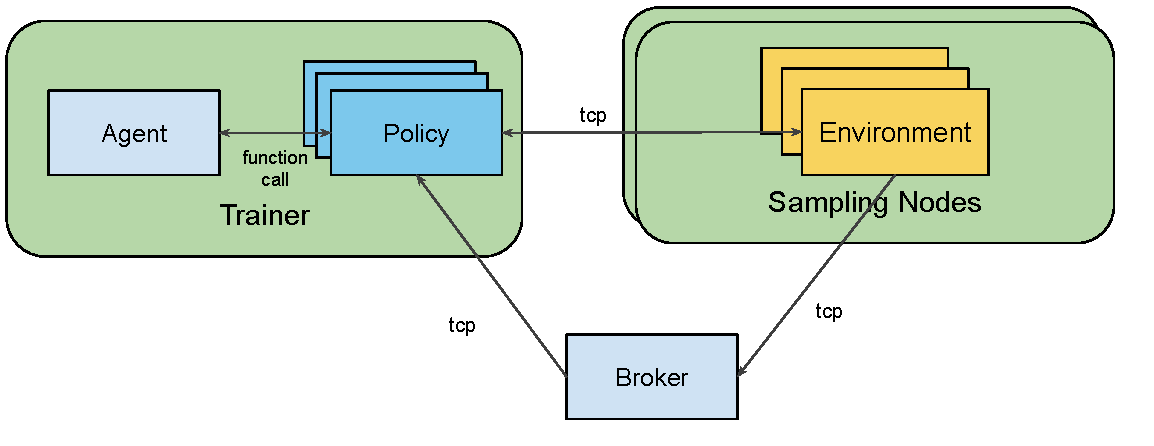
\includegraphics[width=0.7\textwidth]{images/Distributed-QBlade.pdf}
  \caption{A schema of the distribution framework. Environments can be placed on different nodes than the node the training is running on}
  \label{fig:distributed-framework}
\end{figure}

This asynchronous reset is the main idea constituting our framework for distributed wind turbine reinforcement learning \cite{westerbeckFrameworkDistributedWind2021}. Figure \ref{fig:distributed-framework} outlines this concept. Environments are process-separated from the sampling policy and communicate via tcp. This enables placement of environments on multiple sampling nodes, which can be different to the node of the sampling policy. The individual nature of the environments further allows them to reset asynchronously, as for the reset, no policy input is needed. The connection is established after a successful reset with the help of a \textit{broker} component, which keeps track of the state and tcp address of all environments and hands out a ready environment to requesting policies. 

It is possible to scale the amount of environments past the amount of sampling policies in our framework, effectively enabling a total speed-up factor up to the ratio of reset time to sampling time. As some simulation configurations need a reset time equal to the sampling time, we could measure a factor two speed-up over the default distributed sampling implementation by garage. All tcp connections are wrapped with ZeroMQ, enabling a fault-tolerant training process, and serialization is performed through protobuf, a high-speed and language agnostic serialization protocol.

Further improvements include changes to the multiprocessing sampler. The garage implementation offers an inefficient sampling stop condition. The sampler keeps starting new rollouts until the desired amount of environment interactions has been recorded. For example, if eight workers collect rollouts in parallel and seven of these finish, the stop condition has not been reached. Hence, all seven workers are instructed to collect another rollout. When the slowest worker finishes the first rollout shortly after, the stop condition is reached and sampling stops. Problematically, the seven other workers have already allocated an environment. They discart their allocation, and the environment has to reset. This behavior is acceptable for environments with short reset times, but for wind turbine environments with long reset times, this is a major performance loss. Changing this behavior has lead to another measured speed-up factor of almost two.

To perform grid searches, we investigated the hyperparameter tuning framework ray tune by \citet{liawTuneResearchPlatform2018}. Ray tune implements several sophisticated hyperparameter search algorithms and promises easy integration into any machine learning setup. However, we observed problematic behavior due to the fact that both ray tune and garage utilize the distributed python library ray. Ray spawns a number of components each time it is used, including a redis instance and several worker and watchdog processes. When combining the two frameworks and scaling them to a decent extent, the resulting utilization of unix processes and tcp ports exceeds the possibilities of the linux operating system on the cluster. The default reaction of linux is to fail the fork operation or socket allocation, which immediately crashes the training process and the involved ray worker. To make matters worse, ray workers are self-healing, means if a worker is missing, it is respawned immediately. In this case, this meant that the processes killed by the operating system would be restarted immediately by ray. We were unable to manually kill ray processes as fast as ray respawned them, normal interaction with the ray cluster was broken due to the tcp port exhaustion, and the operating system was unresponsive due to the accidental fork bomb. Hence, we implement our own grid search framework based on pythons inbuilt multiprocessing capabilities.
  

\subsection{Hyperparameters}
\label{section:approach-hyperparameters}

\begin{summary}
The choice of hyperparameters is a significant success factor to machine learning in general. This subsection presents a table of hyperparameters and describes our process of hyperparameter choice. In addition, we present the intuition behind hyperparameter effects for some hyperparameters. Because of space constraints, we can not include the entire experimentation performed to obtain these values. However, we include grid searches for a selection of hyperparameters in the results chapter.
\end{summary}

In Table \ref{table:hyperparameters}, hyperparameters and their default values for each wind scenario are listed. We require different hyperparameters for the different wind scenarios as the challenges associated with each scenario are different. The steady wind has a fully deterministic dynamic where subtle changes in the policy have a great impact, while the turbulent wind is dominated by the unpredictable nature of the wind inflow. These defaults form a basis for obtaining solid training results. When we deviate from these hyperparameters in the results section, we denote these deviations.

\newcommand\hparam[4]{#4 & $#1$ & #2 & #3  \\}
\begin{table}
  \centering
  \begin{longtable}{lccc}
    \toprule
    Description & Symbol & Steady & Turbulent \\
    \midrule
    \hparam{\targetupdate}{0.995}{0.995}{Smooth target update coefficient}
    \hparam{\gamma}{0.98}{0.99}{Discounting factor}
    \hparam{}{tanh}{tanh}{Activation function of the policy MLP}
    \hparam{}{256, 256}{256, 256}{Sizes of the hidden layers of the policy MLP}
    \hparam{}{tanh}{tanh}{Activation function of the Q function MLP}
    \hparam{}{256, 256}{256, 256}{Sizes of the hidden layers of the Q function MLP}
    \hparam{}{3e-5}{1e-5}{Learning rate of the policy}
    \hparam{}{3e-4}{1e-4}{Learning rate of the Q function}
    \hparam{\alpha_0}{0.05}{0.2}{Initial policy standard deviation}
    \hparam{\targetentropy}{-20}{-20}{Target entropy}
    \hparam{}{16000}{24000}{Number of environment interactions per epoch}
    \hparam{\lambdatraj}{2000}{2000}{Maximal trajectory rollout length}
    \hparam{}{200}{200}{Number of gradient descend steps per epoch}
    \hparam{}{256}{256}{Training batch size}
    \hparam{}{2e6}{2e6}{Maximum replay buffer size}
    \hparam{}{16e4}{16e4}{Minimal replay buffer size before commencing training}
    \hparam{\lambdaspat}{0.01}{0.2}{Spatial regularization coefficient}
    \hparam{\lambdatemp}{0.05}{0.2}{Temporal regularization coefficient}
    \hparam{\epsspat}{0.1}{0.1}{Spatial regularization standard deviation}
    % \hparam{\drrrcoeff}{0}{DR3 regularization coefficient}
    \hparam{\lambdapast}{6}{6}{Dilated past feeding steps}
    \hparam{\rcoleman}{2e-7}{2e-7}{Reward blade bending penalty}
    \hparam{\rconst}{1}{1}{Reward function constant offset}
    \hparam{\rcolemanact}{0}{0.02}{Reward pitch travel penalty}
    \hparam{}{$\pm$5}{$\pm$5}{Reward clipping range}
    \midrule
    \hparam{}{false}{true}{Allow $c_S$ action control}
    \hparam{\ipcplay}{$\pm$ 3}{$\pm$ 4}{IPC control play [deg]}
    \hparam{}{$\pm0.5$}{$\pm0.5$}{$\philead$ control play [rad]}
    \hparam{\tauhp}{$1/0.2$}{$1/0.2$}{Preprocessing high-pass filter tau}
    \hparam{\pitchmodelfreq}{$4\cpi$}{$4\cpi$}{Pitch actuator model frequency}
    \hparam{\pitchmodeldamp}{0.7}{0.7}{Pitch actuator model damping coefficient}

    \bottomrule
  \end{longtable}
  \caption{Table of hyperparameters with their symbol, default value and a description}
  \label{table:hyperparameters}
\end{table}

We found some hyperparameters to have a higher impact than others, among the most important ones being $\lambdatemp, \lambdaspat$. $\lambdatemp$ and $\lambdaspat$ modify the smoothness of the policy and have a high impact on pitch actuator wear. The smoother a policy is, the less pitch actuator wear it induces. Furthermore, they also have an impact on blade actuator wear, as a smoother policy also protects the blades, especially in the steady wind. 

$\gamma$ controls how strongly rewards far in the future are discounted, meaning how much influence they still have currently or how short-sighted optimization should be. In our case, this affects the relation of the reward function to the actual wear metrics. With a lower $\gamma$, the term minimizing pitch wear has a higher effect on pitch wear, while with a higher $\gamma$, the blade wear term is more effective. We credit this to the learnability of these functions, as blade wear is more difficult to learn than pitch wear. With a lower $\gamma$, the blade wear term is mainly noise, as most of the blade wear is induced by the wind. Only over longer periods of optimization, the difference another policy can have on blade wear becomes clear.

The number of environment interactions per epoch controls how often gradients are calculated. With 16000, we chose a value much higher than the \ac{SAC} defaults. While we found this to slightly hurt the number of epochs required to convergence, it did not significantly hurt final policy performance. With a higher number of environment interactions per epoch, we can parallelize the sampling process better. In this case, eight environments can sample in parallel, which results in a drastic reduction in wall-clock time. Further increasing the amount of steps per epoch yielded performance improvements that did not justify the additional compute budget anymore.

Initial policy standard deviation (also called initial temperature coefficient) $\alpha_0$ and target entropy $\targetentropy$ relate to the option of \ac{SAC} to control entropy in the maximum-entropy RL setting. During training, $\alpha$ will slowly approach $\targetentropy$ in an exponential decay pattern. For the wind turbine, choosing a low $\targetentropy$ means the policy will have minimal noise at the end of the training process. Some noise is required to ensure exploration, especially at the beginning of the training, so the starting entropy is a little higher. We tuned both parameters to the lower limit that would still allow stable training.

The activation functions are specified to be ReLU in the \ac{SAC}-paper, but we use tanh in our work. The difference between the two is minimal, but tanh yields slightly smoother policies in our experiments. As the networks are relatively shallow, typical problems with sigmoid-like activations like vanishing gradients on saturated activations or activation drift do not play out detrimental.

The size of the neural networks specifies the potential to learn complex functions. More parameters generally mean more difficult functions can be learned. In general machine learning, the number of parameters in a neural network can be used to control the bias-variance trade-off. In reinforcement learning, the bias-variance trade-off is not a big concern yet, as biases induced through the Bellman backup or other training techniques usually exceed approximation errors due to underparametrization \cite{fujimotoAddressingFunctionApproximation2018}. Consequently, minimizing bias is the primary aim, and the downside of high-variance estimators can be ignored by not benchmarking generalization \cite{cobbeQuantifyingGeneralizationReinforcement2019}. For more complex types of neural networks such as convolutional networks, a higher number of layers boosts training performance, but for a \ac{MLP}, the number of layers does not matter. Given enough neurons per layer, any function can be approximated with just two layers. With these considerations in mind, we found two layers with 256 neurons to work well; adding more neurons did not improve performance.

The training batch size is another parameter that is used to control the bias-variance trade-off in traditional machine learning. The smoothing effect of high batch sizes can be used to limit variance while loosing fine fit. Furthermore, high batch sizes improve GPU efficiency. Our cluster does not have GPUs and the bias-variance trade-off is not a major concern, so we utilize the default batch size from \ac{SAC}.

The learning rate is a parameter, which has a major impact in supervised learning. It dictates how far to make a gradient step, with too low values resulting in long trainings and high susceptibility to local maxima, and too high values in loss explosions and coarse fit. In reinforcement learning, a non-stationary quantity is subject to optimization. The Q-function targets change with policy performance and Q-function fit, hence a complex interaction of policy and Q-networks emerges, which makes the choice of learning rate non-trivial. \citet{kakadeNaturalPolicyGradient2001} prove that second-order optimization over the environment dynamics can find a sensible step size for each gradient, however \ac{SAC} uses first-order optimization only. Resultingly, the learning rate has to be sufficiently small to avoid catastrophic steps and detrimental interactions between policy and Q optimization. Furthermore, the dynamic between policy and Q-function is complex to control. We found a policy learning rate one magnitude smaller than the Q learning rate to stabilize trainings, as the Q estimates have time to settle to the current policy performance before the policy changes too drastically.

Finding the best hyperparameters for a machine learning algorithm is a non-trivial task, and automatizing this task forms a separate field in machine learning called \textit{AutoML} \cite{hutterAutomatedMachineLearning2019}. We chose to optimize our hyperparameters through \textit{grid search}, which means to run a full training for every sensible combination of hyperparameters. As we lack the computation resources to perform a full grid search over all hyperparameters, we pair grid searches over small subsets of the hyperparameter space with \textit{grad student descend} \cite{gencogluHARKSideDeep2019}, a methodology where a student tries hyperparameter subsets until it works.


\subsection{Evaluation Methodology}
\label{section:approach-evaluation-methodology}

\begin{summary}
This subsection describes the evaluation procedures and metrics used, comparison baselines, and the exact procedure for calculating metrics. Our baselines are a \ac{CPC} and a \ac{IPC} control strategy, with our main metric being DELs, a metric for component wear. 
\end{summary}

\subsubsection{Baselines}

We use two validated controllers as a reference baseline. One is a \acf{CPC} as described in \cite[Section 3.2.1]{perez-beckerImplementationValidationAdvanced2021}. It integrates state-of-the-art features such as gain scheduling, notch-filtering drivetrain eigenfrequencies, and techniques to prevent integrator saturation. Its parameters were tuned to the IEA 10MW turbine by an expert for wind turbine control. Furthermore, we use a second baseline which implements an \acf{IPC} as described in \cite[Section 3.2.2]{perez-beckerImplementationValidationAdvanced2021}. We outline the properties of this strategy in our background Section \ref{section:background-ipc}. Similar to the \ac{CPC}, parameters were tuned to the IEA 10MW turbine by an expert for wind turbine control.

\subsubsection{Procedures}

Garage offers inbuilt evaluation capabilities. After each epoch, the algorithm can be evaluated in a separate evaluation environment. This inbuilt evaluation phase offers no distribution option, and it is difficult to extract and save collected evaluation rollouts for further inspection. We implement a separate evaluation phase which runs in a dedicated Slurm job. The configuration of our evaluation environments is different to the training configuration. Hence, separating the evaluation phase to another job results in better hardware utilization, as only the type of environments which is in use is spawned.

While our training takes place in randomized environments, we utilize deterministic settings for the simulation in the evaluation phase. For tracking our training progress, each checkpoint is evaluated in eight deterministic environments. From this, metrics are accumulated to form training plots. For a detailed evaluation of a single checkpoint, we utilize a higher number of deterministic environments. In the steady wind setting, we evaluate the wind range in 0.1 m/s steps. In the turbulent setting, we evaluate in 0.2 m/s steps with eight turbulence seeds for each wind speed. To allow for a direct comparison of policy performance, the baseline \ac{CPC}, the baseline \ac{IPC}, and our neural controller are run on each of the environments.

We observed slightly better results with deterministically evaluated policies compared to using the stochastic policy directly. Hence, we evaluate our trained policies deterministically for the entire evaluation: $\pi_{\text{det}}(s) = \argmax_{a} \pi(a|s)$. As the output of the policy is a multivariate Gaussian, the argmax operation is implemented by taking the mean of the Gaussian as action output. Through both a deterministic policy and a deterministic environment, the evaluation rollouts are deterministic and can be compared directly. Unless stated otherwise, we utilize the highest performing policy of a training run, which not necessarily the last iteration.

As recommended in \citet{agarwalDeepReinforcementLearning2022}, we use the \acf{IQM} method for mean estimations that are robust to outliers in most of this work. The \ac{IQM} of a set of values is computed by discarting the lowest 25\% and highest 25\% of all elements and computing the arithmetic mean across the remaining elements. For example, the values $\{1, 1.1, 1.3, 4.7\}$ are pruned to $\{1.1, 1.3\}$ and then averaged to an IQM of 1.2. The values can be of any metric for which a traditional arithmetic mean can be calculated.

\subsubsection{Metrics}

While reward is the quantity subject to optimization, we utilize further metrics to improve interpretability of our results.

As additional evaluation metrics, we calculate \acp{DEL} as outlined in Section \ref{section:damage-equivalent-loads} for \ac{BRBM} and for pitch actuation. For brevity, we denote \ac{bDEL} as the \ac{DEL} metric for \ac{BRBM} and \ac{pDEL} for pitch actuation. We use the python framework \textit{rainflow} for rainflow calculation, which we found to deliver reasonably close results to those of \textit{Crunch} \cite{buhlCRUNCHUSERGUIDE2001}, a widely validated and adopted tool which supports Rainflow counting. We bin to n=128 bins, cohering to the default settings of Crunch. For calculating \acp{bDEL}, we use a Wöhler exponent $\woehler = 10$ which is typical for glass fiber and a \ac{DEL} frequency $\fdel = 1$ Hz. Furthermore, we average \acp{bDEL} of the three individual blades into one value. The resulting formula is shown in Equation \ref{eq:bdel}:

\begin{equation}
  \bdel = \frac{1}{3} \sum_{i \in {1,2,3}}(\del(\trajectory_{\soopbend_i}, \woehler=10, \fdel=1))
  \label{eq:bdel}
\end{equation}

where $\trajectory_{\soopbend_i}$ denotes the bending moment signal of blade $i$ along the entire trajectory $\trajectory$. For \acp{pDEL} $\pdel$, the DEL metric of the pitch signals, we use $\woehler = 1$ and $\fdel = 1$ Hz. We average the resulting \ac{pDEL} values across all blades, as in Equation \ref{eq:pdel}:

\begin{equation}
  \pdel = \frac{1}{3} \sum_{i \in {1,2,3}}(\del(\trajectory_{\spitchx_i}, \woehler=1, \fdel=1))
  \label{eq:pdel}
\end{equation}

with $\trajectory_{\spitchx_i}$ denoting the pitch actuation signal of blade $i$ along the trajectory. To calculate an improvement, we divide the reinforcement learning results by the results obtained by running the baseline \ac{IPC} on the same simulation setting: $\delrel = \frac{\del_{rl}}{\del_{ipc}}$. Values of $\delrel<1$ mean the learnt policy performs better than the baseline \ac{IPC}, in the sense of creating less \ac{DEL}. 

% Finally, a weighted DEL metric \textit{wDEL} which combines the relative pitch \ac{pDEL} $\pdelrel$ with the relative blade \ac{DEL} $\bdelrel$ can be computed as $\wdel(\pbtrade) = \pbtrade \bdelrel + (1-\pbtrade) \pdelrel$. The pitch-blade trade-off factor $\pbtrade \in [0,1]$ determines the relative importance of reducing blade bendings versus reducing pitch actuation. This trade-off factor is to be determined for each turbine, and is affected by a variety of engineering constraints such as parts cost, lifetime, and wear resilience. A factor $\pbtrade > 0.5$ means lowering $\pdel$ is more important than lowering $\bdel$, and vice versa. Hence, an RL policy, which reduces bending moments while increasing pitch actuation, is still evaluated as an improvement over the baseline if the pitch actuation increase is outweighed.

In the turbulent wind setting, extreme loads also play a role. In contrast to fatigue loads, the number of cycles can be minimal to cause damage to the blade. Albeit DELs capture the full load range, the metric exhibits inaccuracies on extreme values. Hence, we quantify them separately with the 99\% quantile value of blade bending moments. The pitch actuator does not require an extreme load analysis, as the pitch actuator is more susceptible to wear through high and fast pitch travel than to high pitching amplitude.

To qualitatively analyze behavior, we use the visualization tool \acf{PSD} plot. These plots show the spectral activity of a time series. They have the frequency spectrum on the x-axis and the intensity of activity on that frequency on the y-axis. In our work, we utilize log-scales for the y-axis to facilitate readability. They are computed by Fourier-transforming the time series and then summing the frequency contents of the Fourier-transformed signal across the time axis. A pure sine wave would show as a single excited frequency in the Fourier-transformed signal, as a horizontal line in a spectogram, and as a single peak in a \ac{PSD} plot. If there are peaks on exact multiples of a frequency, these multiples are called \textit{harmonic frequencies}.


\chapter{Results}
\label{ch:results}

This chapter contains the validation of \ac{WINDL}. For this work, two fields of research have been combined, wind turbine load control and reinforcement learning. The two fields have different metrics and evaluation focus. We incorporate both focus points into this chapter, dedicating each section to a specific perspective.

We split the bigger problem of wind turbine load control by looking at different wind scenarios. As explained in Section \ref{section:background-optimization-aims}, we split the incoming wind into an easier steady wind scenario and the more unpredictable turbulent wind scenario. Furthermore, we evaluate different wind speeds for both wind scenarios. As explained in Section \ref{section:background-wind-turbine-fundamentals}, two control policies are switched at rated speed. While we are mostly interested in the above-rated regimes, the transition period is of interest as well. The following sections utilize mainly wind turbine load control evaluation methodology:

\begin{enumerate}
  \item Section \ref{section:results-steady-fatigue} evaluates \ac{WINDL} with respect to fatigue loads in the steady wind.
  \item Section \ref{section:results-transition} evaluates the transition period around rated speed in the steady wind.
  \item Section \ref{section:results-naive-turbulent} evaluates the unadjusted \ac{WINDL} in the turbulent wind scenario.
  \item Section \ref{section:results-adjusted} evaluates an adjusted version of \ac{WINDL} in the turbulent wind scenario.
\end{enumerate}

While the final policy performance is better to be evaluated through the lens of wind turbine load control, problems and adjustments require the evaluation methodology of reinforcement learning. While reinforcement learning generally offers great flexibility and requires little algorithmic changes to optimize arbitrary problems, it has drawbacks when it comes to interpretability, generalization, and robustness. The following sections address challenges in the reinforcement learning perspective:

\begin{enumerate}
  \item Section \ref{section:results-pb-trade-off} addresses a fundamental trade-off in wind turbine control through choice of hyperparameters.
  \item Section \ref{section:results-transfer} investigates generalization performance from one wind setting into the other.
  \item Section \ref{section:results-reward} analyzes the performance of the reward function
  \item Section \ref{section:results-rl-components} shows the interaction of different components in the RL algorithm.
\end{enumerate}


\section{Steady Wind Fatigue Loads}
\label{section:results-steady-fatigue}

\begin{summary}
In this section, we demonstrate that WINDL produces lower fatigue loads than state-of-the-art baseline controllers in the steady wind scenario above rated speed. We first measure pitch and blade fatigue loads across all wind speeds above rated speed and then investigate the different policy behaviors to understand how WINDL outperforms current baselines. We find that pitch activity on multiple frequencies is a major cause for the improved policy performance.
\end{summary}

For this section, we utilize hyperparameters as in Section \ref{section:approach-hyperparameters} and evaluation methodology as in Section \ref{section:approach-evaluation-methodology}. We train 12 experiments with different random seeds for 750 epochs (approx. 10M environment interactions) and choose the best result among them for presentation.

As described in Section \ref{section:background-optimization-aims}, the steady wind setting is a scenario in which the wind speed does not change over time. There is a wind shear present, meaning there is a change in wind speed over height with higher speeds further up and lower speeds further down in the boundary layer. Because of this shear, the optimal control policy is a cyclic policy, which repeats every revolution of the rotor, as the wind conditions are exactly the same after every full rotation. A constant control policy like the \ac{CPC} is not optimal with respect to blade bending moments as it does not account for the different wind speeds a blade experiences across a single rotation. Power production above rated is not a concern, as the generator runs at rated power with the pitch controller limiting aerodynamic torque generation to the rated maximum.

\subsection{Presentation}

\begin{figure}
  \centering
  \begin{subfigure}[b]{0.48\textwidth}
      \centering
      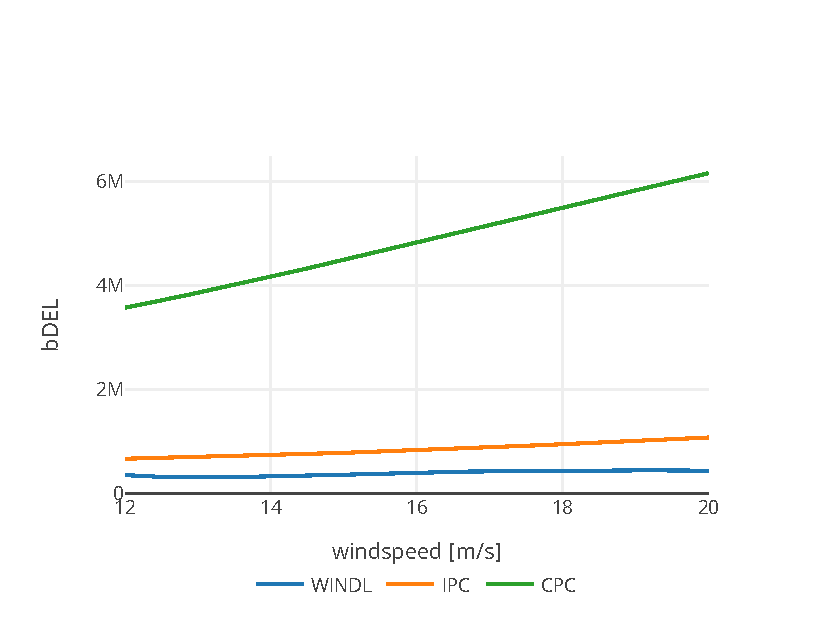
\includegraphics[width=\textwidth]{images/steady_sweep_bdel.pdf}
      \caption{blade-\ac{DEL} against windspeed}
      \label{fig:steady-sweep-bdel}
  \end{subfigure}
  \begin{subfigure}[b]{0.48\textwidth}
      \centering
      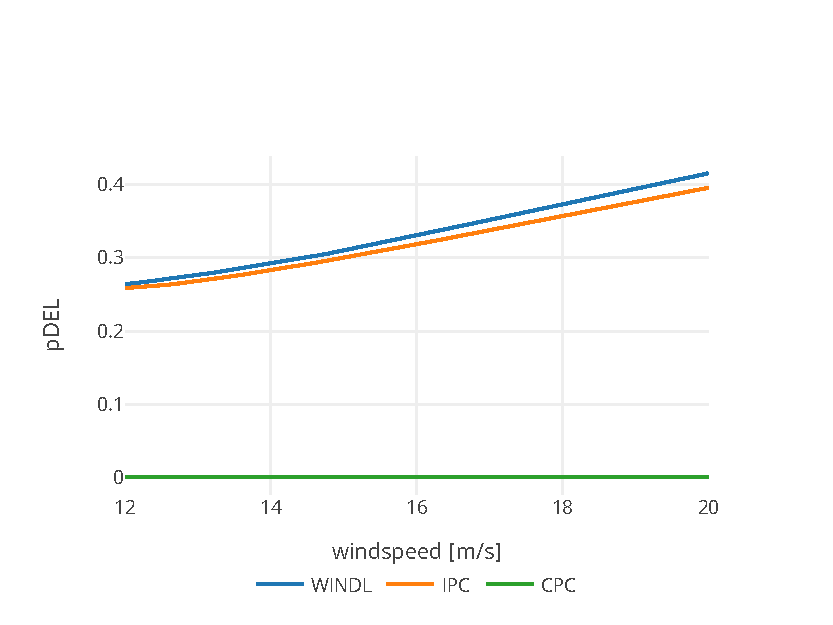
\includegraphics[width=\textwidth]{images/steady_sweep_pdel.pdf}
      \caption{pitch-\ac{DEL} against windspeed}
      \label{fig:steady-sweep-pdel}
  \end{subfigure}
  \caption{bDEL and pDEL metrics for the above-rated operation regime, lower is better. The WINDL controller outperforms both controllers with respect to bDEL, while having a slight hit to pDELs.}
  \label{fig:steady-sweep}
  % sac-steady-final, data_0, reeval_468
\end{figure}

Figure \ref{fig:steady-sweep} shows the evaluation metrics bDEL in \ref{fig:steady-sweep-bdel} and pDEL in \ref{fig:steady-sweep-pdel} for all wind speeds in the above-rated operating regime from 12 to 20 m/s with a resolution of 0.1 m/s, evaluated for the three control policies CPC, IPC, and WINDL. As all control policies and the environment are deterministic, we evaluate a single run for each wind speed. The CPC policy exhibits high bDEL moments but pDEL moments of zero in the steady regime, as it keeps the pitch angles constant. IPC and WINDL both outperform the CPC in terms of DEL moments, as they both employ a policy to account for the wind-shear, but induce pitch actuator wear. The DEL moments induced by WINDL are on average 54.1\% below those of the IPC and 92.0\% below those of the CPC, bringing a significant advantage in blade fatigue wear in comparison to both baselines. This comes at the price of an average of 3.8\% higher pDEL than the IPC.

\subsection{Investigating Policy Actions}

\begin{figure}
  \centering
  \begin{subfigure}[b]{0.48\textwidth}
      \centering
      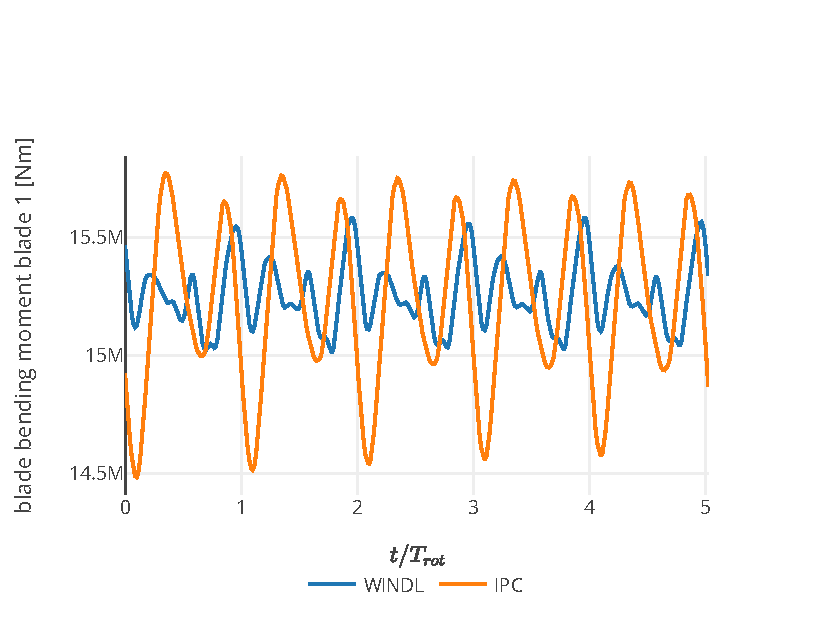
\includegraphics[width=\textwidth]{images/steady_rollout_blade_bending.pdf}
      \caption{Blade bendings against rotor revolutions}
      \label{fig:steady-rollout-blade-bending}
  \end{subfigure}
  \begin{subfigure}[b]{0.48\textwidth}
      \centering
      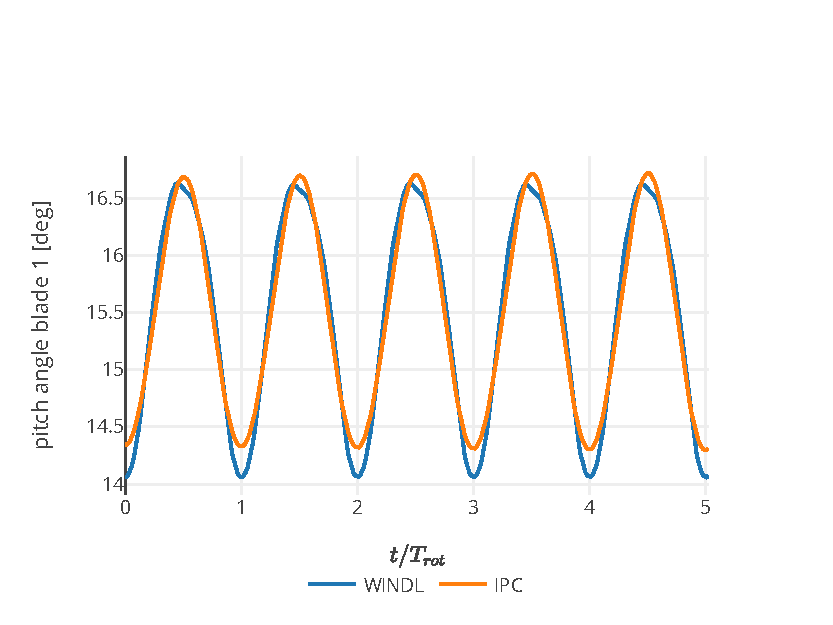
\includegraphics[width=\textwidth]{images/steady_rollout_pitch.pdf}
      \caption{Pitch actuation against rotor revolutions}
      \label{fig:steady-rollout-pitch}
  \end{subfigure}
  \begin{subfigure}[b]{0.48\textwidth}
    \centering
    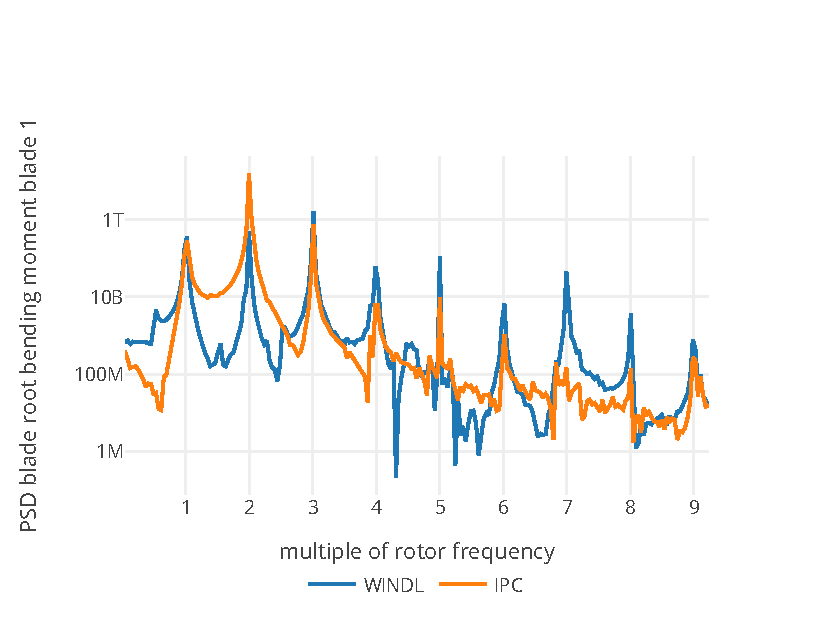
\includegraphics[width=\textwidth]{images/steady_rollout_blade_psd.pdf}
    \caption{Power spectral density plot for blade root bending moments}
    \label{fig:steady-rollout-blade-psd}
  \end{subfigure}
  \begin{subfigure}[b]{0.48\textwidth}
    \centering
    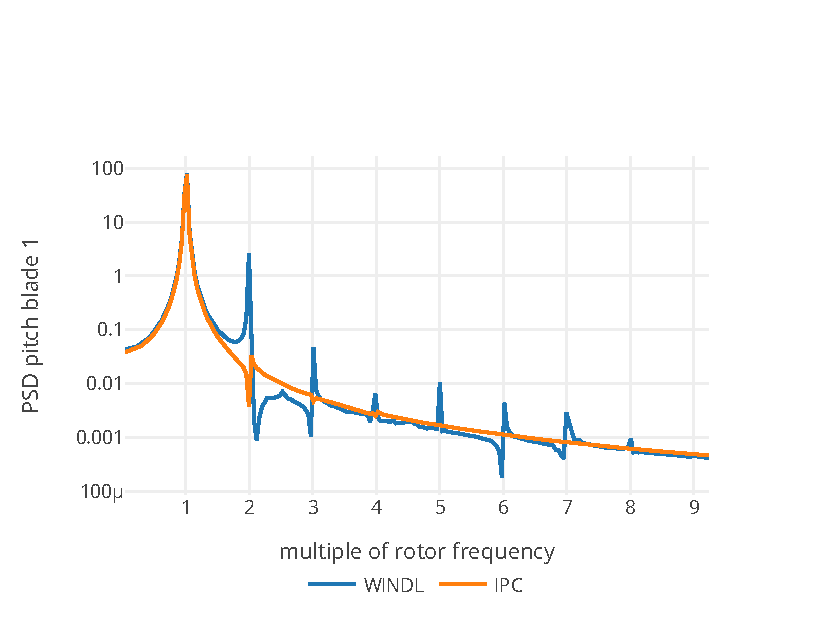
\includegraphics[width=\textwidth]{images/steady_rollout_pitch_psd.pdf}
    \caption{Power spectral density plot for pitch actuation}
    \label{fig:steady-rollout-pitch-psd}
  \end{subfigure}
  \caption{Detailed comparison of WINDL and IPC control policies at a wind speed of 18 m/s. The WINDL policy actuates on a higher number of frequencies, counteracting vibrations on more than the base rotor frequency}
  \label{fig:steady-rollout}
  % sac-steady-final, data_0, reeval_468, run 80 windspeed 18m/s
\end{figure}

To understand how the WINDL controller is able to achieve such a significant improvement, Figure \ref{fig:steady-rollout} compares the WINDL and IPC strategies in detail for a single blade and on a single wind speed of 18 m/s. Bending moments, pitch actuation, and \ac{PSD} for the other two blades are omitted, as they exhibit similar behavior with a delay of a third of a rotation and as such do not provide further information for a qualitative analysis. Other wind speeds are also omitted, as they mainly change the magnitude of pitch actions and blade bendings, not their nature. The wind speed of 18 m/s is chosen as a representative as it most clearly shows the differences between \ac{WINDL} and the IPC baseline. Subplot \ref{fig:steady-rollout-blade-bending} shows the blade root bending moments over rotor revolutions for blade 1. A pattern which repeats every revolution is visible for both policies. Because the inflow conditions are steady, the turbine state is equal every 360 degrees of rotation and a together with a damping control policy, vibrations are constant. Note that we did not explicitely constrain WINDL to have a damping effect, it learned this purely by optimizing the reward function. While the arithmetic mean of the bending moments differ only by 0.1\% between WINDL and IPC, bending moment oscillations induced by the WINDL controller are significantly smaller in amplitude. This smaller amplitude is the driving factor for the bDEL reduction. The relatively small difference in pDELs is caused by a small difference in pitch amplitude, as shown in Subplot \ref{fig:steady-rollout-pitch}. The significant difference between the policies lies in the rich spectral content of the WINDL pitch actuation, as shown in Subplot \ref{fig:steady-rollout-pitch-psd}. While having similar actuation on the 1p frequency, the WINDL controller acts significantly more on the 2p frequency with actuation peaks all the way up to 8p. Especially the effect of the actuation on the 2p frequency shows in the bending moment \ac{PSD}-plot in Subplot \ref{fig:steady-rollout-blade-psd}. At this frequency, WINDL achieves ca. 30 times lower bending oscillation amplitude than the IPC (note the log scale). Even though WINDL exhibits partially higher amplitudes on higher frequencies, this does not offset the saving around 2p.

\subsection{Discussion}

We show WINDL to produce significantly lower fatigue loads than state-of-the-art baseline controllers in the steady wind scenario at the expense of a slight increase in pitch actuation, offsetting the current state-of-the-art by 54.1\%. Instead of trading pDEL for bDEL directly, WINDL actuates with richer spectral contents, achieving a significant bDEL decrease at the cost of just 3.8\% higher pDEL. This shows that WINDL has the potential to match or even outperform state-of-the-art control systems in chosen metrics by black-box optimization only, without requiring information about the underlying physical processes of the environment. 

Albeit the reward function does not incentivize pitch wear reduction ($\rcolemanact=0$), the policy does not trade pitch wear excessively. We attribute this to the smoothness regularization, which smoothes the policy to lower pitch fluctuation. While in theory, further blade wear reductions could be possible by increasing pitch activity on higher frequencies, our pitch actuator model does not support much more activity on high frequencies. Hence, we believe this performance to be close to the optimal performance possible in the steady wind for the given turbine, so WINDL has no reason to increase pitch activity.

The IPC limits its activity to the 1p frequency, whereas WINDL pitches on all frequencies up to 8p. Note that we did not specifically incentivize the rich spectral content; it is purely emerging from black-box optimization given the environment and the reward function. This supports recent findings from traditional wind turbine research, specifically of \citet{vansolingenLinearIndividualPitch2015} which propose a 1p-2p-3p linear pitch controller. In traditional controller design, frequencies above 3p are often disregarded due to the small influence they have on the end result. Also, not every pitch actuator is capable of reproducing such high frequencies. For the IEA-10MW turbine, the 1p rotation frequency corresponds to 0.14 Hz, hence 8p would be at around 1.15 Hz. Oscillating the massive 48 ton blades at this frequency is at the limits of physically possible. However, for the simplistic actuator model used in this work, it seems to play out favorably to pitch on such high frequencies. These experiments show that black-box optimization through WINDL can be used to reinforce and improve scientific understanding in the field of wind turbine control.

Depending on the turbine and operating site, the \ac{LCOE} can benefit differently from component load relief. A turbine model can have sensitive blades and require the maximum possible blade wear relief, or be more sensitive to pitch wear. Currently, the IPC policy is commonly used on turbines that benefit from blade load reductions past the capabilities of a CPC. With our findings, we show that the \ac{WINDL} policy could be a good fit for such situations as well, providing further blade load relief than the IPC policy. Our strategy extends the range of options for wind turbine manufacturers and operators to choose the best possible strategy for their turbine.

\section{Transition Around Rated Wind Speed}
\label{section:results-transition}

\begin{summary}
In this section, we demonstrate that WINDL produces lower fatigue loads at the cost of power around rated speed in the steady wind scenario. We measure blade fatigue loads and power production around rated speed and then follow up with two rollouts. Along with the rollouts, we investigate a phenomenon where WINDL utilizes the individual blades very unevenly below rated speed.
\end{summary}

For this section, we evaluate the same model as in Section \ref{section:results-steady-fatigue} in wind speeds between 10 and 12 m/s around the rated wind speed of the turbine.

The transition period around rated speed poses significant challenges in wind turbine control due to two major reasons, high thrust and controller design. The aerodynamic thrust on the rotor is at its maximum at rated (see Figure \ref{fig:IEA10MW}), as the regulation of the pitch controller above rated speed decreases rotor thrust faster than the increase in wind speed can increase thrust. Hence, the turbine is especially susceptible to extreme loads in this operating range. Furthermore, controller design theory works with a switch in control systems at rated speed. Below rated, the torque controller regulates the turbine, and above the pitch controller does. This leaves the question open to what happens \textit{at} rated speed, and current methods mainly focus on getting the policy switch to work without having a specific optimization criterium in mind \cite[Section 8.3.4]{burtonWindEnergyHandbook2011}. 

\subsection{Presentation}

\begin{figure}
  \centering
  \begin{subfigure}[b]{0.48\textwidth}
      \centering
      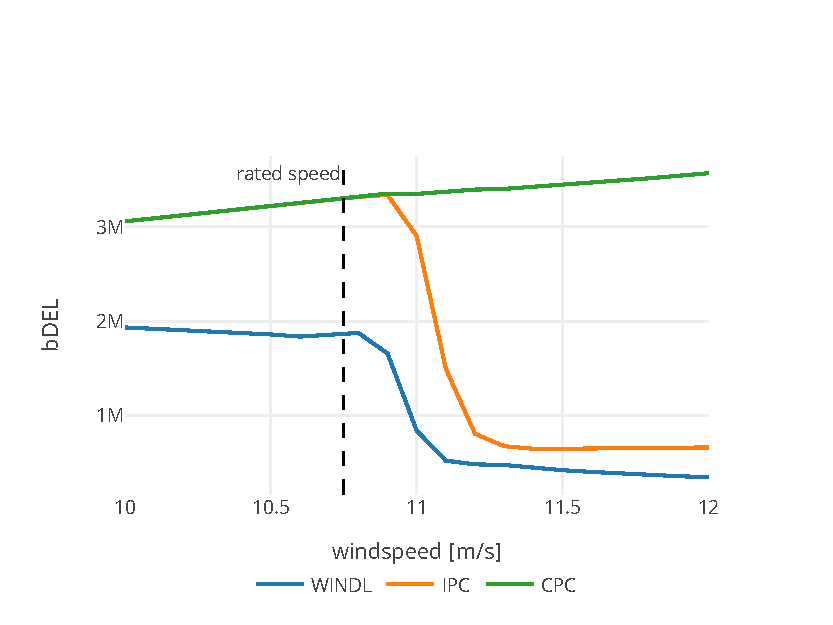
\includegraphics[width=\textwidth]{images/transition_bdel.pdf}
      \caption{Blade-\ac{DEL} against windspeed}
      \label{fig:transition-bdel}
  \end{subfigure}
  \begin{subfigure}[b]{0.48\textwidth}
      \centering
      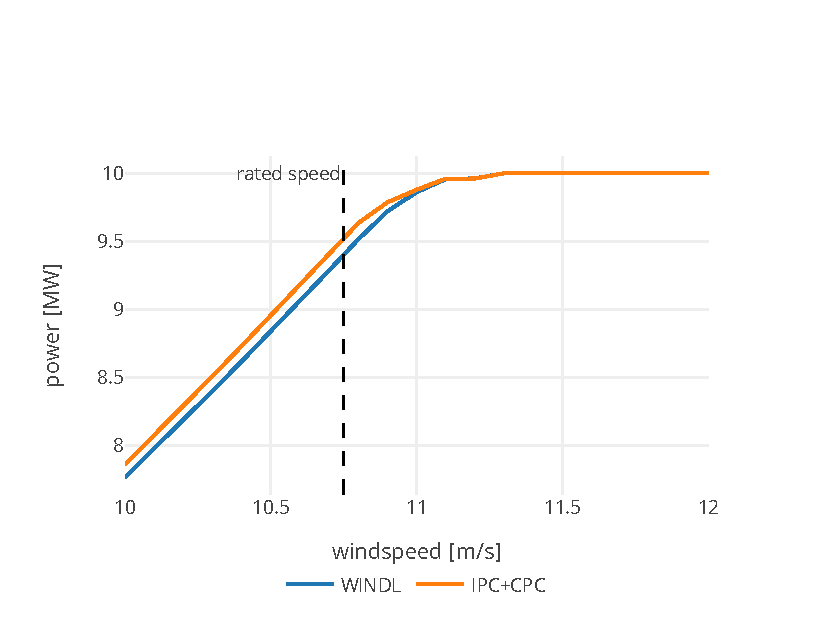
\includegraphics[width=\textwidth]{images/transition_power.pdf}
      \caption{Average power production against windspeed}
      \label{fig:transition-power}
  \end{subfigure}
  \caption{Blade-DEL and power production against windspeed in the transition period around rated speed. WINDL offers significantly lower blade DELs at the cost of some power loss.}
  \label{fig:transition}
  % sac-steady-final, data_0, reeval_468 
\end{figure}

Figure \ref{fig:transition} shows the bDEL metric and average power production for CPC, IPC, and WINDL control policies. The rated speed of the IEA-10MW turbine is indicated by a dashed line at 10.75 m/s. In \ref{fig:transition-power}, the power curve of CPC and IPC are exactly equal. This is due to the IPC being designed such that it ramps down its activity at slightly above rated speed before any power is lost \cite{perez-beckerImplementationValidationAdvanced2021}. For the IEA-10MW turbine, the ramp-down is scheduled between 11.2 and 10.9 m/s, as visible in the IPC curve in \ref{fig:transition-bdel}. WINDL exhibits a power reduction of 1.23\% at rated speed, or 0.62\% reduction averaged across the shown transition period of 10 m/s to 12 m/s. In turn, it achieves a bDEL reduction of 42.9\% compared to the IPC baseline, and 64.1\% compared to the CPC baseline across the transition period. 

Both WINDL and the IPC experience a sharp increase in bDEL for small decreases in wind speed around 11 m/s. For WINDL, bDELs jump up from 0.42M at 11.5 m/s to 1.71M at rated speed, for the IPC they jump from 0.65M at 11.5 m/s to 3.3M at rated speed. Such a sharp increase is the result of two phenomena occurring in parallel, maximal rotor thrust and minimal pitch activity. For the IPC, this is exacerbated by the activity ramp-down, which transitions into a CPC policy at rated. For WINDL, the sinusoidal motion, which is possible above rated, is cut off below rated due to the cap in pitch angle at 0 degrees. This introduces the need for a different policy at rated speed. 

\subsection{Different Blade Action Phenomenon At Rated Speed}

\begin{figure}
  \centering
  \begin{subfigure}[b]{0.48\textwidth}
      \centering
      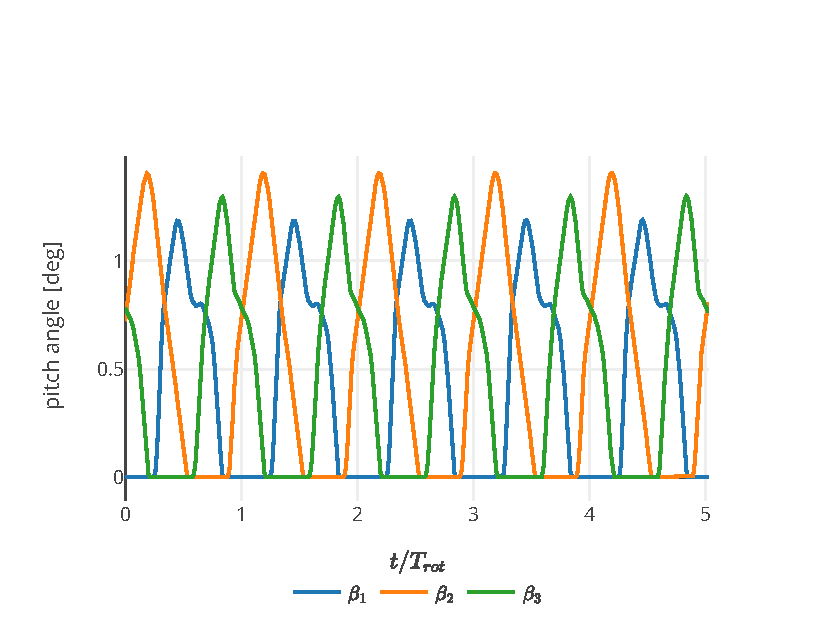
\includegraphics[width=\textwidth]{images/pitch_angle_rollout_10_7ms.pdf}
      \caption{WINDL pitch activity at 10.7 m/s (rated speed)}
      \label{fig:pitch-at-rated}
      % run 7
  \end{subfigure}
  \begin{subfigure}[b]{0.48\textwidth}
      \centering
      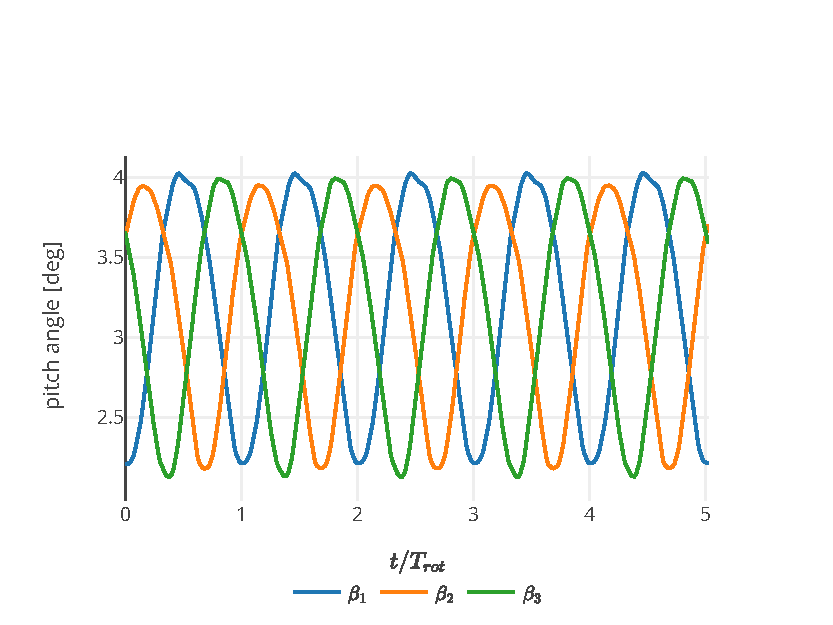
\includegraphics[width=\textwidth]{images/pitch_angle_rollout_11_5ms.pdf}
      \caption{WINDL pitch activity at 11.5 m/s}
      \label{fig:pitch-above-rated}
      % run 15
  \end{subfigure}
  \caption{WINDL pitch activity at rated and slightly above rated speed. While above rated speed, the pitching motion is sinusodial, it is capped and asymmetric at rated speed.}
  \label{fig:pitch-around-rated}
  % sac-steady-final, data_0, reeval_468
\end{figure}

Figure \ref{fig:pitch-around-rated} shows the different pitch behavior of \ac{WINDL} at and above rated speed. Slightly above rated speed, a symmetrical sinusoidal motion is applied to all blades similar to Figure \ref{fig:steady-rollout-pitch}. At rated speed, this motion is cut off at 0 degrees. In Subfigure \ref{fig:pitch-at-rated}, a phenomenon can be observed where the different blades are actuated visibly differently. Blade number two performs a high-magnitude and close to sinusoidal motion, while blade one and three are actuated with a lower magnitude. The bDEL values for the individual blades at 10.7 m/s are $[1.88\text{M}, 1.51\text{M}, 1.73\text{M}]$. There is no explicit incentive to actuate evenly across all blades, but for higher wind speeds like in Subfigure \ref{fig:pitch-above-rated} the policy intrinsically keeps their motions similar. Note that even in this plot, there is a slight difference in actuation rate. We hypothesize the uneven behavior at rated speed to be optimal or at least not penalized in the reward function. Keeping a full sinusoidal motion for every blade is impossible due to the low base pitch angle. To keep one blade as close to a sinusoidal motion as possible (blade 2 in this case) and to use the other two to keep up the thrust might improve the total reward more than having all three incur equally bad loads. We briefly investigated a reward penalty for differing behavior of the individual blades but found this to not solve the problem.

\subsection{Discussion}

We show WINDL to produce significantly lower bDELs in the transition period from 10 to 12 m/s, offsetting the current state-of-the-art by 42.9\%. This comes at the expense of a decrease in power of 0.62\%. We see a peak in loads at rated speed, which is consistent with expectations for all policies. Using a load-minimizing policy that can work at rated speed brings high load saving potential. While above rated, WINDL does not exhibit a decrease in power, some power yield is lost in the transition period. For most wind turbine models, such a significant impact on the total energy yield of the wind turbine likely offsets the benefit of lower blade loads by a wide margin. To judge whether the decrease in power is justified by the load reduction, an extensive analysis is required, taking into account material properties, electricity sale prices, and the weather on site. The result of this analysis would be a wind speed threshold, below which it is not feasible to operate WINDL anymore and where it should be ramped down. Technically, it could be operated all the way down to set-in speed, but we only expect an application below rated wind speed to be sensible in very few situations.

Furthermore, we observe a phenomenon around rated speed, where WINDL exhibits unequal pitching action. Our current reward function might incentivize this behavior and we found no trivial way to disincentivize it. It could even be globally optimal to do so, as the higher load on the two other blades might be overcompensated by the lower load on blade number two. To evenly distribute wear, a fix could involve rotating the pitch action mappings to the blades, so each blade gets to be number two at some point. Future work could try to investigate this phenomenon or find a better fix.

\section{Naive Performance Turbulent Wind}
\label{section:results-naive-turbulent}

\begin{summary}
In this section, we train WINDL in the turbulent wind using the same hyperparameters as used for the steady wind. We find that this results in slightly better blade wear but brings a disproportionate hit to pitch wear and power yield. We conclude that different hyperparameters are needed for different wind scenarios.
\end{summary}

For this section, we train a model with four different random seeds in the turbulent wind scenario to 1000 epochs (16M environment interactions) and choose the best performing checkpoint with respect to bDEL. We use the same hyperparameters as in the steady wind, see Table \ref{table:hyperparameters}. For our evaluation, we measure performance on all wind speeds between 10 and 20 m/s across eight random seeds and with a resolution of 0.1 m/s steps.

Depending on the location of a turbine, it will not only experience steady wind during operation. Thunderstorms, strong thermal convection, or other phenomena can cause the wind to rapidly change speed and direction. Such a rapid change can cause structural damage through high loads on a wind turbine, if the load minimizing control policy is not able to counteract in time. While in the steady wind, the major trade-off concerns only blade and pitch wear, in the turbulent wind there is a three-way trade-off between power yield, blade wear, and pitch wear. A good control policy pitches aggressively at the start of strong gusts to reduce blade wear and pitches conservatively in low winds to maximize energy yield. It optimizes power yield, blade fatigue loads, blade extreme loads, and pitch fatigue loads simultaneously. Optimally, WINDL can learn this with the same hyperparameters that yielded good results in the steady wind scenario showing hyperparameter insensitivity.

\subsection{Presentation}

\begin{figure}[hbt!]
  \centering
  \begin{subfigure}[b]{0.48\textwidth}
      \centering
      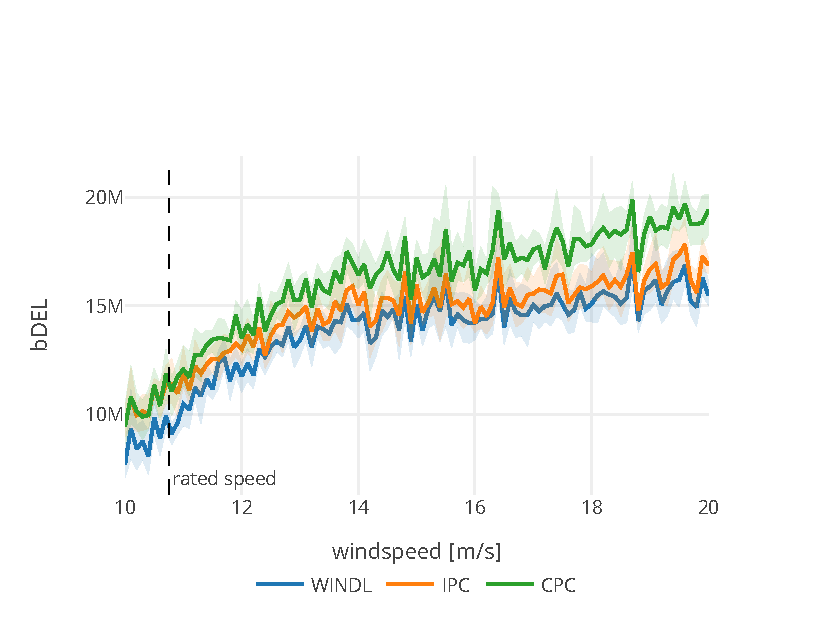
\includegraphics[width=\textwidth]{images/naive_sweep_bdel.pdf}
      \caption{blade-DELs against windspeed}
      \label{fig:naive-sweep-bdel}
  \end{subfigure}
  \begin{subfigure}[b]{0.48\textwidth}
      \centering
      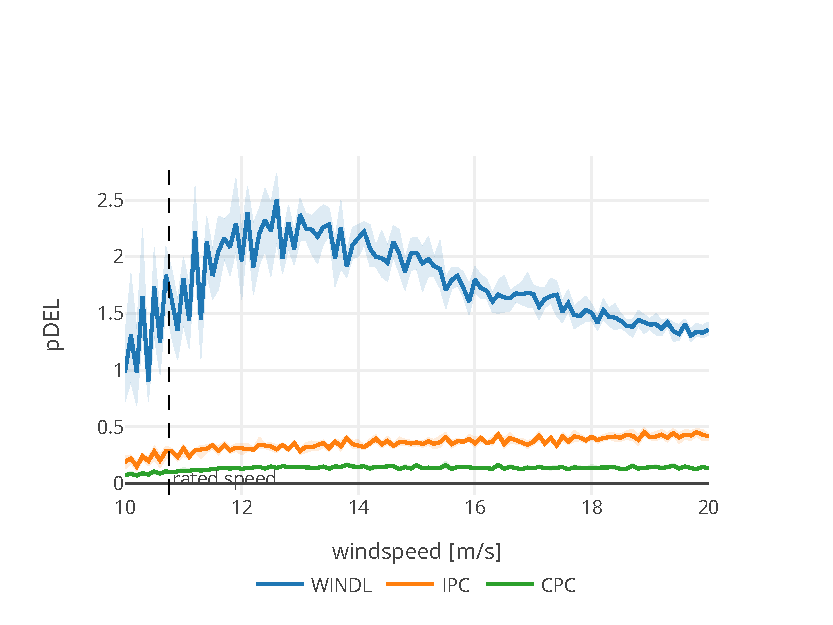
\includegraphics[width=\textwidth]{images/naive_sweep_pdel.pdf}
      \caption{pitch-DELs against windspeed}
      \label{fig:naive-sweep-pdel}
  \end{subfigure}
  \begin{subfigure}[b]{0.48\textwidth}
    \centering
    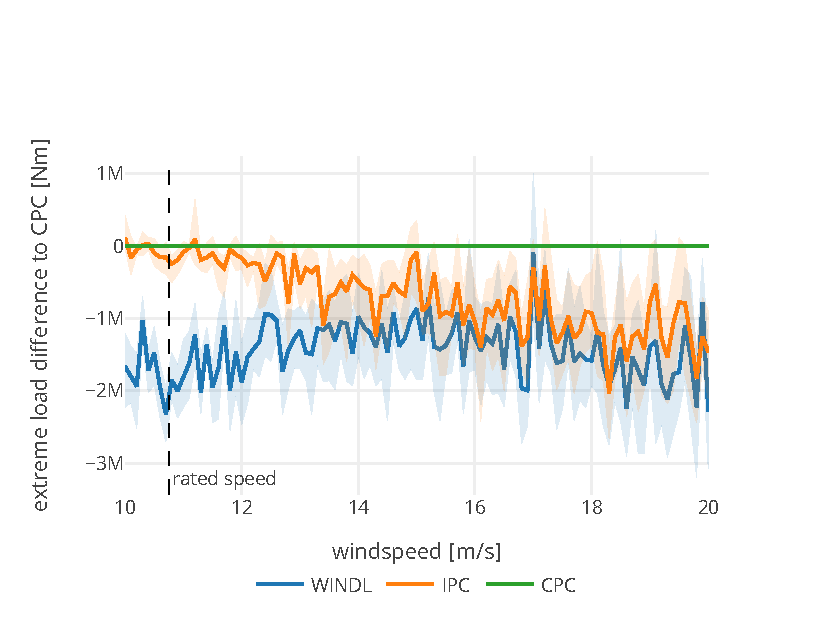
\includegraphics[width=\textwidth]{images/naive_sweep_extreme.pdf}
    \caption{Relative extreme loads compared to CPC performance against windspeed}
    \label{fig:naive-sweep-extreme}
\end{subfigure}
\begin{subfigure}[b]{0.48\textwidth}
    \centering
    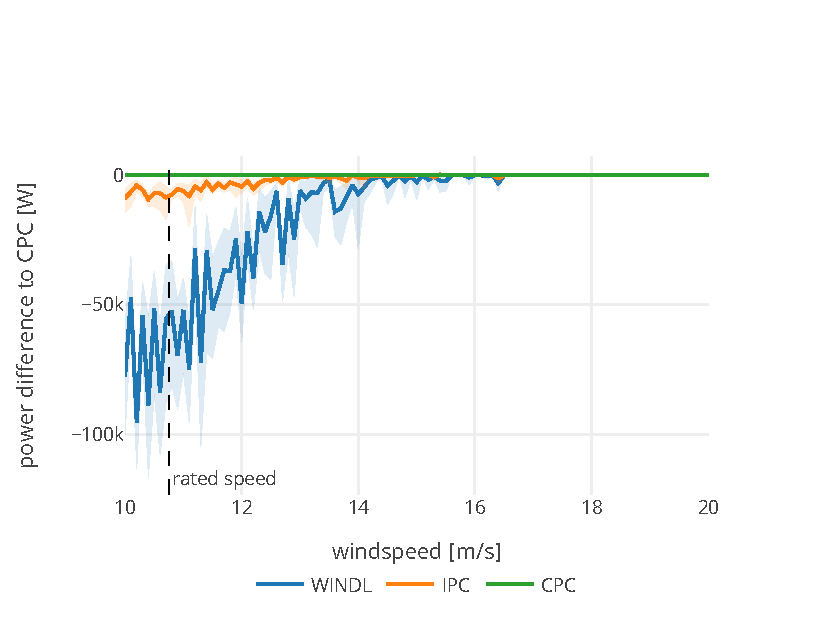
\includegraphics[width=\textwidth]{images/naive_sweep_power.pdf}
    \caption{Relative power production compared to CPC performance against windspeed}
    \label{fig:naive-sweep-power}
\end{subfigure}
  \caption{The transfer performance of a model trained in the turbulent wind scenario with hyperparameters from the steady wind, compared to IPC and CPC performance. Lower is better except for power production.}
  \label{fig:naive-sweep}
  % sac-fullturb-5, data_12, reeval_225
\end{figure}

\begin{table}[hbt!]
  \centering
  \begin{tabular}{c@{\hskip 0.7cm}cc@{\hskip 0.7cm}cc}
    \toprule
    & \multicolumn{2}{c}{WINDL to IPC} & \multicolumn{2}{c}{WINDL to CPC} \\
    Metric & 10-12 m/s & 12-20 m/s & 10-12 m/s & 12-20 m/s \\
    \midrule
    bDEL & -1.26M (11.19\%) & -0.74M (4.61\%) & -1.69M (13.94\%) & -2.47M (14.11\%) \\
    pDEL & +1.40 (-532\%) & +1.41 (-403\%) & +1.56 (-1402\%) & +1.64 (-1180\%) \\
    extreme [Nm] & -1.60M (4.62\%) & -0.55M (1.85\%) & -1.71M (4.91\%) & -1.37M (4.78\%) \\
    power [W] & -50.3K (-0.58\%) & -3.80K (-0.04\%) & -56K (-0.65\%) & -4.27K (-0.04\%) \\
    \bottomrule
  \end{tabular}
  % sac-fullturb-4, data_12, reeval_225
  \caption{Mean absolute difference and mean relative improvement of naive WINDL as shown in Figure \ref{fig:naive-sweep} compared to the IPC and the CPC, split in around-rated (10-12 m/s) and above-rated (12-20 m/s).}
  \label{table:naive-improvements}
\end{table}

Figure \ref{fig:naive-sweep} shows the performance of a WINDL policy that was chosen among four trainings to 1000 epochs by picking maximal bDEL performance. Four different metrics are evaluated for different wind speeds in the range of 10 to 20 m/s across eight turbulent seeds per wind speed with a wind speed resolution of 0.1 m/s. Subplot \ref{fig:naive-sweep-bdel} and Subplot \ref{fig:naive-sweep-pdel} plot absolute values, while Subplot \ref{fig:naive-sweep-extreme} and Subplot \ref{fig:naive-sweep-power} plot relative values to CPC performance to improve readability of the plots. The averaged absolute differences to the baselines, and in brackets the averaged relative improvements of these performances, are shown in Table \ref{table:naive-improvements}. Note that for bDEL, pDEL and extreme loads, less is better, while for power, more is better.

WINDL exhibits lower blade fatigue loads than the IPC baseline by 4.61\% above rated and 11.19\% around rated (Subplot \ref{fig:naive-sweep-bdel}). An improvement can be seen across the entire range of wind speeds, but most prominently up to 14 m/s. Also, WINDL exhibits lower extreme loads as visible in Subplot \ref{fig:naive-sweep-extreme}. Between 10 and 12 m/s, extreme loads are 4.65\% lower than the IPC baseline and 4.95\% lower than the CPC, while above rated between 12 and 20 m/s, they are 1.91\% lower than the IPC and 4.68\% lower than the CPC. This comes at the price of significantly higher pitch DELs by 376\% compared to the IPC and 1157\% compared to the CPC (Subplot \ref{fig:naive-sweep-pdel}). Also, WINDL exhibits power losses of 3.8 kW compared to the IPC above rated and 50 kw below rated (Subplot \ref{fig:naive-sweep-power}). The power loss is only significantly visible below 14 m/s and not visible anymore above 16.5 m/s.  Because above 16.5 m/s wind speed, most turbulences in the \ac{NTM} do not reach speeds below rated, the generator stays at saturation levels the entire time.

Compared to the policy performance in Figure \ref{fig:transfer-turbulent}, the blade DELs are better. The pitch wear exhibited by the policy trained in the turbulent wind is worse than the policy trained in the steady wind but evaluated in turbulent. In contrast to the steady wind in Figure \ref{fig:transition}, blade and pitch wear do not peak at rated speed for any of the control policies. The absence of this peak is caused by the magnitude of wear induced through turbulence, which overshadows wear induced by control policies. When compared to the steady wind above rated performance in Figure \ref{fig:steady-sweep}, both blade and pitch wear values are higher by ca. one order of magnitude. As such, wear effects induced by the steady wind shear and control policies are overshadowed by the wear induced through turbulences.

\subsection{Discussion}

WINDL outperforms the IPC with respect to blade DELs by 4.6\% above rated. 

Besides reducing blade fatigue loads in the DEL metric, WINDL does also reduce extreme loads below IPC levels. There is an incentive to do so, because the reward function will react negatively to extreme loads. As extreme loads are relatively short events, the high-pass filter for the $\tilde c_s$ component will not filter them out, and they will increase the blade penalty. Especially at rated speed where extreme loads are high, this significant decrease can prevent fatal damage to blades in gusts. Furthermore, blades can be designed with a lower breaking point, which will reduce construction costs.

Section \ref{section:results-steady-fatigue} has shown WINDL to be capable of finding a high performing policy for the steady wind scenario with regards to both optimization aims from the steady wind: pitch wear and blade wear. While in the steady wind, it is not explicitly incentivized to keep pitch activity low, the smoothness regularization automatically does so. In the turbulent scenario, this is not the case. The agent trained on the turbulent wind learns to pitch more aggressively than an agent trained on the steady wind, which shows that the agent exploits the pitch blade trade-off to optimize blade bendings only. This exploitation is a major argument against WINDL adoption, and pitch wear of that magnitude is likely not acceptable even for turbines with sturdy pitch bearings. 

The exploitation does also apply to power production, and as soon as WINDL has the option to trade it for blade bending, it does so. Power production is not captured at all by our reward function. While the assistive CPC has the aim to maximize power, the reinforcement learned load control policy manages to interfere with this policy.

Concludingly, WINDL does successfully optimize the primary optimization goal blade wear below IPC levels. However, the naive policy is not well suited as a drop-in replacement for IPC controllers, because it disregards secondary optimization aims. While in the steady wind, an explicit penalty for pitch wear is not necessary, the turbulent wind scenario requires a hyperparameter modification to regard secondary optimization aims.

\section{Adjusted For Pitch Loads}
\label{section:results-adjusted}

\begin{summary}
In this section, we train WINDL with an adjusted hyperparameter set in the turbulent wind. We find that the adjusted WINDL produces significantly lower blade loads than current baseline controllers, potentially setting a new state-of-the-art for wind turbine load control. However, we observe drawbacks through more pitch wear and some power loss. We investigate two example rollouts to observe the strategies that WINDL learned and find that it can choose when to utilize pitch actions smartly and that it pitches through low-wind scenarios to alleviate extreme loads.
\end{summary}

To train the model for this section, we utilize adjusted hyperparameters for the turbulent wind, as outlined in the rightmost column of Table \ref{table:hyperparameters}. These hyperparameters were obtained by tuning for both blade and pitch wear. We train four random seeds up to 1500 epochs, which corresponds to 36M environment interactions, and pick the best performing checkpoint with respect to bDEL for evaluation.

Reinforcement learning algorithms are benchmarked on a variety of tasks and shall perform well on all of them without changes to hyperparameters. In our case, we can tune the hyperparameters to the specific task at hand to reach maximal performance. For a production use of WINDL, one hyperparameter set for all wind scenarios would be desirable, but for a proof of concept, different sets can show the potential performance gains. 

To obtain these results, we perform a hyperparameter search with the aim of finding the best set of hyperparameters for the turbulent wind. Best referrs mainly to final policy performance, with training stability and convergence speed as secondary aims. The new set of hyperparameters is presented in Table \ref{table:hyperparameters} in the column \textit{turbulent wind}. Smoothing parameters were increased to $\lambdatemp=0.2, \lambdaspat=0.2$, but in contrast to the steady wind, purely smoothness regularized pitch control exhibited too high pitch activity. The pitch performance did not differ much from naive performance as shown in Section \ref{section:results-naive-turbulent}. Adding the pitch penalty $\rcolemanact=0.02$ into the reward function improved pitch handling, but significantly destabilized training. Decreasing the learning rates by factor 3, increasing the discounting factor to $\gamma=0.99$, and increasing the number of environment interactions per epoch by 50\% alleviated these issues. Lastly, slightly increasing IPC control play to $\ipcplay=\pm4$ and allowing $c_S$ action control drastically improved blade wear with just a marginal hit to pitch activity.

\subsection{Presentation}

\begin{figure}[hbt!]
  \centering
  \begin{subfigure}[b]{0.48\textwidth}
      \centering
      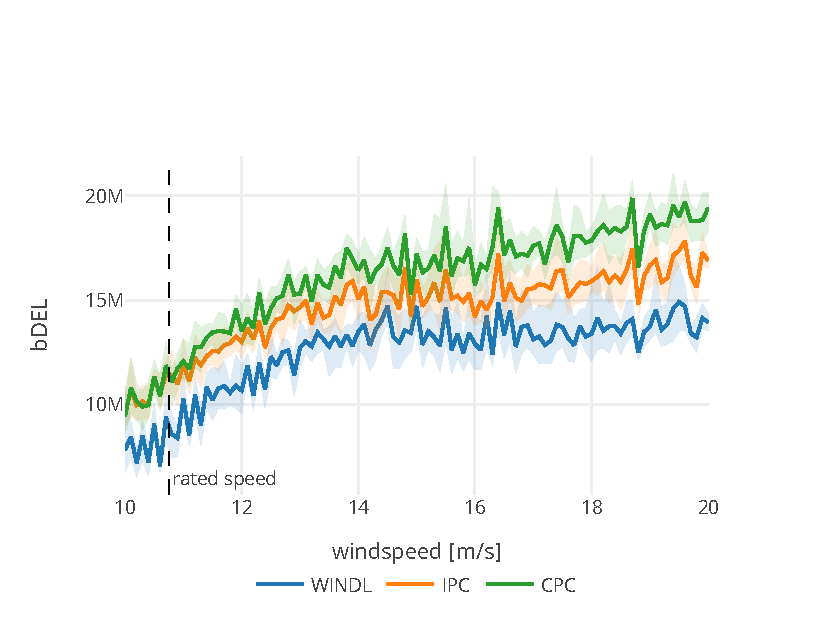
\includegraphics[width=\textwidth]{images/adjusted_bdelopt_bdel.pdf}
      \caption{blade-DELs against windspeed}
      \label{fig:adjusted-bdelopt-bdel}
  \end{subfigure}
  \begin{subfigure}[b]{0.48\textwidth}
      \centering
      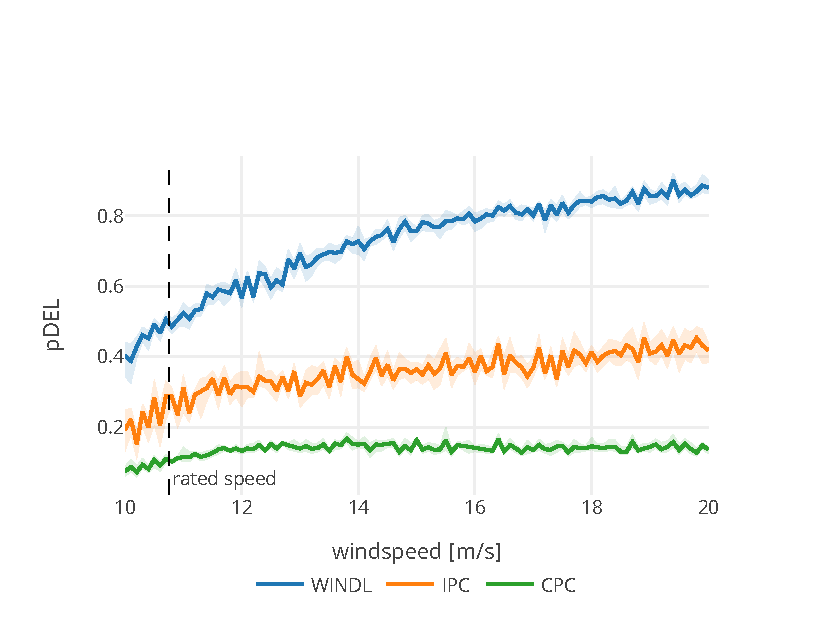
\includegraphics[width=\textwidth]{images/adjusted_bdelopt_pdel.pdf}
      \caption{pitch-DELs against windspeed}
      \label{fig:adjusted-bdelopt-pdel}
  \end{subfigure}
  \begin{subfigure}[b]{0.48\textwidth}
    \centering
    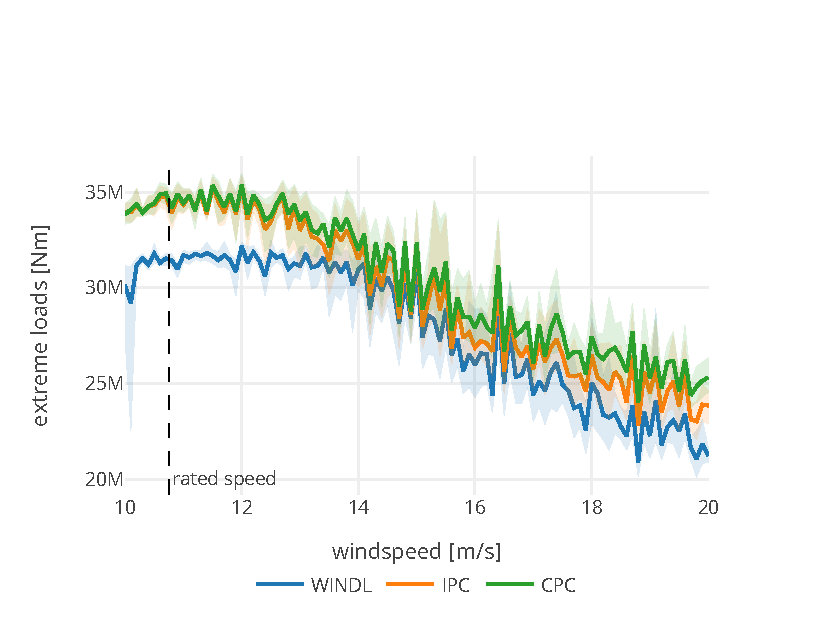
\includegraphics[width=\textwidth]{images/adjusted_bdelopt_extreme.pdf}
    \caption{Extreme loads against windspeed}
    \label{fig:adjusted-bdelopt-extreme}
  \end{subfigure}
  \begin{subfigure}[b]{0.48\textwidth}
      \centering
      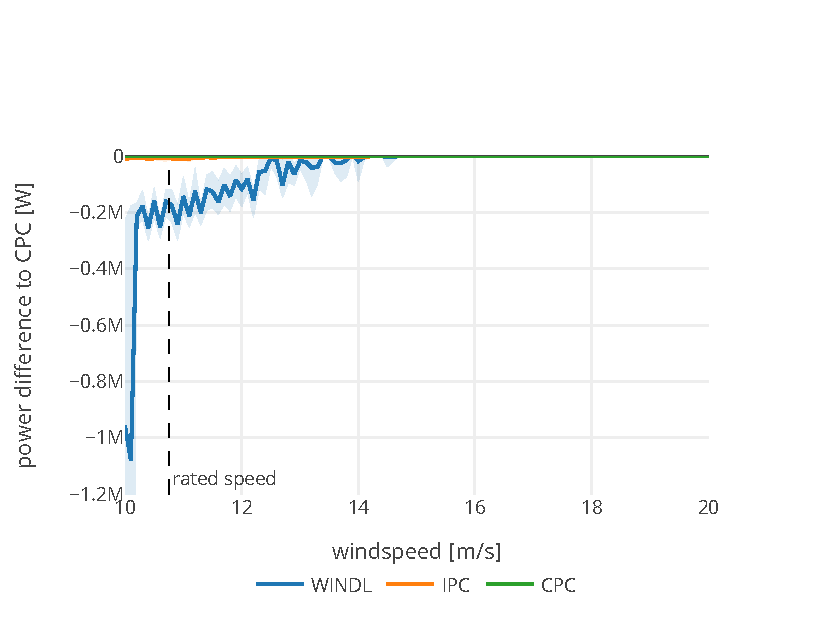
\includegraphics[width=\textwidth]{images/adjusted_bdelopt_power.pdf}
      \caption{Relative power production compared to CPC performance against windspeed}
      \label{fig:adjusted-bdelopt-power}
  \end{subfigure}
  \caption{The performance of adjusted WINDL, compared to IPC and CPC performance. Lower is better except for power production.}
  \label{fig:adjusted-bdelopt}
  % sac-turb-optim-1, data_42, turb_reeval_1430
\end{figure}

\begin{table}[hbt!]
  \centering
  \begin{tabular}{c@{\hskip 0.7cm}cc@{\hskip 0.7cm}cc}
    \toprule
    & \multicolumn{2}{c}{WINDL to IPC} & \multicolumn{2}{c}{WINDL to CPC} \\
    Metric & 10-12 m/s & 12-20 m/s & 10-12 m/s & 12-20 m/s \\
    \midrule
    bDEL & -2.27M (19.8\%) & -2.11M (13.45\%) & -2.69M (22.28\%) & -3.85M (22.04\%) \\
    pDEL & +0.24 (-111\%) & +0.4 (-110\%) & +0.4 (-386\%) & +0.63 (-455\%) \\
    extreme [Nm] & -3.07M (8.86\%) & -1.56M (5.45\%) & -3.17M (9.14\%) & -2.39M (8.27\%) \\
    power [W] & -241K (-2.83\%) & -9.38K (-0.1\%) & -247K (-2.89\%) & -9.77K (-0.1\%) \\
    \bottomrule
  \end{tabular}
  % sac-turb-optim-1, data_42, turb_reeval_1430
  \caption{Mean absolute difference and mean relative improvement of adjusted WINDL compared to the IPC and the CPC, split in around-rated (10-12 m/s) and above-rated (12-20 m/s).}
  \label{table:improvements-bdelopt}
\end{table}

Figure \ref{fig:adjusted-bdelopt} and Table \ref{table:improvements-bdelopt} show the final policy performance of a policy trained with the adjusted hyperparameters for the turbulent wind. The performance of the WINDL, IPC and CPC policy is evaluated in eight different turbulent seeds for all wind speeds from 10 - 20 m/s with a resolution of 0.1 m/s. All subplots in Figure \ref{fig:adjusted-bdelopt} show absolute values except for Subplot \ref{fig:adjusted-bdelopt-power}, which shows relative values compared to the CPC policy to improve readability.

Across the entire wind span, a significant reduction in bDELs compared to the difference between IPC and CPC is visible (Subplot \ref{fig:adjusted-bdelopt-bdel}). The first row in Table \ref{table:improvements-bdelopt} quantifies this to 13\% lower blade wear above rated compared to the current state-of-the-art. Especially around rated speed, where the IPC does not improve upon the CPC a lot, WINDL still delivers a significant fatigue load reduction. 

This comes at the price of higher blade DELs as visible in Subplot \ref{fig:adjusted-bdelopt-pdel}. Pitch actuation rises with wind speed and relative wear levels are consistent to approximately double the IPC rates across the entire operating range (row 2, Table \ref{table:improvements-bdelopt}). 

The IPC is deactivated in around- and below-rated wind speeds to prevent power loss, which results in only a 0.015\% decrease from CPC to IPC. WINDL exhibits one order of magnitude higher power losses above rated (-0.1\%) and two orders of magnitude higher around rated speed (-2.89\%) compared to the CPC, which generates the maximum amount of power (see row 4, Table \ref{table:improvements-bdelopt}). As visible in Subplot \ref{fig:adjusted-bdelopt-power}, this loss happens mostly below 14 m/s, and above 16 m/s no more power losses are measurable. Congruent to previous policies, this is consistent with the turbulence model, which will not dip below rated speed for mean wind speeds above 16 m/s.

Together with the loss in power, the reduction of extreme loads is most prominent below 14 m/s (see Subplot \ref{fig:adjusted-bdelopt-extreme}). Around rated, an extreme load reduction of 8.86\% compared to the IPC policy is achieved (see row 3 Table \ref{table:improvements-bdelopt}). This extreme load reduction coincides with the power loss and might be due to WINDL exploiting a trade-off. Around rated, extreme values are maximal and an extreme load reduction is most desired. The highest extreme load across all seeds is reduced from 3.9M Nm for the IPC to 3.5M Nm for WINDL with mean values well below that (see lower wind speeds in Subplot \ref{fig:adjusted-bdelopt-extreme}). Above rated, an improvement of 5.45\% compared to the IPC is visible. Some of this improvement is to be credited to the loss in power, which allows for an extreme load saving policy around rated speed. Taking into account only the region from 14 m/s to 20 m/s where WINDL does not lose much power, the improvement drops to 5.3\%.

Compared to the naive policy as presented in Section \ref{section:results-naive-turbulent}, the hyperparameter adjustments have brought a significant improvement in all quantities subject to optimization except for power. When directly comparing Table \ref{table:improvements-bdelopt} to Table \ref{table:naive-improvements}, the adjusted WINDL achieves significantly lower blade bendings, pitch bendings, and extreme load than the naive version.

\subsection{Investigating Policy Actions}

In this subsection, we pick two example rollouts in different wind scenarios to clarify the difference between the WINDL and IPC policy. We demonstrate how WINDL gains upon the IPC and investigate the power loss phenomenon.

\begin{figure}[hbt]
  \centering
  \begin{subfigure}[b]{0.48\textwidth}
      \centering
      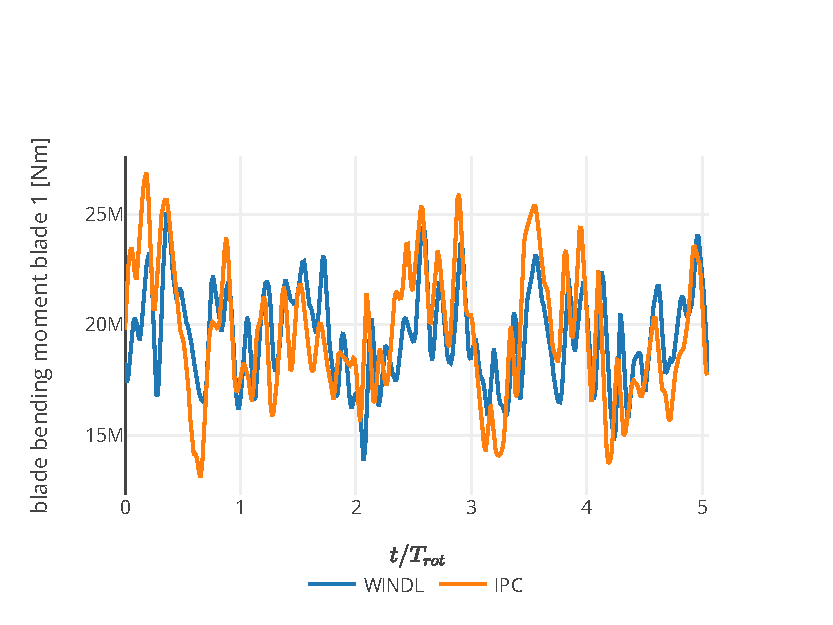
\includegraphics[width=\textwidth]{images/adjusted_blade_rollout.pdf}
      \caption{Blade bendings over time for mean wind speed 14 m/s}
      \label{fig:adjusted-rollout-blade}
  \end{subfigure}
  \begin{subfigure}[b]{0.48\textwidth}
    \centering
    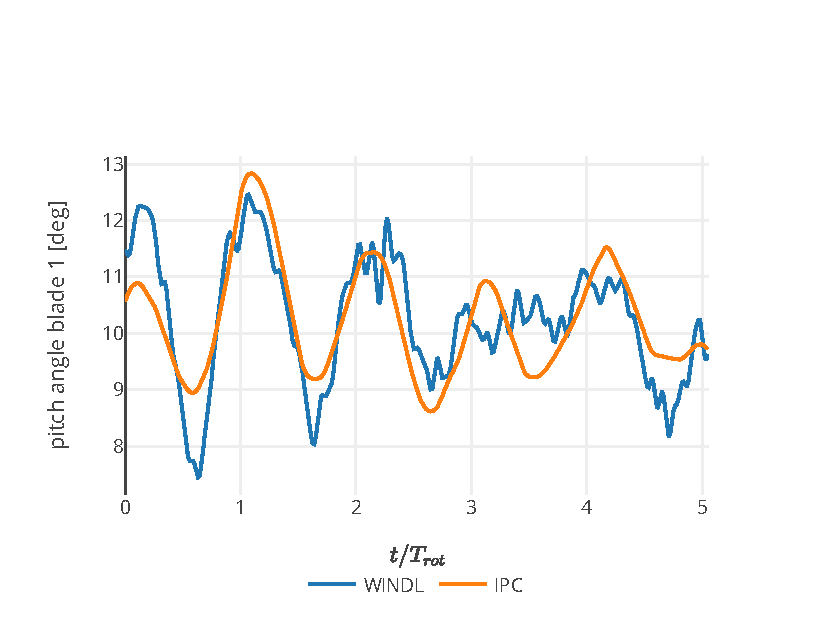
\includegraphics[width=\textwidth]{images/adjusted_pitch_rollout.pdf}
    \caption{Pitch actions over time for mean wind speed 14 m/s}
    \label{fig:adjusted-rollout-pitch}
  \end{subfigure}
  \begin{subfigure}[b]{0.48\textwidth}
      \centering
      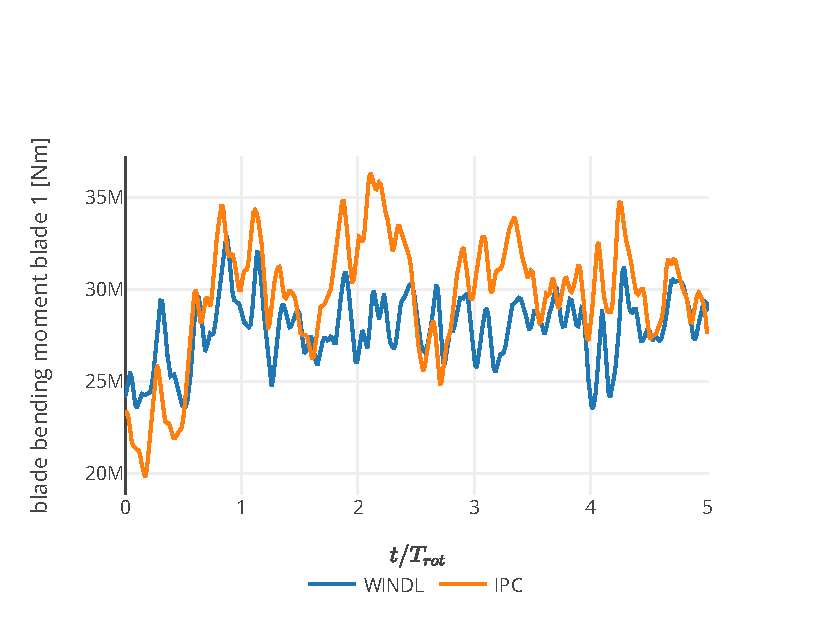
\includegraphics[width=\textwidth]{images/adjusted_lowwind_blade_rollout.pdf}
      \caption{Blade bendings over time for mean wind speed 12 m/s}
      \label{fig:adjusted-rollout-lowwind-blade}
  \end{subfigure}
  \begin{subfigure}[b]{0.48\textwidth}
    \centering
    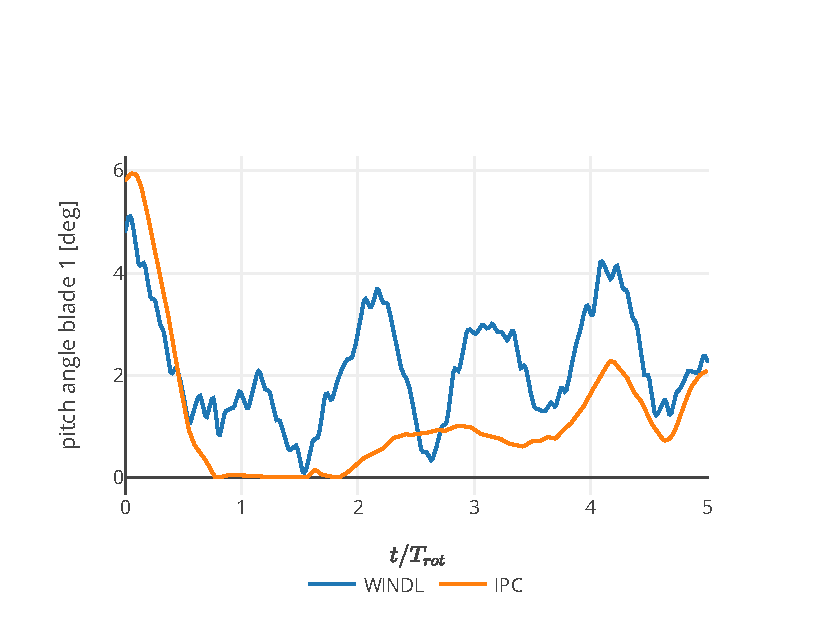
\includegraphics[width=\textwidth]{images/adjusted_lowwind_pitch_rollout.pdf}
    \caption{Pitch actions over time for mean wind speed 12 m/s}
    \label{fig:adjusted-rollout-lowwind-pitch}
  \end{subfigure}
  \caption{Rollouts of the pitch actions and blade bendings for the first blade in two different turbulent wind scenarios, one with mean wind speed 14 m/s and one with 12 m/s. The two other blades are ommitted for clarity.}
  \label{fig:adjusted-rollout}
  % sac-turb-optim-1, data_42, turb_reeval_1430, eval_run 160 (12m/s) and 320 (14m/s)
\end{figure}

Figure \ref{fig:adjusted-rollout} shows two rollouts of pitch actions and the corresponding blade movements of WINDL and the IPC for the same wind scenario. Only the actions of blade one are shown for brevity, as the other two blades behave similarly with a phase offset of 120 degrees. The time axis is plotted in multiples of the rotation time ($t/T_{rot}$). Five rotations are shown, which corresponds to 4.5 seconds of simulation time at rated rotor speed. In the blade bending plots, low amplitudes between high and low bending moments are desired for fatigue load reduction and low maxima are desired for extreme load reduction.

In Subplot \ref{fig:adjusted-rollout-pitch}, the difference of pitch actions between WINDL and the IPC is clearly visible. Similar to the steady wind, WINDL pitches on both low and high frequencies, while the IPC only utilizes a single low frequency. When not necessary, WINDL deactivates the low-frequency pitch activity almost completely as visible between rotation 3 and 4. The corresponding blade bendings in the same time on Subplot \ref{fig:adjusted-rollout-blade} show that this corresponds with a lower bending amplitude, suggesting that some of the IPC loads are induced by the supposedly load minimizing pitching policy. At other times like between rotation 0 and 1, WINDL pitches significantly more aggressively than the IPC, which also results in a bending amplitude reduction. The IPC reactions are strongly lowpass-filtered to improve IPC stability, and consequently it is not able to adjust its actions as dynamically as WINDL does. WINDL shows that is is beneficial to allow nuances in the incoming wind to decide over the amplitude of pitching action.

Subplot \ref{fig:adjusted-rollout-lowwind-pitch} shows a wind scenario where a turbulence dips the mean incoming wind speed below rated speed. The mean wind speed for this scenario is 12 m/s, but through a turbulence, it is reduced past 10.75 m/s for a short period of time. This is the period of time where WINDL has the most significant extreme load reduction. As visible in Subplot \ref{fig:adjusted-rollout-lowwind-blade}, the IPC experiences an extreme load at rotation 2 while WINDL does not. This is due to the different pitching actions as shown in Subplot \ref{fig:adjusted-rollout-lowwind-pitch}. The IPC policy is ramped down to no activity to conserve power, but WINDL pitches quite aggressively, especially around the extreme load at rotation 2. This comes with a loss in power. While in Subplot \ref{fig:adjusted-rollout-pitch}, both policies produce the same amount of power at 10 MW, WINDL has an average power level of 8.96 MW, and the IPC of 9.29 MW across the time shown in Subplot \ref{fig:adjusted-rollout-lowwind-pitch}. 

\begin{figure}
  \centering
  \begin{subfigure}[b]{0.48\textwidth}
      \centering
      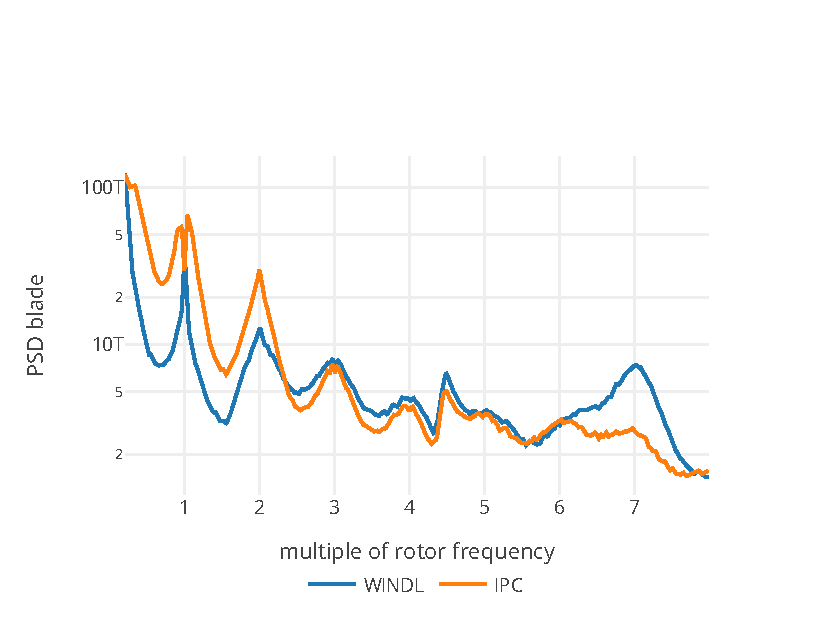
\includegraphics[width=\textwidth]{images/turbulent_psd_blade.pdf}
      \caption{Average blade bending PSD above rated}
      \label{fig:adjusted-psd-blade}
  \end{subfigure}
  \begin{subfigure}[b]{0.48\textwidth}
    \centering
    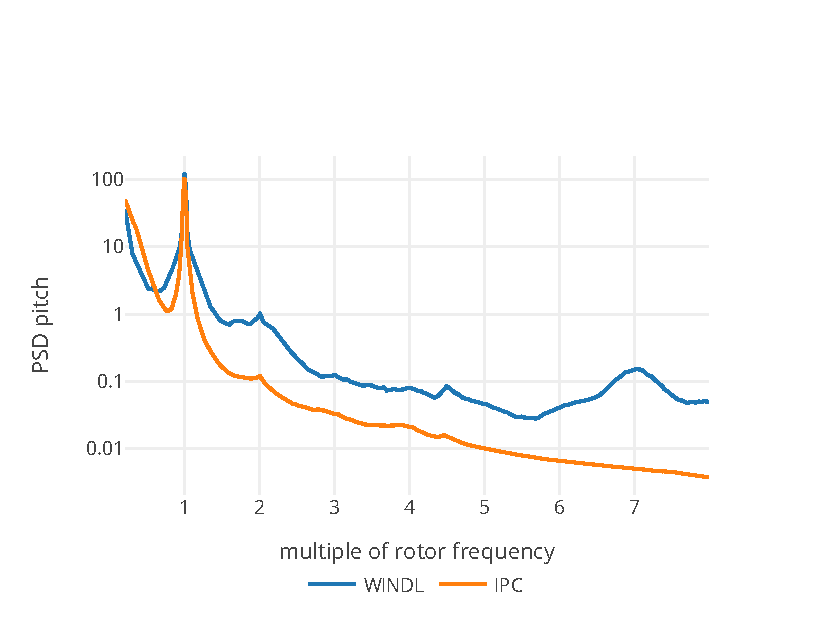
\includegraphics[width=\textwidth]{images/turbulent_psd_pitch.pdf}
    \caption{Average pitch actuation PSD above rated}
    \label{fig:adjusted-psd-pitch}
  \end{subfigure}
  \caption{PSD plots of the pitch actuation and blade bendings, averaged across 648 rollouts above rated and across all three blades. Lower is better.}
  \label{fig:adjusted-psd}
  % sac-turb-optim-1, data_42, turb_reeval_1430, group 2160:
\end{figure}

For further investigation, we plot the \ac{PSD} for both pitch actuation and blade bending averaged across 648 rollouts above rated speed and across all three blades in Figure \ref{fig:adjusted-psd}. This averaging smoothes out turbulence effects and extracts the impact of the policies. Subplot \ref{fig:adjusted-psd-pitch} shows the pitch actuation across the frequency band. The IPC has a sharp spike at the 1p frequency and not much more frequency contents. This is congruent to the behavior below rated speed as shown in Figure \ref{fig:steady-rollout-pitch-psd}. WINDL also exhibits the peak at 1p with a slightly higher maximum value, but with a flatter curvature than the IPC. Actuation around the 1p frequency of the IPC is minimal, while WINDL performs some work between 0.7 and 1.3p. This shows very clearly in the blade PSD in Subplot \ref{fig:adjusted-psd-blade}. Around the 1p frequency, the IPC exhibits two peaks, which are likely the main cause of blade DELs for the IPC. WINDL does not have these peaks around 1p. Also at 2p, WINDL exhibits more pitching action than the IPC and incurs less blade loads. For some reason, WINDL learned to also pitch on the 7p frequency, which seems to be detrimental to blade loads on that side. Such high frequency noise could easily be masked by the noise of the turbulence, and learning the system behavior on that frequency likely poses a challenge, leading WINDL into misbehavior. In contrast to the behavior in the steady wind from Figure \ref{fig:steady-rollout-pitch-psd}, WINDL does not have peaks at 3p, 4p, 5p, and 6p but a continuously lifted pitch band in comparison to the IPC. This is likely the source of the higher pitch loads, together with the slightly higher actuation at 1p. 

\subsection{Discussion}

The IPC idea first presented by \citet{bossanyiIndividualBladePitch2003} introduced a funtamentally different idea than the previous state-of-the-art, the CPC, reducing blade fatigue loads significantly at the cost of some pitch wear. It slowly gains adoption, as the trade-off pays off on some turbines. WINDL shows to be capable of advancing this trade-off even further. With hyperparameters adjusted to the challenges of the turbulent wind, it outperforms the state-of-the-art IPC policy with respect to blade fatigue loads by a similar margin as the IPC outperforms the CPC. Congruent with the switch from CPC to IPC, this does happen at the expense of pitch activity. Furthermore, WINDL shows a reduction of extreme loads, which is partially achieved by trading power production but partially also due to intelligent pitching behavior. 

WINDL outperforms the IPC above rated by 13.5\% lower fatigue loads at the expense of 110\% higher pitch wear. The reduction is comparable to the improvement of switching from a CPC to an IPC, which brings 9.87\% lower blade DELs at the expense of 67.8\% higher pitch wear. Furthermore, WINDL shows a reduction of extreme loads of 5.45\% above rated compared to the IPC, which comes with a loss of power of 0.1\%.

In the turbulent wind setting, WINDL again showed the potential to black-box optimize to a performance level which matches or outperforms model-informed baselines. This requires multiple adjustments of hyperparameters to adjust WINDL to the wind scenario at hand. The need for such hyperparameter adjustments is a set-back to the idea of reinforcement learning to black-box optimize any scenario to perfection and a hindrance to adoptment, as the wind scenarios a turbine will operate in are only partially predictable.

Extreme load reductions are especially relevant around rated speed. WINDL trades some power for lower extreme loads. Whether this is economically feasible is dependent on the turbine model and the possible blade price reduction that goes with it. If this extreme load reduction is not wanted, future work could implement a policy ramp down around rated speed similar to the IPC to prevent power loss. Such a ramp down would increase blade wear and extreme loads but conserve power and pitch wear around rated speed. Future work could also investigate a power penalty in the reward function.

The high performance stems from the ability of WINDL to adapt its behavior to the turbulence at hand based on more information than purely average wind speed or the current blade loads. Through the extraction of knowledge from the entire sensor array and the near past, it decides when to invest pitching actions and when to conserve them. Furthermore, it alleviates extreme loads during temporal wind speed dips below rated by retaining a pitching motion where the IPC ramps down any pitching behavior. Pitch actuation around the 1p frequency and on the 2p frequency lead to a reduction in blade loads on these frequencies, giving WINDL an edge over the IPC in terms of blade wear.


\section{Tuning For The Pitch-blade Trade-off}
\label{section:results-pb-trade-off}

\begin{summary}
In this section, we investigate one of the trade-offs in controller design, the trade between pitch and blade loads. We try different hyperparameter combinations and show that through adjustment of training hyperparameters, the optimization focus can be shifted between the trade-off goals. Counterintuitively, the policy performance is not controlled mainly through the reward function coefficients but through other hyperparameters.
\end{summary}

For this section, we train each hyperparameter combination four times with different seeds up to 500 epochs (approx. 7M environment interactions) in the steady wind scenario or 1500 epochs (approx 40M environment interactions) in the turbulent wind scenario. 

Depending on the wind turbine model, materials, and resource costs, the blades or the pitch system can take a more significant part of the total costs. For smaller turbines, the blades are generally cheaper than the complex pitch system. When scaling turbine size up, the price of the blades rises faster than the price of the pitch system, because the blades have to carry their own weight. Through this trend, larger turbines can benefit strongly from lower blade wear. \cite{stehly2019CostWind2020} Both components are designed such that they last the entire design life-time of the turbine subject to the expected loads, as neither can be replaced easily during operation. Through the choice of a fast-pitching control policy, some blade loads can be mitigated at the cost of higher pitch activity or vice versa. Being able to control this trade-off through controller parametrization allows the control policy to be adapted to the requirements of a large number of wind turbines.

\subsection{Presentation}

\begin{table}
  \centering
  \begin{tabular}{rcc@{\hskip 1.5cm}cc}
    \toprule
    & $\lambdatemp$ & $\lambdaspat$ & $\bdelrel$ & $\pdelrel$ \\
    \midrule
    1 & 0.0 & 0.0 & 0.71 & 1.04 \\
    2 & 0.025 & 0.0 & 0.45 &  1.00 \\
    3 & 0.05 & 0.0 & 0.43 & 1.02 \\
    4 & 0.1 & 0.0 & 0.59 & 0.97 \\
    5 & 0.2 & 0.0 & 0.87 & 0.91 \\
    6 & 0.0 & 0.01 & 0.50 & 1.04 \\
    7 & 0.0 & 0.02 & 0.46 & 1.02 \\
    8 & 0.0 & 0.04 & \textbf{0.42} & 1.02 \\
    9 & 0.0 & 0.08 & 0.46 & 1.00 \\
    
    \midrule
    10 & 0.05 & 0.01 & 0.43 & 1.01 \\
    11 & 0.1 & 0.01 & 0.60 & 0.97 \\
    12 & 0.2 & 0.01 & 0.99 & 0.88 \\
    13 & 0.05 & 0.05 & 0.51 & 0.98 \\
    14 & 0.1 & 0.05 & 0.73 & 0.94 \\
    15 & 0.2 & 0.05 & 1.10 & \textbf{0.87} \\

    
    \bottomrule
  \end{tabular}
  % sac-steady-optim-3 (top half) and sac-steady-optim-2 (bottom half)
  \caption{\acs{IQM}-values for relative performance of WINDL compared to the IPC for different \ac{CAPS} parameter combinations at windspeed 18 m/s and in steady wind. Lower than 1 means WINDL is better than the IPC. Several local optima can be found through adjustment of \ac{CAPS} parameters.}
  \label{table:pb-trade-steady}
\end{table}


Table \ref{table:pb-trade-steady} presents \ac{IQM} values of the relative bDEL and relative pDEL metrics, evaluated at 18 m/s wind speed across four seeds in the steady wind scenario. The best value for each column is shown in bold. Albeit WINDL being trained on the full wind speed range from 10 to 20 m/s, we use a single wind speed in our evaluation to exclude noise across wind speeds for the sensitivity analysis of hyperparameter effects. Another option to find hyperparameter effects would be to perform extensive smoothing across wind speeds and turbulence seeds, which we avoid due to computational costs. We choose this specific wind speed of 18 m/s to be consistent with Figure \ref{fig:steady-rollout}. For a relative DEL value of 1, WINDL matches IPC performance. On lower values, it outperforms it, and on higher values, it performs worse. For each seed, we choose the best model with respect to the arithmetic mean between $\pdelrel$ and $\bdelrel$ among 500 epochs of training.

An intuitive way to approach the pitch blade trade-off is through the $\rcolemanact$ reward penalty, which penalizes pitch travel, and as such, should move the optimum in the reward function towards a more pitch saving policy. In our experiments, we found this to not work well in the steady wind. Using \ac{CAPS} parameters instead is far more stable. In rows 2-5, temporal smoothness regularization not only reduces pitch wear (right column) but also reduces blade wear (left column) up to $\lambdatemp = 0.05$. The same happens for $\lambdaspat$ in rows 6-9, which also reduces both pitch and blade wear up to a certain margin. The optimum at $\lambdaspat=0.04$ produces comparable results as the optimum for $\lambdatemp = 0.05$. The optima from rows 3 and 8 are not easily outperformed by combining the two parameters in rows 10-15. While it is possible to drive pitch wear to lower values than the IPC baseline, this comes at the price of a strong increase in blade wear. The optima from row 3 and 8 are matched with $\lambdatemp=0.05, \lambdaspat=0.01$ in row 10, giving three local optima.

Furthermore, we investigate training stability across random seeds for $\lambdatemp=0.05, \lambdaspat=0.01$, which is the same configuration as used in Section \ref{section:results-steady-fatigue}. The used seeds are different seeds than used for plotting Table \ref{table:pb-trade-steady}, nevertheless values should match row 10. The resulting 95\% confidence interval of bootstrapping \ac{IQM}-values of relative bDEL is $[0.403, 0.444]$ and for relative pDEL it is $[1.000, 1.021]$.


\subsection{Turbulent Wind}

% I want to present:
% Default values like adjusted
% - gamma 0.98, 0.99
% - rcolemanact 0, 0.01, 0.1
% - mask_act [s, no_s]
% And a final run:
% data_1, turb_reeval_1545

\begin{table}
  \centering
  \begin{tabular}{rccc@{\hskip 1.5cm}cc}
    \toprule
    & $\rcolemanact$ & $\gamma$ & Control $c_S$ & $\bdelrel$ & $\pdelrel$ \\
    \midrule
    1 & 0.1 & 0.99 & true & \textbf{0.83} $\pm$ 0.03 & 1.75 $\pm$ 0.09 \\
    2 & 0.1 & 0.99 & false & 0.92 $\pm$ 0.01 & 1.35 $\pm$ 0.09 \\
    3 & 0.1 & 0.98 & true & 0.93 $\pm$ 0.02 & 1.13 $\pm$ 0.06 \\
    4 & 0.1 & 0.98 & false & 0.95 $\pm$ 0.0  & \textbf{1.04} $\pm$ 0.05 \\

    
    % sac-turb-optim-1, filtered to qf_lr 1e-4
    5 & 0.2 & 0.99 & true & \textbf{0.83} $\pm$ 0.03 & 1.88 $\pm$ 0.08 \\
    6 & 0.2 & 0.98 & true & 0.94 $\pm$ 0.02 & 1.07 $\pm$ 0.04 \\

    % sac-turb-optim-2, filtered to caps_lambda_t 0.2

    \bottomrule
  \end{tabular}
  \caption{\acs{IQM}-values for relative performance in the turbulent wind of WINDL compared to the IPC for different hyperparameter combinations. IQMs are calculated across four training seeds and five wind speeds between 12 and 20 m/s. Lower than one means WINDL is better than the IPC. It is possible to trade pitch loads for blade loads, but not by adjusting the reward penalty.}
  \label{table:pb-trade-turbulent}
\end{table}

Table \ref{table:pb-trade-turbulent} presents values of the relative bDEL and relative pDEL metrics for different hyperparameter combinations, evaluated at turbulent wind speeds between 12 and 20 m/s with a resolution of 2 m/s. To account for turbulence noise, values are bootstrapped to a .95-confidence interval and the interval size is denoted after the metric. We train each combination for four random seeds, and for each seed, we choose the best model with respect to $\bdelrel$ among 1500 epochs of training. All unspecified hyperparameters are kept as listed in Table \ref{table:hyperparameters} for the turbulent wind. Note that row 1 exactly matches the hyperparameter set from Table \ref{table:hyperparameters} and is evaluated thoroughly in Section \ref{section:results-adjusted}. Slight differences in results between row 1 of Table \ref{table:pb-trade-turbulent} and Table \ref{table:improvements-bdelopt} are due to the lower evaluation resolution used to produce the table in this section.

In rows 3, 4, and 6, a lower discounting factor is used compared to the adjusted WINDL from row 1. This consistently results in higher blade DELs but lower pitch DELs. In row 4, pitch DELs are just 4\% above IPC level with 5\% lower blade DELs. In rows 2 and 4, the controller can not change $c_S$; it is kept constantly at zero. Hence, it can not apply a collective offset angle. Prohibiting this brings lower pitch loads as expected, but at the cost of higher blade loads. The difference in $\bdelrel$ between row 1 and 2 is especially pronounced, reducing the improvement from 17\% to 8\%. In row 5 and 6, a higher penalty for pitch travel is used. Despite the higher pitch penalty, row 5 exhibits the same blade DELs as row 1 with worse pitch DELs. Row 6 yields results closer to expectations, with slightly higher blade DELs and slightly lower pitch DELs than row 3.


\subsection{Discussion}

We show the pitch-blade trade-off to be controllable through the choice of hyperparameters. In the steady wind, these are most notably the \ac{CAPS} parameters $\lambdatemp$ and $\lambdaspat$, while in the turbulent wind it is the discounting factor $\gamma$ and the ability to control $c_S$.

While in the steady wind, trading pitch and blade wear is possible roughly one-on-one, we found the pitch blade trade-off to work differently in the turbulent wind. Here, small relative reductions in blade wear required high trades on the pitch side. We attribute this to the fact that in the turbulent wind, blade wear is mostly dominated by the turbulences themselves, and a load minimizing policy only has a slim margin to counteract that.

The intuitive solution of changing the pitch travel penalty in the reward function does not yield satisfactory results. This is congruent to the findings of \citet{mysoreRegularizingActionPolicies2021}, which claim smoothness penalties in the reward function to not work well in practice. However, not including the reward function in the turbulent wind did not play out well either. Section \ref{section:results-reward} goes into detail on the interplay of the reward function components.

Finding a globally optimal hyperparameter combination is a non-trivial task, as multiple local optima are to be expected. Hence, adjusting the pitch-blade trade-off is compute-intensive, but possible. Performing at least some hyperparameter optimization is highly beneficial, as for good choices, hyperparameters can benefit both blade and pitch wear. With sensible hyperparameters, it is possible to find a policy that performs within 10\% of the upper bound in a single training. 

Investing more compute through different random seeds can yield a bonus and is highly recommendable to smooth sampling noise during hyperparameter effect estimation. A difference in performance of up to 10\% can be observed by utilizing a different random seed, and especially when fine-tuning hyperparameters, the possibility of a lucky seed should be factored out. 

We require ca. 1500 CPU-hours for a steady training run to 750 epochs and ca 5000 CPU-hours for a turbulent training run to 1500 epochs, which is well within the scope of capabilities of modern HPC clusters. Because the training is only necessary once per turbine model, we estimate that the investments into compute budget are economically feasible for wind turbine development and will not hinder \ac{WINDL} adoption.

Through the possibility of adjusting the pitch-blade trade-off, WINDL is suitable to optimize a wider array of turbines. Turbine installations that do not need such a high blade load relief as brought by the policy from Section \ref{section:results-adjusted} can still benefit from a WINDL variant with tweaked hyperparameters. In contrast to interpretable and relatively deterministic parameter changes on IPC methods that can adjust these approaches to trade differently, the trade-off on WINDL is controlled through hyperparameter changes. The final policy performance of a new hyperparameter set can not be perfectly predicted, hence a grid search is necessary if a specific point in the trade-off spectrum is targeted.

\section{Generalization Between Wind Scenarios}
\label{section:results-transfer}

\begin{summary}
In this section, we measure generalization performance of the policies from previous sections by evaluating them in a wind scenario unseen during training. We show that neither the checkpoint from the steady wind generalizes well to the turbulent wind scenario nor vice versa. We conclude that this limitation brings the need for meticulous policy evaluation.
\end{summary}

Optimally, a policy trained in one wind scenario generalizes to unseen wind scenarios and still performs reasonably. If a real-life wind scenario is missing during training and evaluation, bad generalization performance can result in poor performance and damage to the turbine. While current turbulence models are well researched and standartized \cite{internationalelectrotechnicalcommissionIEC61400120192019}, missing out on a single edge case can potentially trigger unwanted behavior on a strongly overfitting policy. Reinforcement learning is known to struggle with generalization \cite{cobbeQuantifyingGeneralizationReinforcement2019}. In contrast to supervised learning, generalization performance of reinforcement learning algorithms is typically not measured in publications \cite{mnihPlayingAtariDeep2013,haarnojaSoftActorCriticOffPolicy2018,fujimotoAddressingFunctionApproximation2018}. While the supervised field of machine learning is strongly concerned with overfit, reinforcement learning mainly measures bare fit.

\subsection{Steady To Turbulent}

\begin{figure}
  \centering
  \begin{subfigure}[b]{0.48\textwidth}
      \centering
      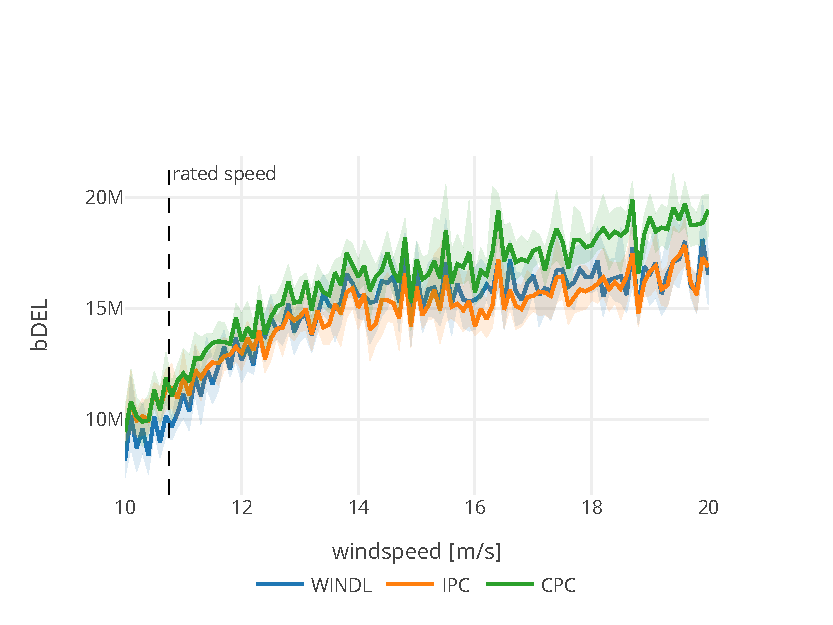
\includegraphics[width=\textwidth]{images/transfer_turbulent_bdel.pdf}
      \caption{blade-DELs against windspeed}
      \label{fig:transfer-turbulent-bdel}
  \end{subfigure}
  \begin{subfigure}[b]{0.48\textwidth}
      \centering
      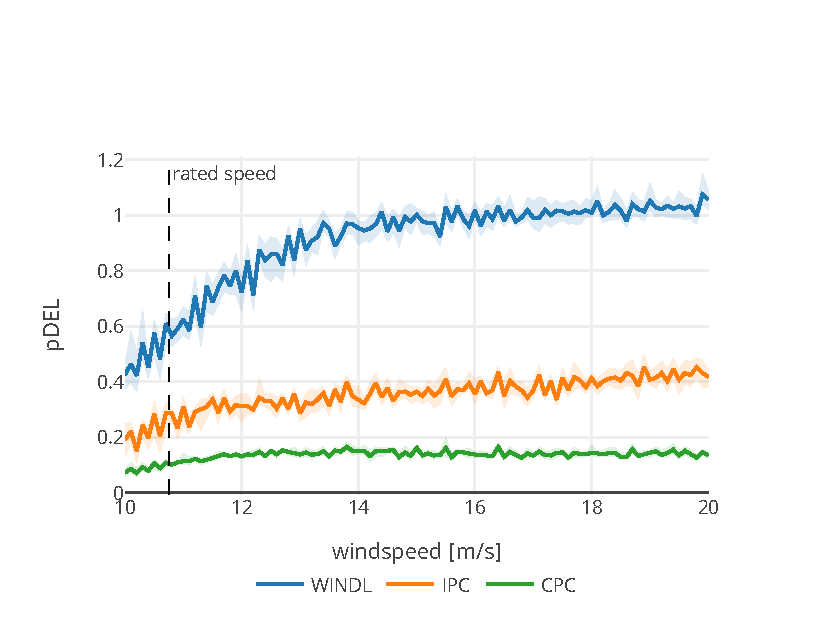
\includegraphics[width=\textwidth]{images/transfer_turbulent_pdel.pdf}
      \caption{pitch-DELs against windspeed}
      \label{fig:transfer-turbulent-pdel}
  \end{subfigure}
  \caption{The transfer performance of a model trained in the steady wind on a turbulent wind scenario, compared to IPC and CPC performance. Lower is better.}
  \label{fig:transfer-turbulent}
  % sac-steady-final, data_0, turb_reeval_468
\end{figure}

We measure the generalization performance of the best performing model from the steady wind (see Section \ref{section:results-steady-fatigue}) by evaluating it in the turbulent wind scenario. Note that the model has never seen a turbulent wind scenario during training. In Figure \ref{fig:transfer-turbulent}, we run WINDL on eight different turbulent seeds per wind speed for wind speeds between 10 and 20 m/s with a resolution of 0.1 m/s. For each metric, we plot a solid line for the mean value of performance across the turbulent seeds and a thin area around it for the bootstrapped 90\% confidence interval of these mean values. For both plots, lower values are better.
% Subfigure \ref{fig:transfer-turbulent-extreme} presents extreme values, which are calculated as the 99\% quantile value for blade bending moments. Subfigure \ref{fig:transfer-turbulent-rollout} presents an example rollout from the evaluation. 

While blade DELs in Subfigure \ref{fig:transfer-turbulent-bdel} largely match IPC performance, pitch wear values in Subfigure \ref{fig:transfer-turbulent-pdel} are on average 2.61 times as high as the IPC performance and 6.69 times as high as the CPC. In Figure \ref{fig:steady-sweep}, the same policy was able to outperform in terms of blade DELs while exhibiting the same pitch DELs. We also calculate extreme load values as the $.99$-quantile value for blade bending moments across the rollout. We find that WINDL exhibits 2.7\% higher extreme loads than the IPC but 7.55\% lower extreme loads than the CPC. 

\subsection{Turbulent To Steady}

\begin{figure}
  \centering
  \begin{subfigure}[b]{0.48\textwidth}
      \centering
      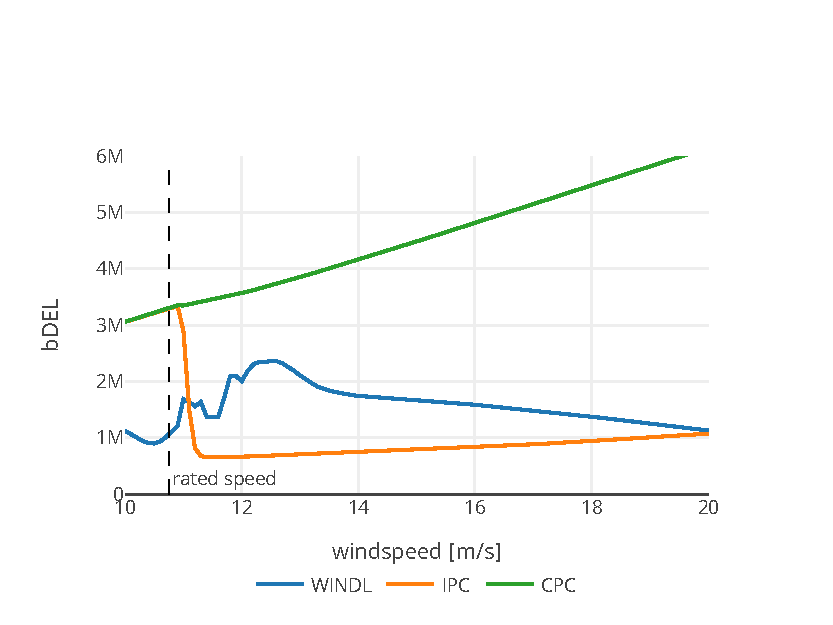
\includegraphics[width=\textwidth]{images/transfer_steady_bdel.pdf}
      \caption{blade-DELs against windspeed}
      \label{fig:transfer-steady-bdel}
  \end{subfigure}
  \begin{subfigure}[b]{0.48\textwidth}
      \centering
      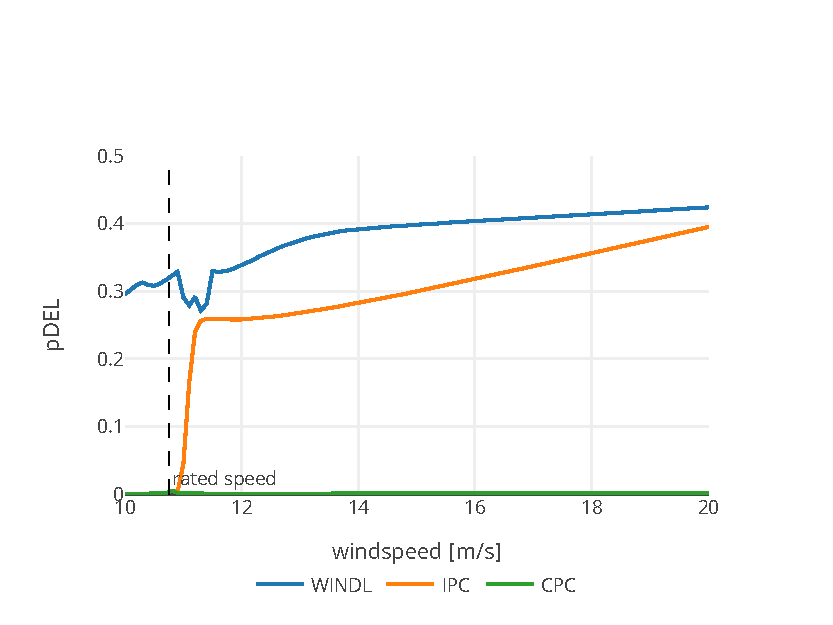
\includegraphics[width=\textwidth]{images/transfer_steady_pdel.pdf}
      \caption{pitch-DELs against windspeed}
      \label{fig:transfer-steady-pdel}
  \end{subfigure}
  \caption{The transfer performance of a model trained in the turbulent wind on a steady wind scenario, compared to IPC and CPC performance. Lower is better.}
  \label{fig:transfer-steady}
  % sac-turb-optim-1, data_42, steady_reeval_1430
\end{figure}

We measure the generalization performance of the adjusted model from the turbulent wind (see Section \ref{section:results-adjusted}) by evaluating it in the steady wind scenario. Note that the model has never seen steady wind during training. In Figure \ref{fig:transfer-steady}, we run WINDL on all wind speeds between 10 and 20 m/s with a resolution of 0.1 m/s. For both plots, lower values are better.

As visible in Subplot \ref{fig:transfer-steady-bdel}, the transfer-evaluated model performs worse than the IPC in terms of blade fatigue loads but better than the CPC. Above rated from 12-20 m/s, it produces 101\% more blade fatigue loads than the IPC but 65\% less than the CPC. At the same time, it exhibits higher pitch wear as visible in Subplot \ref{fig:transfer-steady-pdel}. Above rated, pitch wear is 25\% worse than the IPC. A phenomenon occurs at 11m/s, the onset speed of the torque controller, where both metrics show a dent. In the turbulent wind, transitioning this operating area happened only for small time periods during a gust, while resting at this operating area likely presents unseen challenges to the controller.

Around rated speed between 10 and 12 m/s, WINDL produces lower blade fatigue loads than both the IPC and the CPC, as visible in Subplot \ref{fig:transfer-steady-bdel} on the left side. Notably, it also produces lower fatigue loads than the WINDL policy that was trained in the steady wind in this area when compared to Figure \ref{fig:transition-bdel}. This comes at the price of a significant power loss. While the WINDL policy trained in the steady wind only loses 0.6\% power in the 10 - 12 m/s range, the policy trained in the turbulent wind loses 2.8\% compared to IPC and CPC. The policy trained in the steady wind did not have the capability of trading as much power for blade loads as the policy from the turbulent wind, as the hyperparameter set forbids the steady wind policy to set $c_S$ - the constant offset action. The turbulent policy can freely trade power for blade loads by setting $c_S$ to its maximum value.

\subsection{Discussion}
\label{section:results-transfer-discussion}


WINDL does not transfer well between wind scenarios. In the steady-to-turbulent direction, blade wear remains sensible, but pitch wear is far above the values of the IPC. In the other direction from turbulent to steady, WINDL produces worse pitch and blade wear than the IPC baseline above rated and loses significant amounts of power around rated. While both behaviors would likely not lead to immediate destruction of the turbine, operating a WINDL policy in a wind scenario for which it was not trained is not advisable.

The difference between the steady and turbulent wind scenarios is immense. We do not expect a controller to learn the extreme dynamics of turbulences only from the steady wind. Neither was our expectation for the controller to learn the gentle adjustments necessary to outperform in the steady wind while being subjected to heavy turbulences. However, the underlying dynamics of the turbine are the same, so generalization is not impossible. The shown case could be the most difficult generalization task for wind turbine environments. We do not evaluate generalization tasks that could be easier to solve, such as generalizing from lightly turbulent to strongly turbulent wind where stochastic elements are present in both scenarios.

We expect slightly better results upon utilization of generalization techniques such as dropout or deep neural nets, but we do not expect a drastic improvement. \citet{cobbeQuantifyingGeneralizationReinforcement2019} have shown common ML generalization tweaks to work, but did not record massive improvements. For their causal ladder model, \citet{pearlCausalInferenceStatistics2009} even prove that correct interventions generally require knowledge of the underlying causal model of the environment, as purely associational knowledge can be confounded. The knowledge encoded in the Q-function is purely associational. In a wind turbine, all parts are connected together, and as such, every part is a potential confounder for every other. For example, it is possible to excite a harmonic frequency of a part in a very specific scenario, which did not occur in all previously seen scenarios. Without the knowledge of the underlying model, this is impossible to predict. Additionally, relationships are often non-linear or stochasic, forming a generally difficult environment. The combination of the difficult wind turbine environment and the absence of modeling in our framework make good generalization performance unrealistic to achieve.

Modern wind turbine simulations are accurate models of the dynamics of a wind turbine \cite{martenQBladeModernTool2020}. Furthermore, there is at least some knowledge on the stochastic nature of turbulences \cite[Chapter 2.6.1]{burtonWindEnergyHandbook2011}. These models could be used for a model-based reinforcement learning approach in future work.

For a real-world application of the model-free WINDL, this means that an exhaustive evaluation set is crucial. All types of wind scenarios must be present in evaluation to build enough confidence in the performance of the algorithm, as relying on generalization performance is not advisable. An example of this benchmark could be the IEC 61400-1 standard \cite{internationalelectrotechnicalcommissionIEC61400120192019}, which defines a set of design load cases for a turbine. Furthermore, stability guarantees are a crucial argument for real-world application in addition to empirical performance. Proving stability guarantees is impossible without a model of the environment, and hence a switch to model-based RL methods such as the approach by \cite{berkenkampSafeModelbasedReinforcement2017} could be an option.

\section{Reward Function}
\label{section:results-reward}

\begin{summary}
This section investigates the suitability of the reward function to represent the quantities of interest. We investigate the components of the reward functions and find that they relate to their respective quantities of interest. Furthermore, we show that the magnitude of these components is not congruent with the effect they have on final policy performance. 
\end{summary}

We evaluate the training from Section \ref{section:results-adjusted}, which trains an adjusted policy in the turbulent wind to 1500 epochs (36M environment interactions). We only show the first part of the training to 10M environment interactions to improve the readability of the plots.

We introduce the optimization aims in Section \ref{section:background-optimization-aims} and describe how the reward function is a heuristic for these optimization aims in Section \ref{section:approach-reward-shaping}. While it would be mathematically possible to optimize DEL metrics directly, we use a reward function based on heuristics that can be computed for every timestep to give instantaneous feedback. It is desirable for these heuristics to exhibit optima in the same place of the parameter space as the underlying physical wear process. Hence, we expect the components of the reward function to reflect DEL metrics. Where the DEL metric is high, a high penalty should be applied to incentivize different behavior.

\subsection{Presentation}

\begin{figure}
  \centering
  \begin{subfigure}[b]{0.48\textwidth}
      \centering
      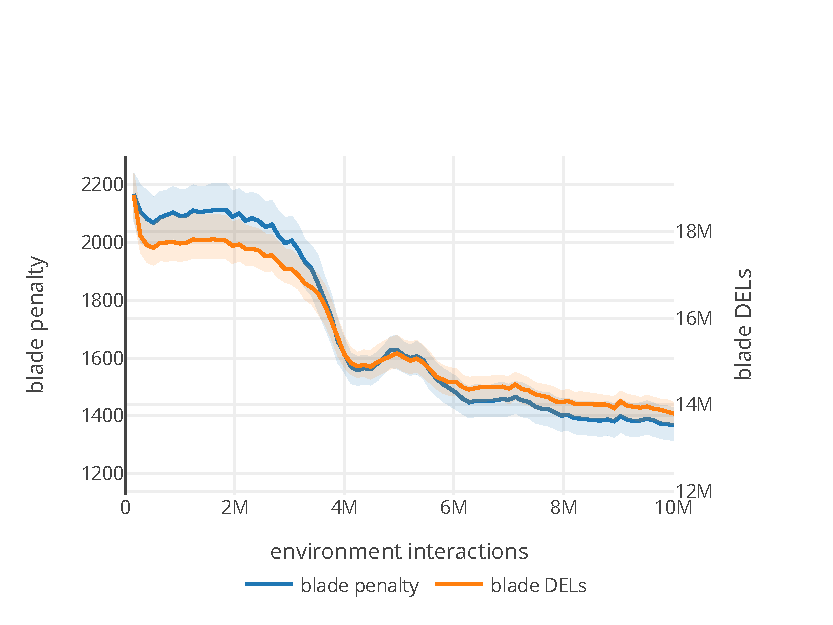
\includegraphics[width=\textwidth]{images/reward_analysis_blade.pdf}
      \caption{Blade penalty and DELs over training time}
      \label{fig:rc-blade}
  \end{subfigure}
  \begin{subfigure}[b]{0.48\textwidth}
      \centering
      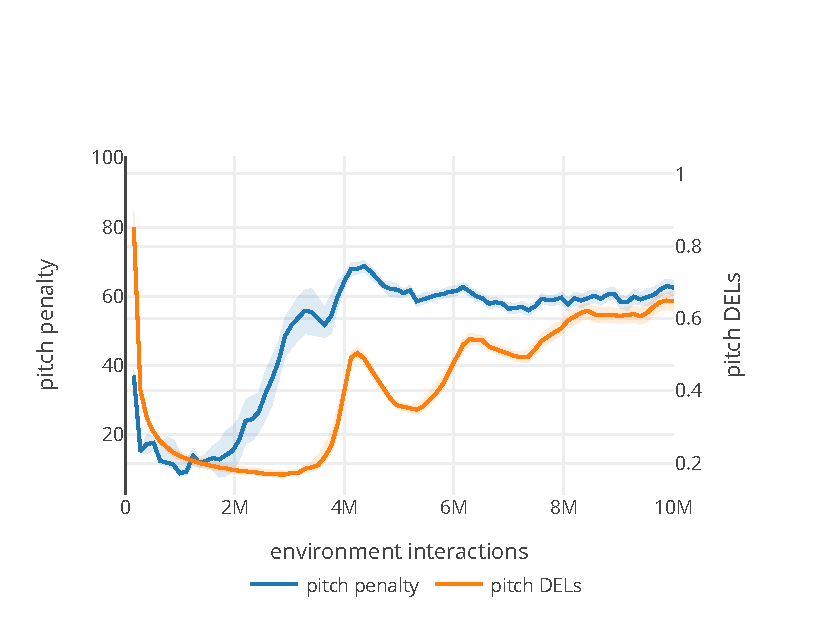
\includegraphics[width=\textwidth]{images/reward_analysis_pitch.pdf}
      \caption{Pitch penalty and DELs over training time}
      \label{fig:rc-pitch}
  \end{subfigure}
  \caption{Reward composition compared to DEL development over training time. The reward penalties for blades and pitch loosely match the DEL metrics of their component}
  \label{fig:rc}
  % sac-turb-optim-1, [], {'deterministic': True, 'mask_act': 'coleman-no-torque-s', 'discount': 0.99, 'qf_lr': 1e-4}, windspeed >= 12
\end{figure}

Figure \ref{fig:rc} shows the reward components over the course of a training plotted together with the relative DEL metrics of the same training run. The value plotted as blade penalty is the norm of the Coleman transformed blade bendings: $\rcoleman \sqrt{\tilde{c_s}^2 + {c_d}^2 + {c_q}^2}$. The value plotted as pitch penalty is calculated as $\rcolemanact \sqrt{{c_S}^2 + {c_D}^2 + {c_Q}^2}$. Note that both penalties are \textit{subtracted} from the reward function, so the agent optimizes towards lower values. Because of the different scales of reward components and DELs, two y-axes are used with the leftmost one corresponding to the reward component and the rightmost one to the DEL value of that turbine component. The constant offset $\rconst=1$ is omitted for brevity. Both plots show \ac{IQM} performance across eight wind speeds between 10 and 20 m/s and four training runs with different random seeds for each point on the x-axis. 

The pitch and blade penalty have different orders of magnitude. Blade penalties are around 20 times higher than pitch penalties. Despite the difference of one magnitude between the pitch reward and the blade reward, the pitch reward has an impact on final policy behavior. We observed that especially with lower discounting factors, increasing $\rcolemanact$ further lead to policies not doing anything in our hyperparameter search because the pitch penalty had a too great influence. The value shown here incentivizes pitch saving behavior in comparison to the naive training as shown in Section \ref{section:results-naive-turbulent}.

The curvature in the pitch penalty plot in Subfigure \ref{fig:rc-pitch} loosely matches the mirror of the curvature of pitch DELs. At 4M environment interactions, a peak in pitch DELs is accompanied by a small peak in pitch penalty, suggesting that this peak was captured by the reward function. An upwards trend with a small downwards peak in pitch penalty from 2M to 3.5M environment interactions is not visible in the DEL plot, suggesting that a phenomenon penalized by the reward function is not relevant for pitch DELs. Even though the pitch penalties stay relatively level above 4M environment interactions, pitch DELs increase in waves, suggesting another mismatch between pitch DELs and the pitch reward component.

The blade penalty as shown in Subfigure \ref{fig:rc-blade} very closely matches blade DELs. Peaks in both direction show both in the reward component and the DEL metric, suggesting that the reward component is a good heuristic for blade DELs. The general trend of blade DELs is downwards, meaning towards a better-performing policy with respect to the primary optimization aim.

\subsection{Discussion}

Counter to expectations, the algorithm does not weigh the pitch and blade component of the reward function equally. A pitch penalty one order of magnitude below the blade penalty is enough to incentivize pitch saving behavior, while increasing the pitch penalty further does not reduce pitch wear as shown in Section \ref{section:results-pb-trade-off}. We attribute this to the learnability of the two components. While pitch wear is directly caused by policy actions, blade wear is mostly caused by turbulence. Hence, learning the pitch penalty is easier, and a pitch penalty one order of magnitude smaller is sufficient to incentivize a behavioral change.

While the pitch penalty seems to only loosely match pitch DELs, the blade penalty reflects blade DELs well. This might partially explain the different success levels on minimizing blade DELs and pitch DELs. Each of the two penalties is constituted of the norm of a three-element vector, and the influence of the individual vector elements on these plots is not shown. While mainly penalizing pitch and blade wear, the reward function also serves to inhibit local maxima as described in Section \ref{section:approach-reward-shaping} through the inclusion of the $\tilde c_s$ and $c_S$ components. Inhibiting local maxima can cause movement in the penalty components that is not reflected in DELs. 

In total, our chosen reward function is a suitable metric for optimization through reinforcement learning. The instantaneous feedback enables easier learning across long trajectories, it does not exhibit local maxima that can be exploited, and it matches the optimization quantities at hand. Accumulating six signals into one does not throw off the Q estimation process, and enough signal-to-noise ratio is retained to train a Q function approximator.

In this chapter, we omit results from experimenting with other reward functions. We tried combinations of penalties for raw pitch travel, raw blade bendings, power loss, rotational speed fluctuation, exceeding maximum rotational speed, tower vibrations, and raw tower bendings. After lengthy searches for suitable coefficients, we settle for the Coleman-based reward function due to its simplicity.

\section{RL Algorithm Components}
\label{section:results-rl-components}

\begin{summary}
This section goes into detail on the different components of the reinforcement learning algorithm. We show the interaction of the Q-function and policy in general and investigate raw neural network outputs in detail. We find that the Q-function is flatter than expected within the action space bounds, which could be caused by the complex state domain of the wind turbine environment. Furthermore, we are unable to extract insights into the knowledge of the network from Q outputs. 
\end{summary}

We evaluate the training from Section \ref{section:results-adjusted}, which trains an adjusted policy in the turbulent wind to 1500 epochs (36M environment interactions).

As described in Section \ref{section:background-sac}, different components of the actor-critic algorithm interact to optimize the quantity of interest: expected discounted return. The critic, which is called Q-function throughout this work, aims to fit expected return for arbitrary states and actions. The actor, which is called policy throughout this work, aims to find the action that maximizes the Q-value for a given state. The Q-function is trained by using the Bellman backup from Equation \ref{eq:bellman-backup} in a recursive manner with separate target networks. To counteract overestimation bias, two Q-functions are used. The policy is trained by deriving a gradient through the more conservative of the two Q-functions, leading the policy towards a maximum in the Q-function curvature.

\subsection{Training Process}

\begin{figure}
  \centering
  \begin{subfigure}[b]{0.48\textwidth}
      \centering
      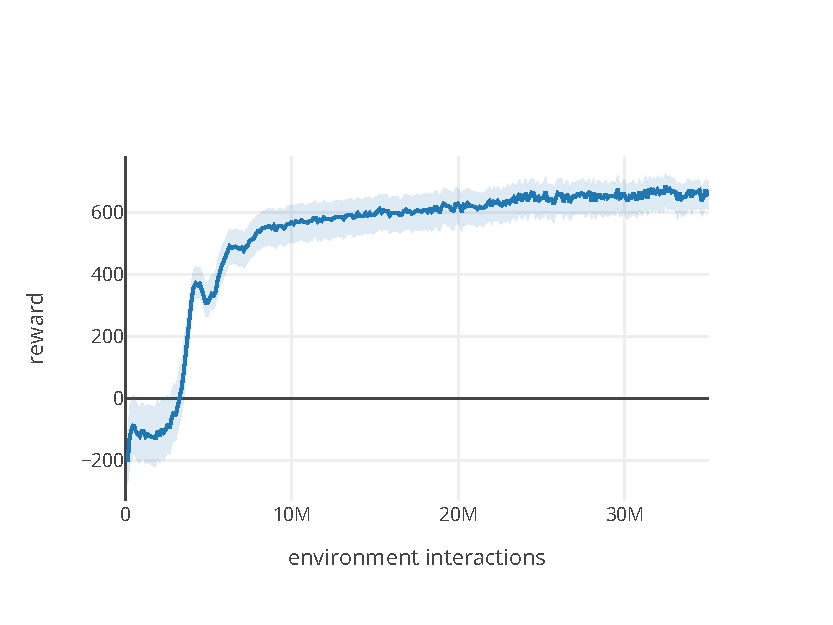
\includegraphics[width=\textwidth]{images/algocomps_reward.pdf}
      \caption{Reward over training time}
      \label{fig:training-reward}
  \end{subfigure}
  \begin{subfigure}[b]{0.48\textwidth}
      \centering
      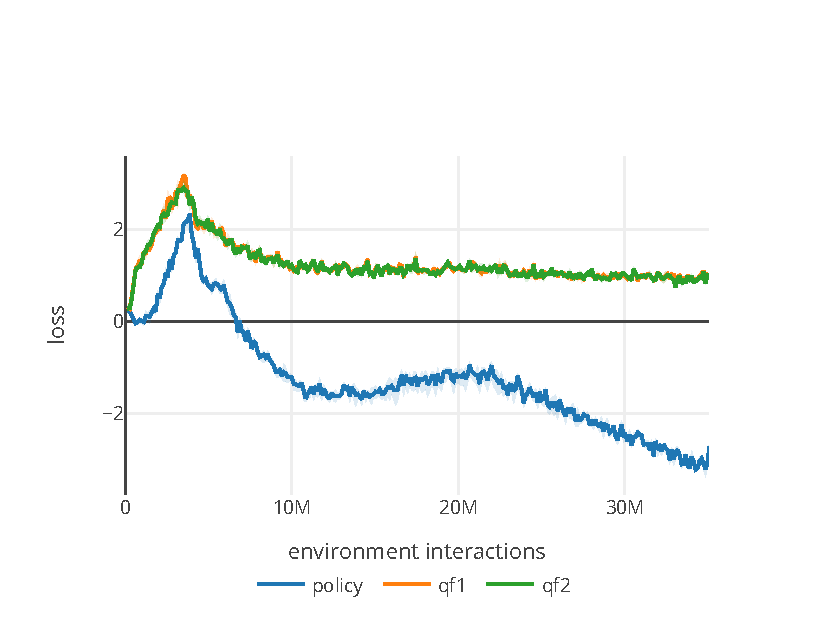
\includegraphics[width=\textwidth]{images/algocomps_losses.pdf}
      \caption{Losses over training time, policy loss scaled by a factor of 0.2 to fit the plot axis}
      \label{fig:training-loss}
  \end{subfigure}
  \caption{Reward and loss development over training time}
  \label{fig:training}
  % sac-turb-optim-1, [], {'deterministic': True, 'mask_act': 'coleman-no-torque-s', 'discount': 0.99, 'qf_lr': 1e-4}, windspeed >= 12, policy loss magnified * 0.2
\end{figure}

Figure \ref{fig:training} shows the losses of the Q-functions and policy over the training time, together with the average reward of the policy. The reward function is discussed in Section \ref{section:results-reward}, where the reward composition for the first 8M environment interactions is shown. Note that the policy loss is not a loss in the traditional sense of a difference between predictions and target values. It is the output of the Q-function for the action generated by the policy, meaning it is an estimate of the return that the policy would achieve with the current action, as shown in Equation \ref{eq:soft-policy-update}. Because the deep learning library in use (pytorch), only supports gradient \textit{descend} while the optimization aim in Equation \ref{eq:soft-policy-update} is a \textit{maximization} objective, the output is multiplied by -1. Hence, negative policy loss stems from a positive Q estimate.

In the first part of the training to 8M environment interactions, the reward function changes most, whereas after 8M environment interactions, it slowly rises to its plateau value of around 650. Around 4M environment steps, a bump in the reward function is visible. Also, around 4M environment steps, both the policy and Q-function losses peak. The policy loss decreases with a stagnation between 13M and 21M environment interactions, while the Q-function losses stagnate.

We observe a peak similar to the one at 4M environment steps throughout all of our training process. Different hyperparameter choices move, but do not remove the period of rising losses at the beginning. This peak coincides with a bump in the reward function, where performance degrades for a short period of time. We investigate this bump and find a strong correlation with policy entropy - the higher the starting entropy target $\alpha$, the more pronounced this bump is.

We believe the exploration strategy to be the cause for this bump. To enable exploration, the policy has a gaussian noise component that is maximized through the maximum-entropy framework. This gaussian noise component is detrimental to the wind turbine, as the turbine reacts to the noise applied to it. The effect of this noise is not captured by the Q-function until around 4M interactions, when the negative effect of entropy is starting to be modeled. Earlier modeling of the negative effect is inhibited by the maximum-entropy framework, which incentivizes \textit{maximal} entropy that counters the \textit{minimal} entropy, which is optimal for the wind turbine. Only when policy performance can not be optimized through other means, the algorithm starts to shift attention to the entropy part. From then on, policy performance becomes slightly better with the decreasing $\alpha$ component. The exploration-exploitation trade-off is especially tricky in wind turbine reinforcement learning, as entropy is required for exploration to find better policies, but having entropy causes worse policies. Learning to distinguish between these two counteracting causes is sample-intensive and requires 4M environment interactions. For comparison, \citet{haarnojaSoftActorCriticOffPolicy2018} only train to 3M interactions to solve most gym environments.

\subsection{Q-Function Curvature}

We observe a phenomenon where most of the Q-Function curvature lies outside of the action space.

\begin{figure}[hbt]
  \centering
  \begin{subfigure}[b]{0.48\textwidth}
      \centering
      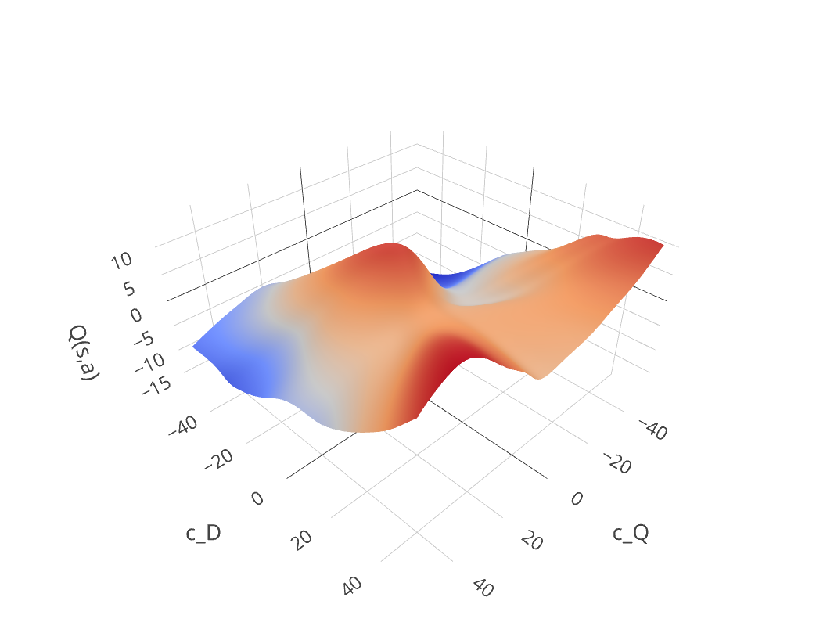
\includegraphics[width=\textwidth]{images/frame_zoomout.pdf}
      \caption{Q-function zoomed out for t=0}
      \label{fig:qf-zoom}
  \end{subfigure}
  \begin{subfigure}[b]{0.48\textwidth}
    \centering
    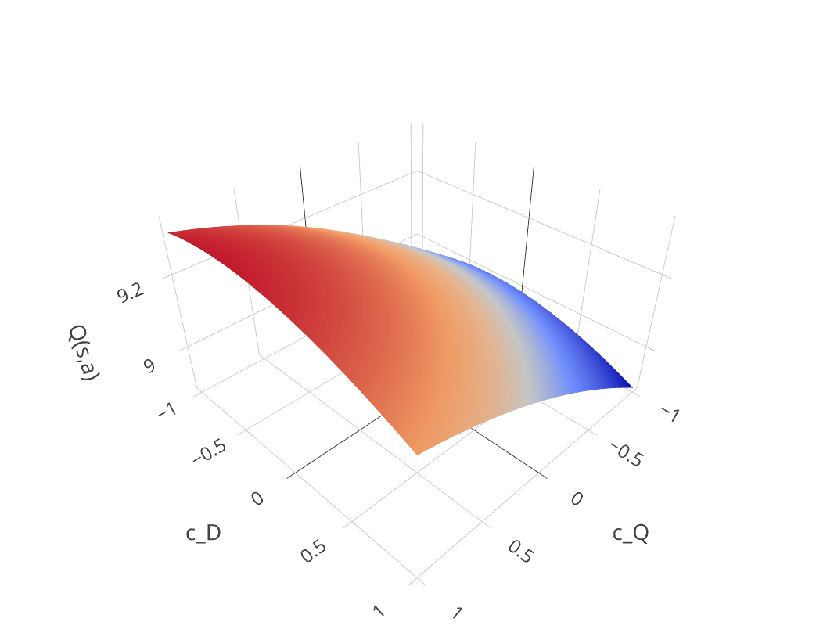
\includegraphics[width=\textwidth]{images/frame_0.pdf}
    \caption{Q-function at t=0}
    \label{fig:qf-t0}
    % traj_idx 879
  \end{subfigure}
  \begin{subfigure}[b]{0.48\textwidth}
    \centering
    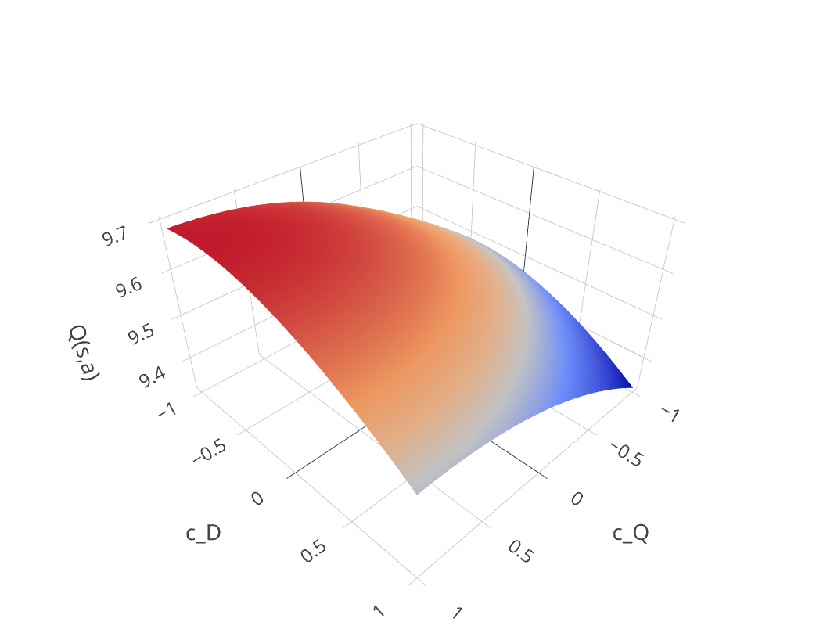
\includegraphics[width=\textwidth]{images/frame_1.pdf}
    \caption{Q-function at t=1}
    \label{fig:qf-t1}
    % traj_idx 880
  \end{subfigure}
  \begin{subfigure}[b]{0.48\textwidth}
    \centering
    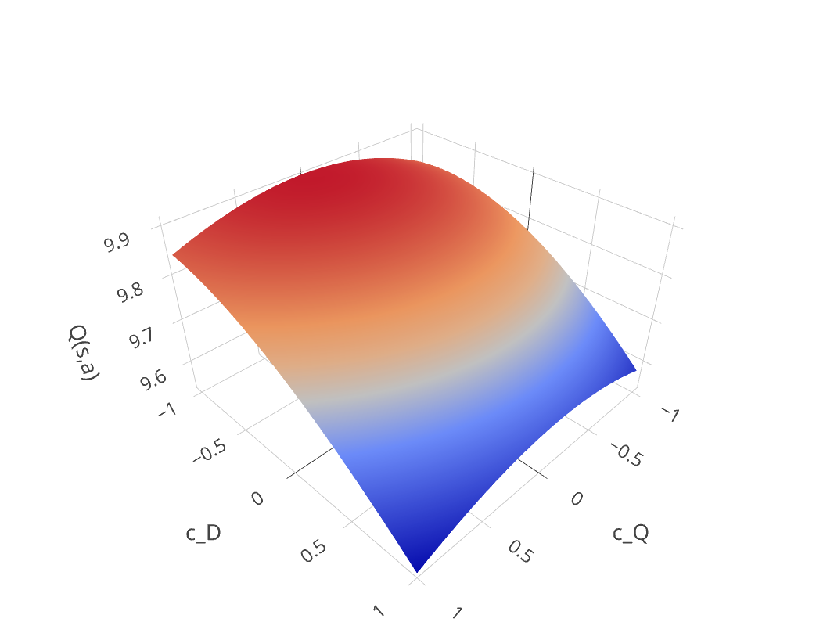
\includegraphics[width=\textwidth]{images/frame_2.pdf}
    \caption{Q-function at t=2}
    \label{fig:qf-t2}
    % traj_idx 881
  \end{subfigure}
  \caption{Q-function curvature across two action space dimensions $c_Q, c_D$}
  \label{fig:qf}
  % sac-turb-optim-1, data_1, eval-1545, eval run 2
\end{figure}

Figure \ref{fig:qf} shows the Q-function values across two dimensions of the action space, $c_Q, c_D$. Section \ref{section:approach-postprocessing} describes these two to be the pitch action difference across the tilting and yawing axes of the rotor plane. In Subplots \ref{fig:qf-t0} \ref{fig:qf-t1} \ref{fig:qf-t2} they are constrained to their allowed range before postprocessing of [-1, 1], while in Subplot \ref{fig:qf-zoom} the Q-function is evaluated for hypothetical actions in the range [-50, 50]. Note that during training, the Q-function has only seen the range [-1, 1]. Subplots \ref{fig:qf-t0} \ref{fig:qf-t1} \ref{fig:qf-t2} show the original Q-function as used during policy optimization for three consecutive time steps.

In the three plots, the curvature of the Q-function is minimal; they are almost a flat plane. The maxima lie at the border of the action space, which should incentivize the policy to produce actions at the border of the action space. For Subplot \ref{fig:qf-t0} and \ref{fig:qf-t1}, the maximum lies at $c_Q=1, c_D=-1$ and for \ref{fig:qf-t2} it is at $c_Q=0.1, c_D=-1$. These are both drastic actions and drastic change across a single timestep. The actual actions taken by the policy are however $t_0: [c_Q=-0.03, c_D=0.09]$, $t_1: [c_Q=-0.05, c_D=0.07]$, $t_2: [c_Q=-0.09, c_D=0.6]$, which are more sensible and gentle actions than what the Q-function suggests. Furthermore, the zoomed-out version in Subplot \ref{fig:qf-zoom} exhibits a landscape that is closer to our expectations, where there are multiple peaks and valleys for good and bad actions. This shows that the Q-function is able to create such a landscape in principle, meaning it is not underparametrized. However, it does not do this in the action space. In the following passages, we make guesses for the two questions introduced by this phenomenon: what causes the Q-function to have such a flat curvature inside of the action space boundaries, and how does the policy learn to act sensibly nevertheless.

We theorize feature coadaptation \cite{kumarDR3ValueBasedDeep2021} to be the cause of the flat policy curvature. In their work, \citet{kumarDR3ValueBasedDeep2021} describe feature coadaptation to be a phenomenon in offline RL, where the last-layer activations of the Q-function for two adjacent time steps are very similar, i.e. they have a high dot product. We measure feature coadaptation for the shown plots, and get 173.2 for $t_0$ to $t_1$ and 173.3 for $t_1$ to $t_2$. Compared to the results in \cite{kumarDR3ValueBasedDeep2021}, this is low, especially after the training time for this checkpoint. Hence, we discard the theory of feature coadaptation to be at the cause of the flat Q-function phenomenon.

Furthermore, we theorize the nature of the wind turbine environment to cause the flat curvature of the action space. The stochastic wind is the biggest factor to returns, while the actions of the policy can only make a minor difference. Even with a perfect load control policy, loads will be far from zero, and reward will still fluctuate with state changes. Hence, the Q-function learns to adapt mainly to the state input and partially disregard the action input. More fit can be achieved by focussing curvature on the state dimensions than to focus on the action dimensions. Problematically, the action dimensions are the quantity of interest to optimize the policy, while knowing the expected return along the state dimension is of less interest for Q-function based RL. Other algorithms like \ac{PPO} \cite{schulmanProximalPolicyOptimization2017} model a value function, which purely encodes state-based expected returns and thus could potentially avoid this problem.

The second question is why the policy still learns to output sensible actions, which are not at the boundary of the action space all the time. We theorize two phenomena to be the cause for this, the smoothing effect of stochastic gradient descend and policy smoothing through CAPS regularization. Stochastic gradient descend performs gradient computations based on multiple samples, in this case, 256. As the Q-function plane curves in different directions over a single batch, the smoothing effect of stochastic gradient descend brings the policy to a middle ground between the extreme values suggested by the Q-function. Furthermore, CAPS policy smoothing regularizes the policy to not exhibit drastic changes from one state to the next. Extreme actions as suggested by the Q-function in the above plots would need to be suggested consistently over a long time-span for the regularized policy to converge to them. However, the Q-function changes its orientation rapidly and does not leave time for the policy to reach a border.

Likely, the smoothness of the policy, together with the relatively low entropy used for exploration, further exacerbate the flat Q-function phenomenon. The Q-function rarely sees actions at the action space boundary, because the smooth policy produces more conservative actions. The Gaussian noise applied to it is too low to ever sample an action at the border of the action space, so the Q-function does not know from samples how these actions would play out and overestimates them due to the inherent overestimation bias in Q-learning \cite{fujimotoAddressingFunctionApproximation2018}.

Concludingly, it is likely that multiple phenomena are at play. Due to the black-box nature of neural networks, it is difficult to pinpoint problems, and the complex interaction of policy and Q-function in actor-critic RL only complicates this. However, human interpretability is not a common benchmark for RL algorithms. Ongoing work in the field of causal reinforcement learning \cite{bareinboimCausalReinforcementLearning2020} aims to train more insightful policies which can be interpreted. With our current knowledge, we can only formulate guesses to the underlying mechanisms that cause this phenomenon.

\subsection{Discussion}

While we can demonstrate the high performance of WINDL by benchmarking it, we can not extract knowledge to \textit{why} it is doing what it is doing. 

In this section, we have shown the complex interplay between the components of the reinforcement learning algorithm in action. Due to the uninterpretable nature of neural networks and exacerbated by the complex interplay of policy and Q-function, interpreting the learned policy is difficult. The Q-function only works in conjunction with the policy, and questions such as \textit{what if} a different policy was at play can not be answered to satisfaction. This is a fundamental limitation of current approaches in model-free reinforcement learning, which maximize policy performance but do not output interpretable signals for a human to judge the level of understanding obtained. While for supervised learning, multiple publications have gained insights into the inner workings of the neural net \cite{zeilerVisualizingUnderstandingConvolutional2013} \cite{mordvintsevDeepDream2015}, such results are sparse for reinforcement learning. The field of causal reinforcement learning \cite{bareinboimCausalReinforcementLearning2020} aims to tackle this problem but has yet to prove its potential.

For the application of WINDL, such interpretability would be desirable. It would form a justification basis in addition to the benchmarks, which could convince wind turbine manufacturers to implement a RL-based control policy. Furthermore, it could allow fine-tuning by precisely changing those parameters, that lead to a certain behavior. Currently, the only option for tuning WINDL is through the choice of hyperparameters, which is more of a trial-and-failure approach than directed fine-tuning.

\chapter{Related Work}
\label{ch:related-work}

In this chapter, we present related work and how our approach compares to these. We applied a smooth continuous control reinforcement learning algorithm with amendments for the use in a rotating coordinate space to solve wind turbine load control, hence we evaluate other works solving wind turbine load control with a specific focus on approaches incorporating machine learning. Specifically, works by \citet{coqueletBiomimeticIndividualPitch2020} and \citet{asgharniaLoadMitigationClass2020} fall into this category, and we give a summary of them in Sections \ref{section:related-kotlett} and \ref{section:related-asgharnia}. There is a high number of works solving wind turbine load control without the use of machine learning, we present the work by \citet{jonesOvercomingFundamentalLimitations2018} as a representative in Section \ref{section:related-jones}. Our approach directly builds upon, evaluates against, and competes with the ideas of \citet{bossanyiIndividualBladePitch2003} as presented in Section \ref{section:background-ipc}. Due to the exhausive referencing throughout the rest of the work, we will not reference traditional \ac{IPC} approaches in this chapter. 
% Other works that fall into this category include \todo{spam stuff into this list}:

% \begin{itemize}
%   % \item \citet{bossanyiIndividualBladePitch2003} and \citet{bossanyiFurtherLoadReductions2005} wrote the foundational paper for individual pitch control, discussed in background section \ref{section:background-ipc}
%   \item \citet{larsenActiveLoadReduction2005} propose different input sensors which measure flow as an IPC basis
%   % \item \citet{jonesOvercomingFundamentalLimitations2018} work with local inflow sensors on the blades to improve IPC performance.
% \end{itemize}

% We refrain from summarizing these works, as they are close or comparable to other works presented.

While RL for wind turbine load control has not seen a high amount of published works, other control aims in the field of wind turbines have been researched.
\begin{itemize}
  \item \citet{hosseiniImprovingResponseWind2020} learn PID parameters through \ac{RL} with the aim of output power smoothing
  \item \citet{chenReinforcementbasedRobustVariable2020} stabilize rotor speed through a \ac{RL} collective pitch controller
  \item \citet{zhangReinforcementLearningBasedStructural2020} stabilize floating turbines through \ac{RL}
  \item \citet{saenz-aguirreArtificialNeuralNetwork2019} implement \ac{RL}-based active yaw control
  \item \citet{zhaoCooperativeWindFarm2020} use \ac{RL} for wind farm control
  \item \citet{padullaparthiFALCONFArmLevel2022} use \ac{RL} for wind farm control
\end{itemize}
Each of this works has another optimization goal than our approach, and due to that a different choice of measurements, RL architecture and evaluation metrics. Hence, these works are not in the scope of this chapter.

Lastly, our approach is comparable to any continuous control reinforcement learning applications in a rotating coordinate space, independent of the actual field of application. To us, no such applications in a rotating system are known outside the field of wind turbine control. The more general field of continuous control reinforcement learning applications offers a vast amount of published work, but the intersections with our work are slim and comparability is not given. Hence, this boarder field is out of the scope of this chapter.






% \item \citet{yangIndividualPitchController2016} implement a fuzzy logic based pitch controller
% \item \citet{yilmazPitchAngleControl2009} train a supervised model to match a known pitch signal



% Some examples for further applications of \ac{RL} outside the field of wind turbine control are
% \begin{itemize}
%   \item \citet{leeAlgorithmAutonomousPowerincrease2020} control nuclear power plant startup with \ac{RL} 
%   \item \citet{hwangboControlQuadrotorReinforcement2017} control a quadrocopter through \ac{RL}
%   \item \citet{piLowlevelAutonomousControl2020} control a quadrocopter through \ac{RL}
%   \item \citet{reddyGliderSoaringReinforcement2018} control a glider through \ac{RL}
% \end{itemize}

\section{Biomimetic Individual Pitch Control For Load Alleviation}
\label{section:related-kotlett}

This section evaluates \citet{coqueletBiomimeticIndividualPitch2020}. Their general aim is to reduce wind turbine fatigue loads with an alternative strategy to the common Coleman transformation based IPC. As seen in Figure \ref{fig:coquelet-schema} they utilize a three-level pipeline for their setup. The flow sensing component is a preprocessing component, which evaluates sensory inputs. The central pattern generator transforms the discrete RL signals into continuous individual pitch angles. The \ac{RL} component in the middle outputs amplitude and phase parameters to the oscillators. They utilize the algorithm \ac{SAC} with a discrete action space.

\begin{figure}
  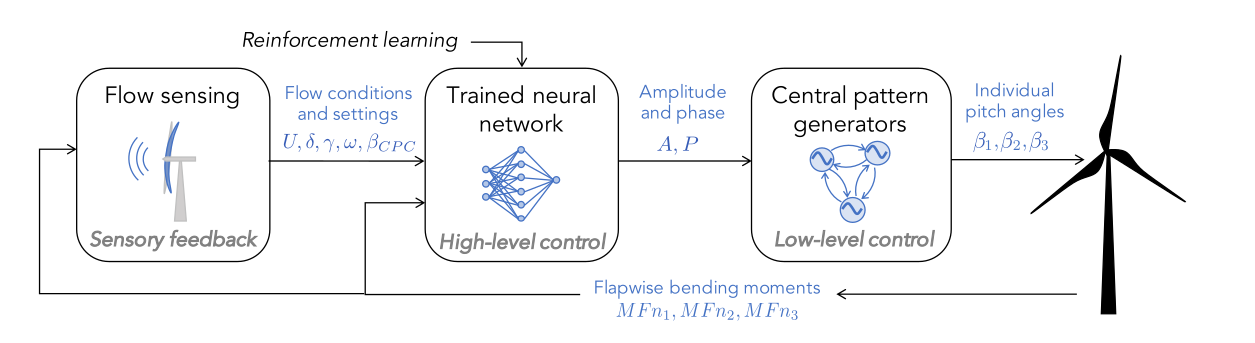
\includegraphics[width=\textwidth]{images/Coquelet-schema.png}
  \caption{The schema of the biometric \ac{IPC} by \citet[Figure 1]{coqueletBiomimeticIndividualPitch2020}}
  \label{fig:coquelet-schema}
\end{figure}

They minimize the distance between the highest and lowest blade bending moment as in equation \ref{eq:coquelet-reward}:
\begin{equation}
  r(s, a) = (\max_i(\soopbend_i) - \min_i(\soopbend_i)^{-2}
  \label{eq:coquelet-reward}
\end{equation}

Their training environment consists of a lower accuracy \ac{BEM} model of the wind turbine, while their evaluation happens in a higher quality \ac{VPM} based simulation. They test on the NREL 5MW reference turbine \cite{jonkmanDefinition5MWReference2009}. Instead of directly outputting pitch angles, the \ac{RL} agent outputs phase and amplitude settings for biometric oscillators which generally follow the form of equation \ref{eq:coquelet-oscillator}:

\begin{equation}
  \ddot{x} = \kappa_x (\frac{\kappa_x}{4}(X - x) - \dot{x})
  \label{eq:coquelet-oscillator}
\end{equation}

where $x$ is the output from the \ac{RL} agent, $\kappa_x$ is a gain constant, $X$ is a target value for $x$ to smoothly converge to and $\dot{x}$ and $\ddot{x}$ being the first and second derivative of the variable. This formula is used to compute offset, amplitude and phase of a oscillation: $\apitch = x_{\text{offset}} + x_{\text{amplitude}} \cos(x_{\text{phase}} + \sazi)$. While amplitude and phase are output from the \ac{RL} agent, the offset is taken as the pitch output from a traditional collective pitch controller.

\begin{figure}
  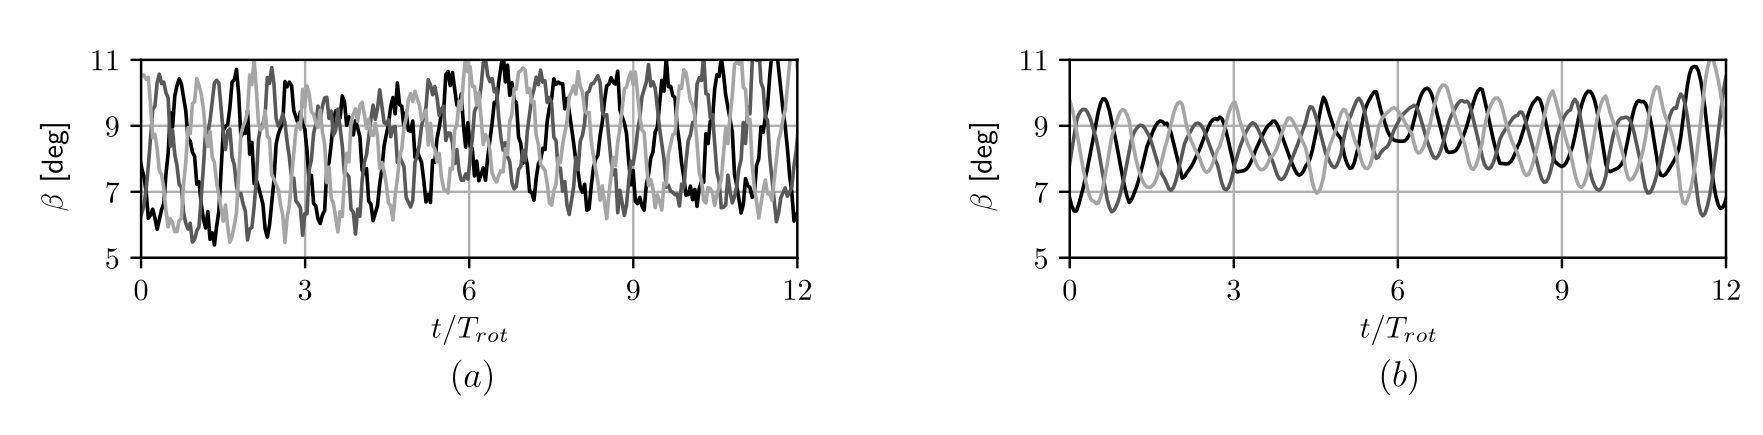
\includegraphics[width=\textwidth]{images/Coquelet-results.png}
  \caption{A rollout of a traditional Coleman-Transform based IPC (a) versus their biometric \ac{IPC} (b) by \citet[Figure 5]{coqueletBiomimeticIndividualPitch2020}}
  \label{fig:coquelet-results}
\end{figure}

\begin{table}
  \centering
\begin{tabular}{c c}
\hline
Method & Equivalent bending moments [MNm] \\
\hline
CPC & 2.54 \\
CT-IPC & 0.99 \\
BI-IPC & 1.40 \\
\hline
\end{tabular}
\caption{Equivalent bending moments from a collective pitch controller (CPC), a Coleman-Transformation based IPC (CT-IPC) and their biometric IPC (BI-IPC), by \citet[Table 1]{coqueletBiomimeticIndividualPitch2020}}
\label{table:coquelet-results}
\end{table}

To evaluate their results, they calculated equivalent bending moments, a measure which calculates a material-specific fatigue load equivalent to a seen trajectory \cite{blasquesMeanLoadEffects2013}. In Table \ref{table:coquelet-results}, their results show that their biometric IPC reaches less fatigue load reduction than a Coleman-Transformation based IPC but more than a collective pitch controller. They argue however, that their rollouts are smoother than the IPC as seen in Figure \ref{fig:coquelet-results}, thus forming a compromise between the CT-IPC and CPC. Furthermore, they claim more input information such as local blade flow velocities to allow for further blade load reduction, but do not show experiments to prove this.

\subsubsection{Direct Comparison}

This work is similar to our work in many terms. It uses similar methodology and similar inputs to solve the same problem. However, they optimize a different turbine model and different wind inflow conditions, hence direct comparability is not necessarily given.  As in our work, they use the reinforcement learning algorithm \ac{SAC} and utilize common wind turbine sensors as neural inputs. In contrast to our approach, they incorporate wind flow information. Compared to our results, they achieve less strong blade load reductions but also less strong pitch load increases, hence they trade pitch and blade loads differently. This is due to several factors.

Firstly, they operate in a discrete action space. While policies in a discrete action space tend to easier to train, they lack expressivity. It requires significant post-processing efforts to translate discrete actions to continuous smooth pitch angles. They utilize biometric oscillators to perform this translation. These oscillators produce gentle and smooth outputs even with a discrete input, but the possibilities of the reinforcement learning agent are limited strongly. Developing a pitching strategy with rich spectral contents on high frequencies, as observed in our work, is inhibited by the smoothing of the biometric oscillators. Operating directly in the continuous space like in our work offers more flexibility regarding the learnt policy. 

Secondly, they utilize a linearized model of the wind turbine to train their policy and a simulated environment to evaluate. By using the linearized model for training, they trade lower training complexity for lower learning potential. The partially non-linear aspects of the wind-turbine model are masked away, and some optimization potential is lost.

Third, they utilize a reward function which we briefly revisited during our experimentation. They penalize the squared difference between the highest and smallest bending moment, effectively incentivizing the bending moments to stay close to each other in each time frame. This does not penalize poor mean bending moments. For example low frequency oscillations, where all bending moments oscillate together on the tower eigenfrequency, are undetected by this reward. Also, extreme loads are undetected. However, due to the few terms, their reward function is compact and likely easier to learn than ours.

Congruent to our findings they conclude that RL is in principle able to optimize the wind turbine environment. Through the heavy filtered biometric oscillators, their policy is constrained to smooth actions and has less potential of damaging but also less potential of optimizing the turbine than in our work. In contrast to us, they do not outperform their IPC baseline with respect to the primary optimization metric blade loads.

\section{Load Mitigation Of A Class Of 5-MW Wind Turbine With RBF Neural Network
Based Fractional-order PID Controller}
\label{section:related-asgharnia}

This section evaluates \citet{asgharniaLoadMitigationClass2020}. They build a set of different PID-based collective pitch controllers for the NREL 5MW reference turbine \cite{jonkmanDefinition5MWReference2009} and evaluate them with respect to different metrics. In traditional controller design, a linearized model of the wind turbine is assumed and used as a tuning reference for PID parameters. Due to the linearity of the model, a closed form solution to the PID parameters can be found \cite[Eq 12 - 22]{asgharniaLoadMitigationClass2020}. This closed form solution yields different results for different operating wind speed, i.e. the optimal set of parameters to a PID controller depends on the speed of the incoming wind.

They build upon a common technique in wind turbine control design called gain scheduling. For this, a different set of parameters $(K_p, K_i, K_d)$ is used for different wind speeds. Obtaining robust wind speed measurements is nontrivial, as direct wind speed measurements by an anemometer are noisy. Anemometers are usually placed downstream of the rotor and thus experience wake effects from the passing blades. Furthermore, they only offer a point estimate of the wind speed at the nacelle, while the speed at the blade tips can be very different. Thus, they train a Radial-Basis-Function Neural Network to output the correct set of PID parameters based on wind turbine state. Concretely, they use rotational speed, output power and pitch angle. This training happens in a supervised fashion, as the wind turbine state for a given wind speed is known and the wanted PID parameters for a set of wind speeds were computed beforehand. Additionally, they utilize fractional order PIDs, which are similar to traditional PID controllers but with an additional parameter to the integration and derivation constant \cite[equation 24]{asgharniaLoadMitigationClass2020}.

They evaluate with respect to generator error (how far the generator output deviates from a wanted setting), pitch actuation, tower fore-aft torque and out-of-plane blade bending moments. For each scenario, they calculate \ac{RMS} values for their metrics in five different wind speeds with different wind noise levels. Their top performing variant, the FOPID showed 19.3\% less generator error than a baseline PID without a neural network, 22.4\% less pitch actuation rate, 13.3\% lower tower fore-aft acceleration and 19.7\% less out-of-plane bending moment. With this, they significantly outperform the baseline collective pitch controller, showing that a more intelligent actuation strategy has the potential of reducing blade, tower and pitch actuator loads at the same time. The \ac{RMS} metric is not directly comparable with other works like \citet{coqueletBiomimeticIndividualPitch2020} or \citet{bossanyiFurtherLoadReductions2005}, which calculate \acp{DEL}. However, it can be assumed that this collective strategy is an improvement over previous collective strategies. A collective pitch strategy has the advantage of being applicable to turbines which can not actuate their blades individually. Furthermore, it is imaginable to combine the FOPID with a load minimizing IPC, further reducing blade loads at the expense of extra pitch travel. 

\subsubsection{Direct Comparison}

In contrast to this work, this work does not utilize reinforcement learning, but a supervised framework to train a neural network to set PID parameters. Supervised learning is less complex, as it does not have to perform value approximation to then derive a policy from it, but directly uses human knowledge about optimal outputs based on wind turbine operating state inputs. This allows easier analysis of the approach and more security for real world applications. However, security guarantees are lower than those of traditional PID based works which can calculate a safety margin in closed form, as the neural network is still essentially a black box. The results are not directly comparable to our work due to two factors, first the use of a different evaluation metric, but more importantly, the fact that their work tackles collective pitch control instead of individual pitch control. Expected load reductions of collective pitch are significantly lower than those of individual pitch control at the benefit of reduced actuation complexity. Furthermore, a CPC policy can not reduce asymmetric rotor loads, while an IPC policy can. This difference makes a direct comparison of loads unsuitable. More generally, it can be stated that the use of machine learning techniques has leveraged higher optimization yields in this case, similar to our results.


\section{Overcoming Fundamental Limitations Of Wind Turbine Individual Blade Pitch Control With Inflow Sensors}
\label{section:related-jones}

This section evaluates the work of \citet{jonesOvercomingFundamentalLimitations2018}. Though this is not based on machine learning, it is a very promising method for load reduction.

Their key selling point is an \ac{IPC} design based on additional blade-local lift estimations. These lift forces can be inferred from pressure measurements using pitot tubes in the blades, effectively measuring local angle of attack and incoming air speed. When a gust hits the blade, these sensors immediately detect the higher load and can initiate a pitch reaction earlier than possible for a normal IPC. A normal IPC has to wait until the bending moments are at a high enough level to trigger a PID response, which is a long time on a modern wind turbine. Through a cascaded IPC design, which adds extra pitch actions inferred from inflow sensors to the IPC actions, they reach faster reaction times and stronger reactions.

The cascaded IPC exhibits better blade wear than the state-of-the-art, reducing blade DELs by ca 10\% in turbulent wind compared to their IPC baseline, but at the expense of higher pitch travel. The impact on extreme loads is relatively large, reducing maximum loads during an example wind shear by a factor of 2.5 with increased pitch travel by a factor of 2. 

\subsubsection{Direct Comparison}

A direct comparison is difficult, as they evaluate a single design load case with a wind shear and we evaluate in turbulent and steady wind. Through the single load case, load reductions are difficult to assess, as the load case could be not representative of a turbine life. However, their cascaded IPC exhibits lower blade loads at the cost of higher pitch travel, which is similar to our result. In the design load case shown, they reach a significant extreme load reduction an order of magnitude above the reduction provided by WINDL on average.

The authors argue that \ac{BRBM} sensors do not exhibit enough bandwidth to reach higher blade load reductions through the \ac{IPC} strategy, and other sensors like inflow sensors are needed instead. We show in our work that a non-linear neural policy is able to achieve further blade load reductions without using inflow sensors sensors but only using traditionally installed sensor inputs. In our case, these advancements have to do with the way the information is processed in the controller, hence we are able to overcome the fundamental bandwidth limitation partially. We assume that through the integration of advanced sensors like inflow sensors, also the WINDL policy could be improved as it receives more information about the surrounding flow.

Through the PID based IPC design, they can calculate a mathematical safety margin, whereas the WINDL policy can only be evaluated empirically to be safe. Such a safety margin is an important guarantee and likely a critical factor towards real world adoption.

\chapter{Conclusion}
\label{ch:conclusion}

This chapter summarizes the most notable results and concludes the potential impact of this work. Furthermore, it presents ideas for future work.

\section{Summary}

In this work, we successfully applied the methodology of reinforcement learning to the field of wind turbine load control. The controller learned the fundamental control mechanism that work for the turbine without prior knowledge of the model. It has a better performance to the popular IPC strategy, depending on the considered metric.

We demonstrate WINDL to be capable of learning a potent policy for the easier steady wind scenario, where it reduced blade equivalent loads from the current state-of-the-art by 54.1\%, introducing only 3.8\% more pitch equivalent loads. Also, we showed that through adjustment of hyperparameters, WINDL can bring a significant advancement in the turbulent wind scenario. While sacrificing moderate levels of pitch wear and power yield, it outperforms the state-of-the-art with 13.5\% lower blade fatigue loads and 5.5\% lower blade extreme loads. All these results are possible using the sensor array that is used for traditional IPC strategies.

Our approach is not limited to a single point in the trade-off between components, and we show that WINDL is capable of finding potent policies for different prioritization of optimization aims. This flexibility makes our approach suitable for a wide range of turbines.

Especially in challenging scenarios where it is difficult to find a suitable traditional control strategy, the ability to black-box optimize these scenarios enables new ways to approach turbine controller development. Through the example of blade load reductions, we show that this black-box optimization process is capable of reducing specific design loads of turbine components efficiently and to similar or better levels than a traditional IPC. A targeted use of WINDL can potentially overcome limitations of linear controller design, resulting in an improvement of turbine control in general and as such reducing \ac{LCOE}.

Behavior exhibited by our control policies can serve as a basis to form understanding in the field of wind turbine load control in general. Because the reinforcement learning algorithm is not given any pre-fabricated solution strategy, it comes up with innovative ways to solve the challenges at hand. It learns to pitch at multiples of the rotor frequency in the steady wind and invests pitch wear only when it is necessary in the turbulent wind. Similar strategies were investigated in recent works, but WINDL learned them without prior knowledge.

The improvements in this work were achieved by model-free optimization by sampling from a black-box environment. To our knowledge, this is the first work to reach superior performance than traditional baselines in the primary optimization quantity, and the second work to attempt this optimization \cite{coqueletBiomimeticIndividualPitch2020}. We achieve our aims by utilizing suitable regularization, the Coleman transformation to project a stationary coordinate system, a reward function that encodes all of our optimization goals, and through massively parallel computation on a high-performance cluster.

Limitations to our approach are missing interpretability and poor generalization performance. We show that it is not straightforward to adjust WINDL to the desired trade-off weighting. A full hyperparameter tuning process is necessary to learn a new wind scenario and to match specific optimization priorities. Such a training is only possible on a high-performance cluster. Furthermore, we find that WINDL does not perform well in unseen scenarios. The lack of generalization introduces the need for an exhaustive evaluation, and an in-depth analysis of failure scenarios is needed before any application to a real-life turbine is possible. Furthermore, we can not gain a full understanding of the inner workings of the algorithms and hence can not provide mathematical guarantees to its performance.

We pave the way for future work in the newly emerging field of reinforcement learning for wind turbine load control. When the drawbacks of our work are addressed, a new generation of wind turbine load controllers might be based on ideas from WINDL. The cost savings of an effective load-minimizing policy directly contribute to the adoption of renewable energy, a necessary step for humanity's fight against climate change. By introducing the load-minimizing policy WINDL, we took a baby-step towards solving possibly the biggest challenge of our generation.

\section{Future Work}

This section discusses future work that could improve upon our work. There are three major streams of work. The first one directly improves upon this work, the second stream integrates new control challenges into the same algorithm, and the third stream switches the reinforcement learning algorithm.

\subsection{Improving Upon WINDL}

Albeit the results in this work are a step forward from the current state-of-the-art, there is room for improvement. First and foremost, the problems of the current WINDL need to be addressed. This is mainly the generalization performance and the failure to optimize secondary objectives such as loss of power. 

Loss of power can be addressed by implementing a policy ramp down similar to the IPC strategy, which leaves no option for the RL agent to lose power because it can not act when the wind speed dips below rated. This will certainly solve the problem, but also leave no room for load minimization. Potentially, a softer variant that only penalizes power loss through the reward function might be sufficient to alleviate the problem of power losses. With the softer power penalty, WINDL has the ability to dodge the worst extreme loads for a little bit of power loss, which would be a better trade-off to make.

Further optimization quantities such as tower vibration, power fluctuation, or drive-train wear can be investigated by training policies that specifically address these problems. This would increase the range of real-world scenarios in which an application of WINDL is desirable beyond blade sensitive applications. Potentially, including all these optimization aims at once could be possible and yield a flexible all-round load control solution.

The poor generalization performance is induced by the choice of algorithm and will not be solved without changing algorithms completely. However, training on a mix of wind scenarios might yield a policy that can deal more tasks at hand. It's critical to still retain a test-set of unseen scenarios to keep an eye on generalization performance, as it is unlikely that even a well designed test suite completely models all possible scenarios in existence. 

Many machine learning models are vulnerable to adversarial attacks \cite{huangAdversarialAttacksNeural2017}. For a traditional sensor layout, such attacks can be ruled out, as modifying control signals from these sensors requires breaking the turbine perimeter security. An attacker model capable of doing this already has full control over the turbine. However, an accidental adversarial attack due to a sensor malfunction could throw the network off, potentially yielding catastrophic results. Catastrophic malfunctions of a sensor are rare, but slight errors such as sensor noise due to heat or electromagnetic radiation occurs potentially often. Albeit traditional PID controllers are not immune to sensor malfunctions either, WINDL has a higher chance of such an event deteriorating control stability due to the high number of sensors integrated. An investigation into how the networks react to different sensor failure conditions should be undertaken.

When these problems are fixed, WINDL is ready to be tested against the wind test suite as described in \cite{internationalelectrotechnicalcommissionIEC61400120192019}. Such a test is a criterium to certify a controller for usage on a real world wind turbine. While we can not certify WINDL officially as we can not derive mathematical stability guarantees, providing results for those tests would increase the chance for adoption. This test would be most insightful if WINDL has not seen the certification suite during training. The last step would be the transfer of the WINDL controller to a real-life turbine in a wind channel. As every simulation has its inaccuracies, a final judgement on how well it translates from simulation to reality can only be made by testing it on a replica of a real turbine.

\subsection{New Control Challenges}

The great potential of reinforcement learning is the easy integration of new control inputs and outputs. 

Trailing edge flaps have shown the potential to alleviate extreme loads with only minor losses of power, but are hard to control \cite{perez-beckerActiveFlapControl2021} due to the high number of output signals that need to be coordinated. Each of these signals affects the others, and designing a modular controller has shown only minor gains. Reinforcement learning has the potential to optimize high-dimensional action spaces such as human locomotion \cite{brockmanOpenAIGym2016}, so applying WINDL to trailing edge flap control could mean a leap forward in extreme load control.

Advanced sensors such as LIDARs \cite{bossanyiWindTurbineControl2014} or blade-inflow sensing \cite{jonesOvercomingFundamentalLimitations2018} promise to give a detailed information about the surrounding wind field. Using this information can be used for predictive control actions, counteracting turbulences before they even hit the blades. However, integrating these high-dimensional sensor inputs is difficult to achieve with traditional PID-based control strategies. Reinforcement learning has proven to be suited for high-dimensional optimization, such as learning from pixel data \cite{mnihPlayingAtariDeep2013}. Hence, WINDL has the potential to effectively integrate such advanced sensor arrays for even better load reduction.

Lastly, new control challenges such as floating off-shore turbines or multi-rotor turbines offer potential for advanced control strategies, as the dynamics of those systems are harder to model than a traditional wind turbine. Hence, deriving a controller is less accurate and does not transfer well into reality.

\subsection{Model-based Approaches}

We believe the greatest hurdle to adoption of reinforcement learning in wind turbine control to be safety constraints. Model-based reinforcement learning has the potential to alleviate these limits.

Installing a black-box controller on a multimillion-dollar turbine is a risky management decision. In Section \ref{section:results-transfer} we measured poor generalization performance, which induces risks of missing an edge case scenario during evaluation to which the controller does not generalize. PID controllers in contrast are well understood and tested, and offer a solid baseline performance. Even larger gains through a potentially high-performing reinforcement learning policy might not be enough to offset the risk of losing a turbine.

Model-based reinforcement learning has several potentials to improve upon our model-free approach. Through the model, it is able to more efficiently estimate future behavior and to generalize better. \citet{pearlCausalInferenceStatistics2009} proved generalization without a model to be impossible in the presence of confounding, which likely matches the situation for wind turbines. Hence, we expect even better model performance through the switch to a model-based approach.

If identifying suitable model dynamics for model-based reinforcement learning turns out infeasible, we can also imagine a two-step approach which starts with a model-free optimization process and adds a dynamic discovery process like the work described by \citet{bruntonDiscoveringGoverningEquations2016} to yield an interpretable policy.

Most importantly, a model-based or interpretable policy can be used to derive safety guarantees \cite{berkenkampSafeModelbasedReinforcement2017}. Providing a solid stability margin for a policy even in unseen conditions would be a major argument towards the adoption of reinforcement-learning based controllers.

\section{Acknowledgments}

The work was supported by the North-German Supercomputing Alliance (HLRN). We are grateful for their generousity with respect to compute budget.

Furthermore, I, Nico Westerbeck, want to thank my supervisors Julius Gonsior (TU Dresden), David Marten (TU Berlin) and Sebastian Perez-Becker (TU Berlin) for the time and effort invested. Your feedback was crucial in this work.

At last, thanks to my family for the time and support, and for giving an inspiration to name this work.


% \begin{appendices}
% % \chapter{Comment on the gym interface consistency with reward functions}
% \label{ch:appendix_reward_consistency}


% There is a flaw in the gym environment that so far has not raised much attention. The theory states that the reward function should be calculated based on the current time steps action and state $r_t = r(s_t, a_t)$. The gym interface is designed with the step function $s_{t+1}, r_t, a = \text{step}(a_t; \hat{s_t})$ where $\hat{s_t}$ is the full (likely partially unobserved) state of the environment. However, at the time of producing $s_{t+1}$ the environment function step 
% \end{appendices}

\bibliography{main}{}
\bibliographystyle{unsrtnat}
\end{document}
